\documentclass{article}
\usepackage[utf8]{inputenc}
\usepackage{graphicx}
\usepackage{amsmath}
\usepackage{authblk}
\usepackage{amsfonts,amssymb,bm,upquote}
\usepackage[english]{babel}
\usepackage[colorlinks,
linkcolor=black,
anchorcolor=blue,
]{hyperref}



\title{11-785 Introduction to Deep Learning: Notes}
\author{Feiyang Chen}
\affil{feiyangchen98@gmail.com}
\date{March \& April 2019}

\begin{document}
	
	\maketitle
	
	\tableofcontents
	
	
	\section{Deep learning Theory}
	
	\subsection{MLP: Intuitive Understanding}
	
	\textbf{\textit{Question: Why can a neural network be used as a universal approximator to fit any function? --- Intuitive Understanding}}
	
	From the perspective of the intuitive understanding of the perceptron, it can be discussed from four angles: \\
	

	
	\textbf{1. (0,1) input: Boolean operation}
	
	
	\begin{itemize}
		\item A single perceptual function can simulate and/or/not gate, but it cannot represent XOR operation
	\end{itemize}
	
	\begin{figure}[ht]
		\centering
		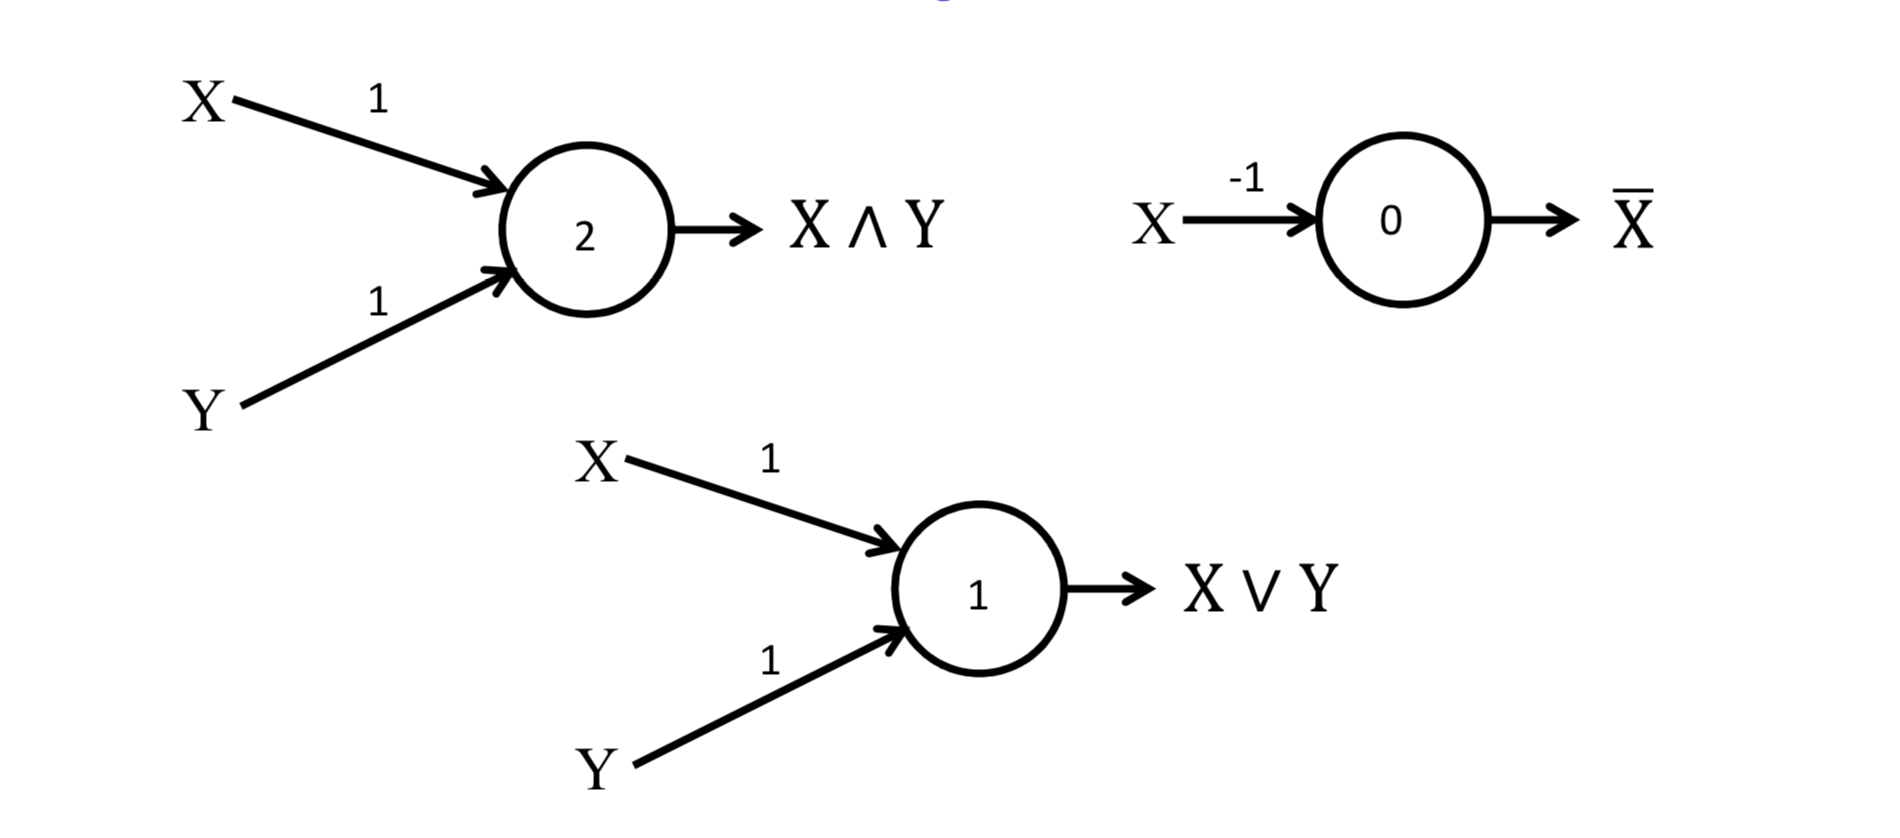
\includegraphics[scale=0.2]{1.png}
		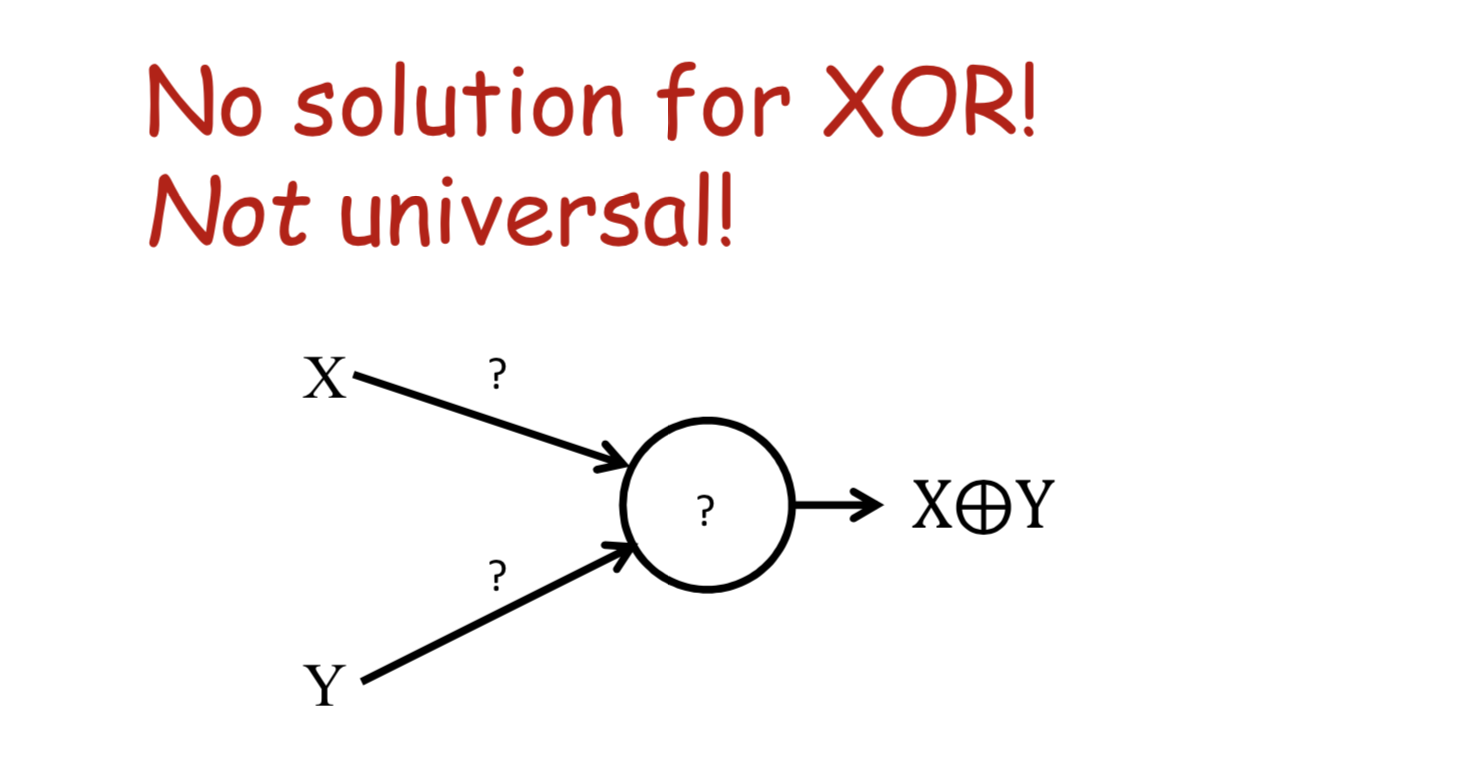
\includegraphics[scale=0.2]{2.png}
		
	\end{figure}
	
	
	\begin{itemize}
		\item Combine multiple perceptrons to represent XOR operations only when dealing with inputs and outputs (left figure)
	\end{itemize}


		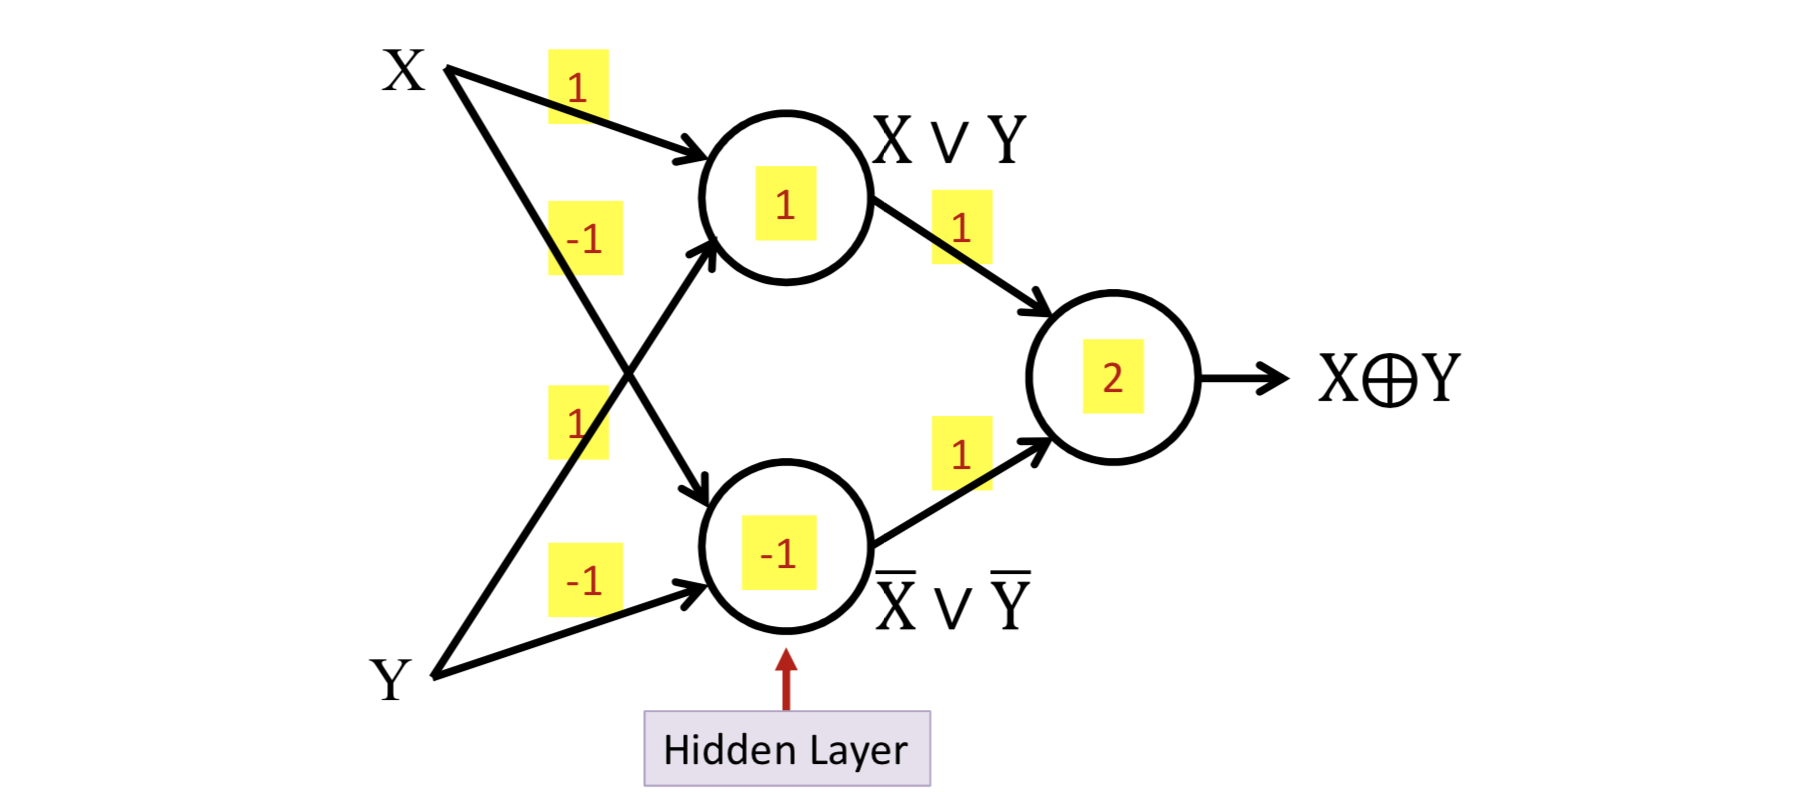
\includegraphics[scale=0.2]{3.png}
		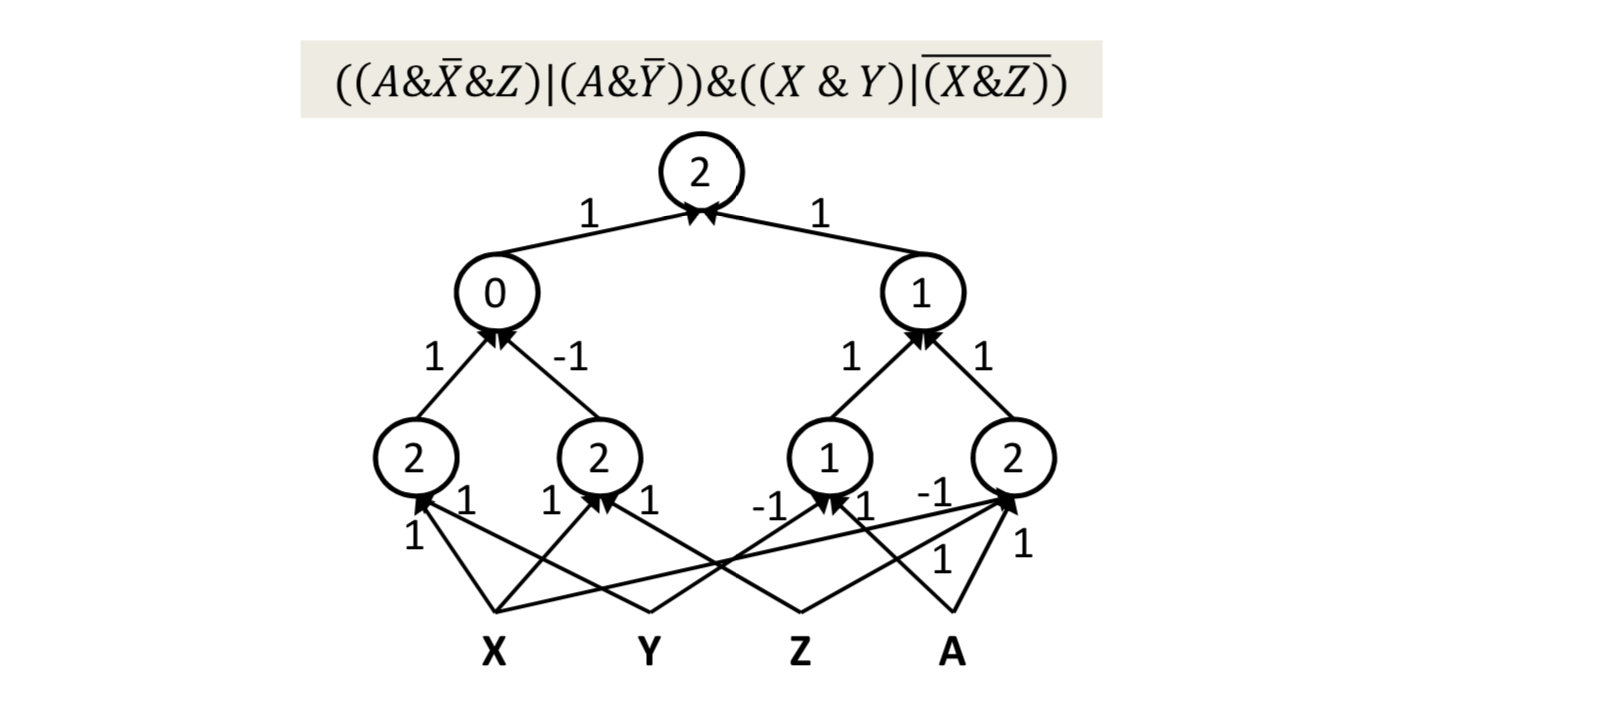
\includegraphics[scale=0.2]{4.png}

		
		
		\begin{itemize}
			\item Therefore, the perceptron has the ability to construct arbitrary functions of Boolean operations (right figure)
		\end{itemize}
		
		
		
	\textbf{2. Real input + discrete output: linear classifier}
	
		
		
		\begin{itemize}
			\item When the input and output are real, the perceptron is activated if the weighted sum exceeds the threshold. Essentially, the perceptual machine of real input will form a linear classifier.
		\end{itemize}
	
	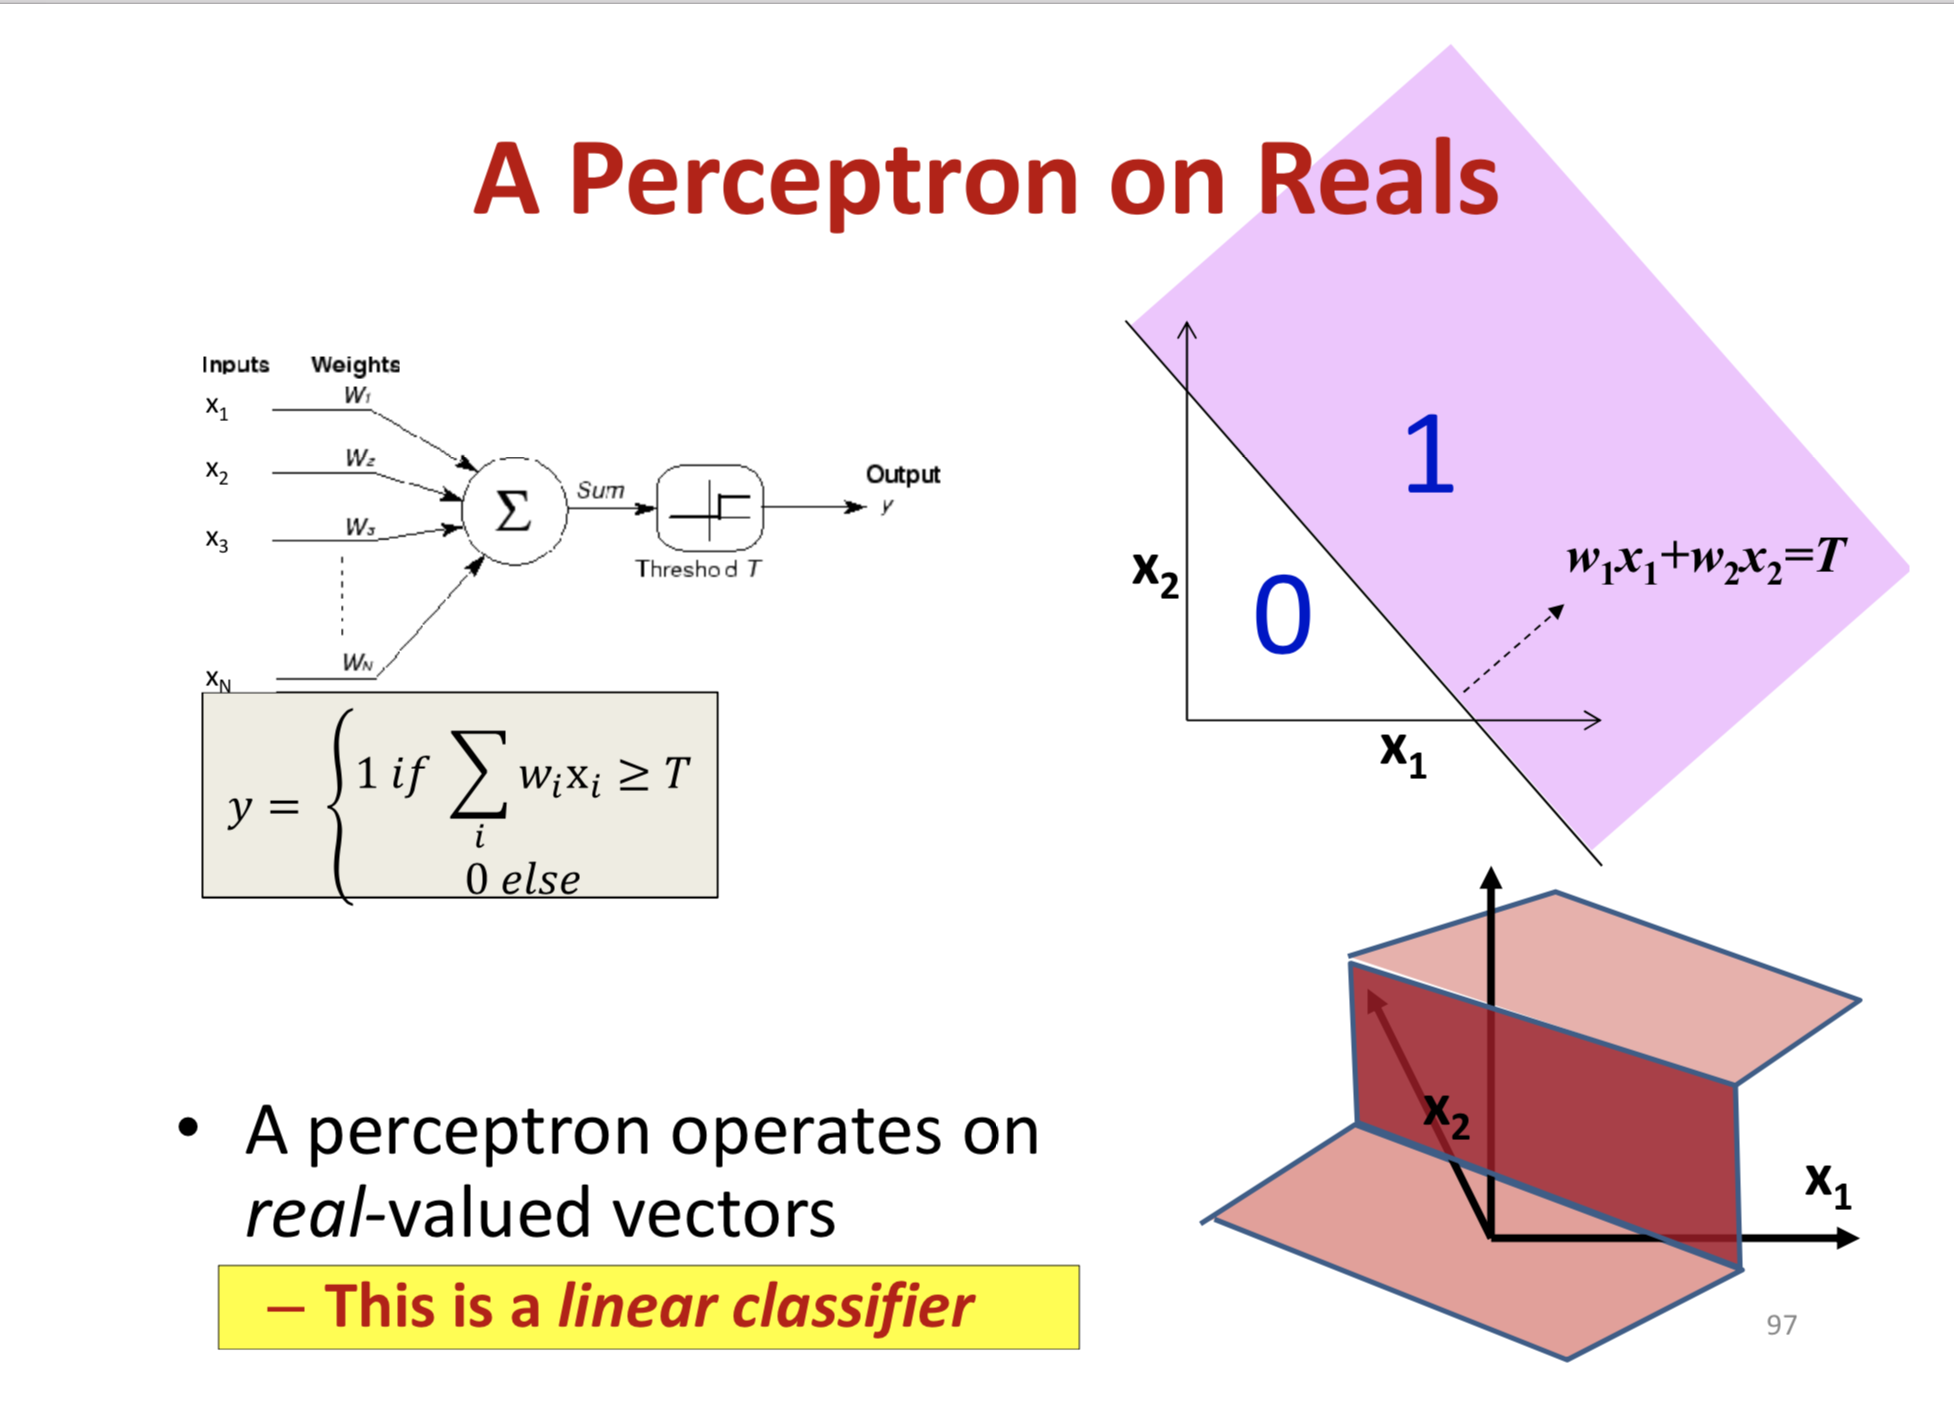
\includegraphics[scale=0.2]{5.png}
	
	
	\begin{itemize}
		\item It's easy to find 3 classifiers to fit Boolean operations (and/or/not), but XOR is impossible
	\end{itemize}

	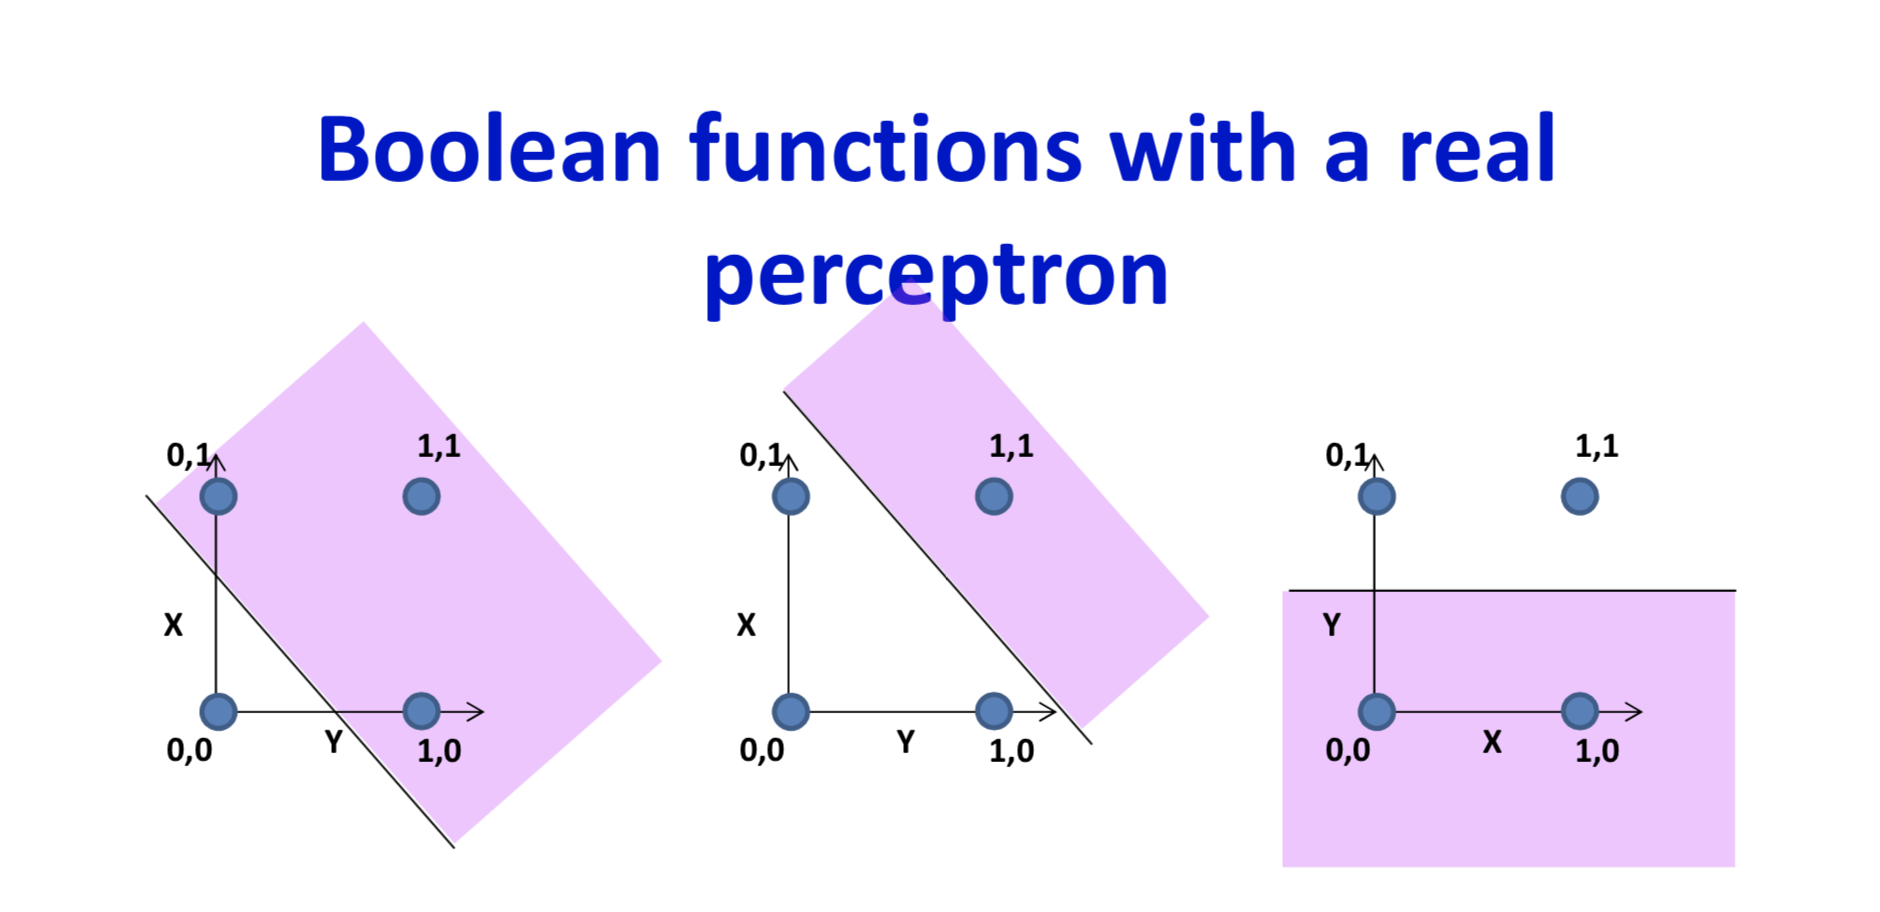
\includegraphics[scale=0.2]{6.png}
	
	\begin{itemize}
		\item Therefore, when any number of linear classifiers are properly combined, any decision surface can be represented
	\end{itemize}
	
	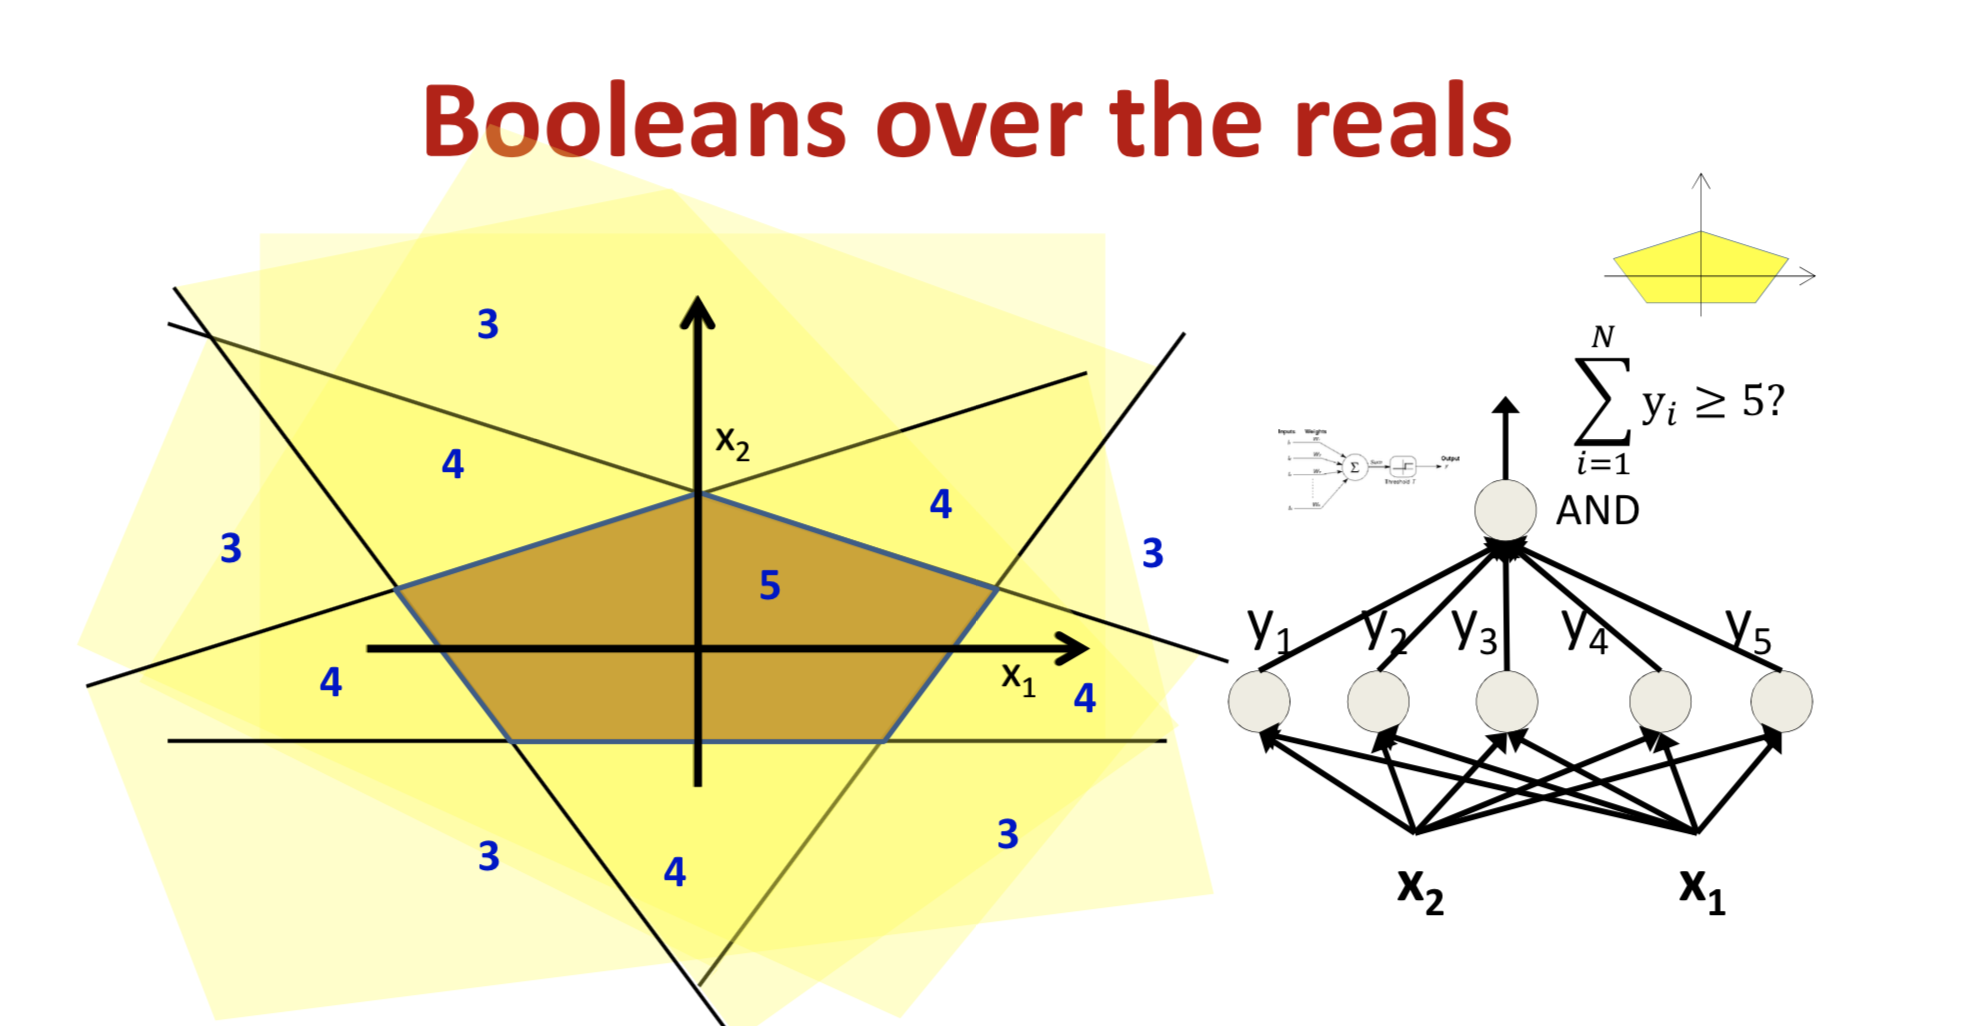
\includegraphics[scale=0.2]{7.png}
	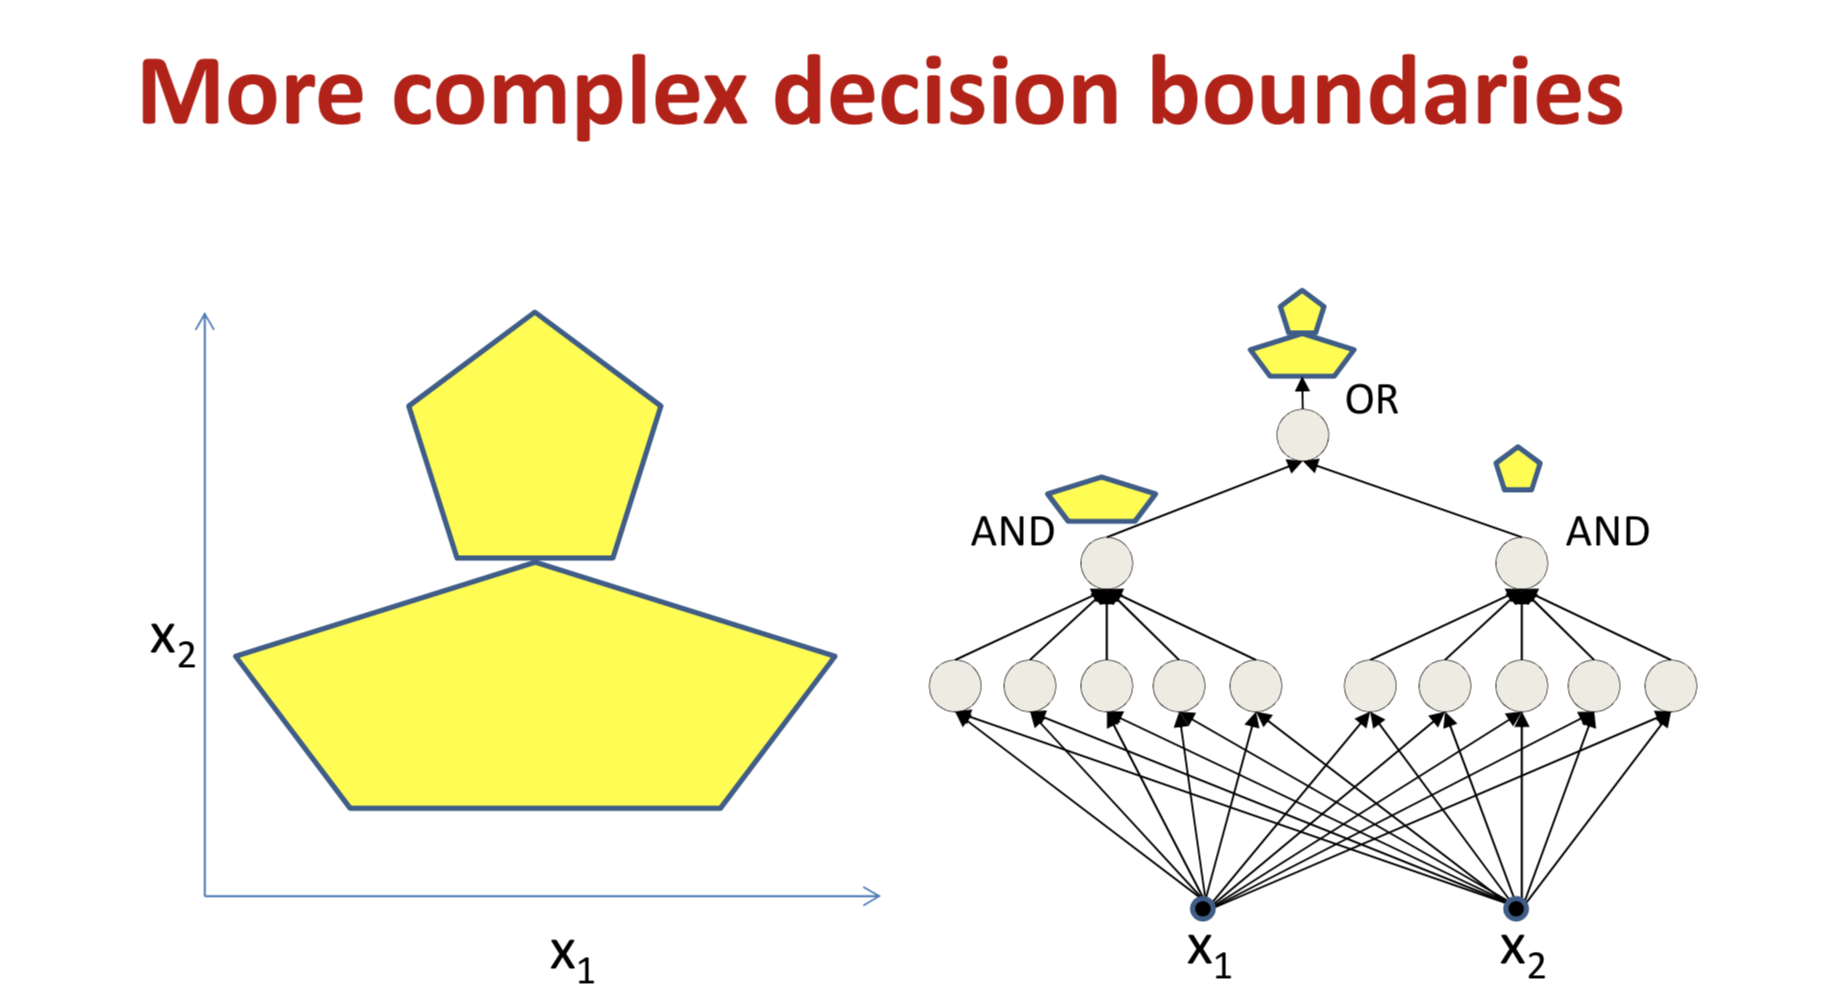
\includegraphics[scale=0.2]{8.png}
	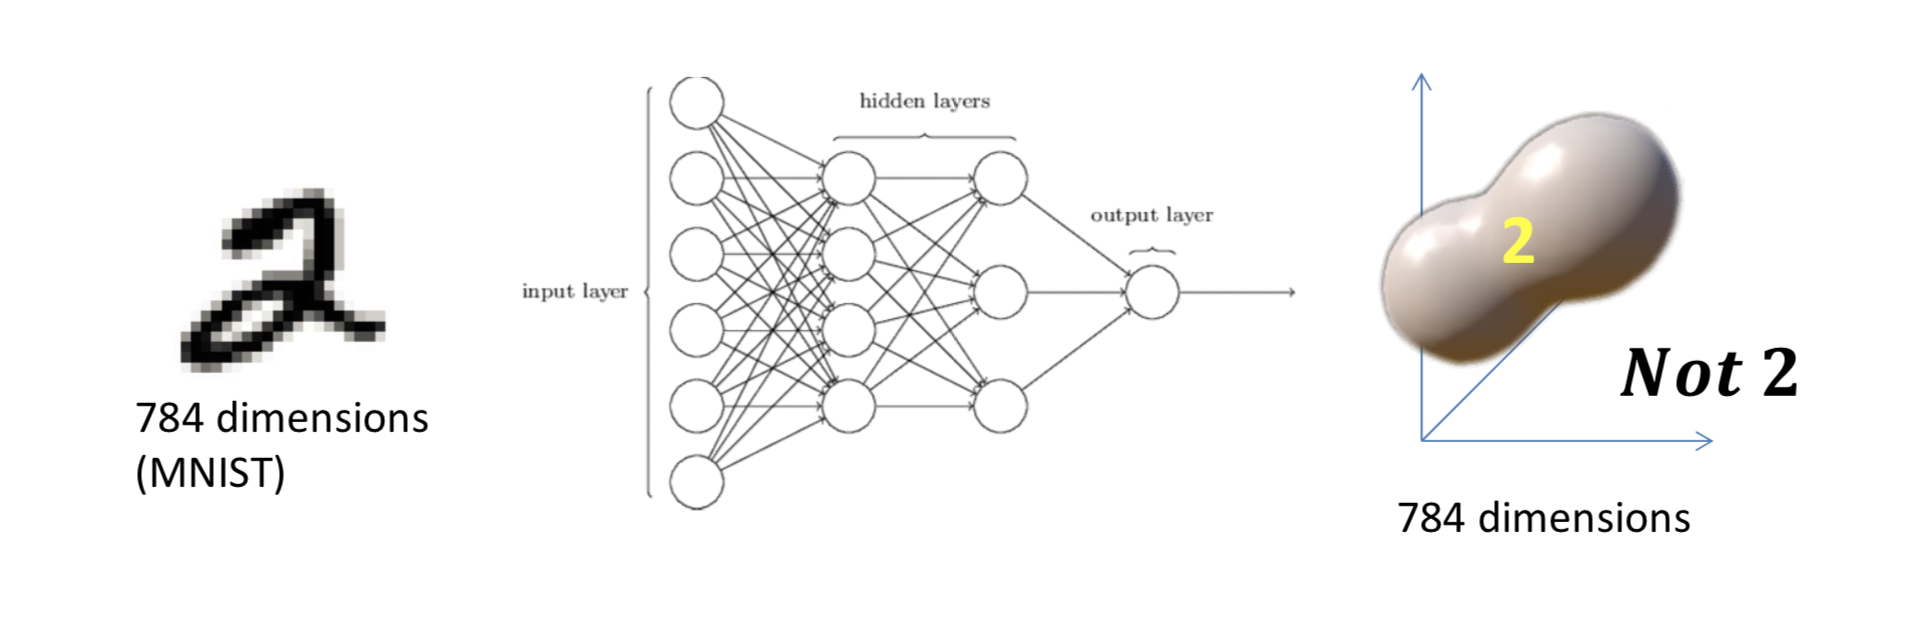
\includegraphics[scale=0.2]{9.png}
	
	
	\textbf{3. Real input + real output: regression problem}
	
	
		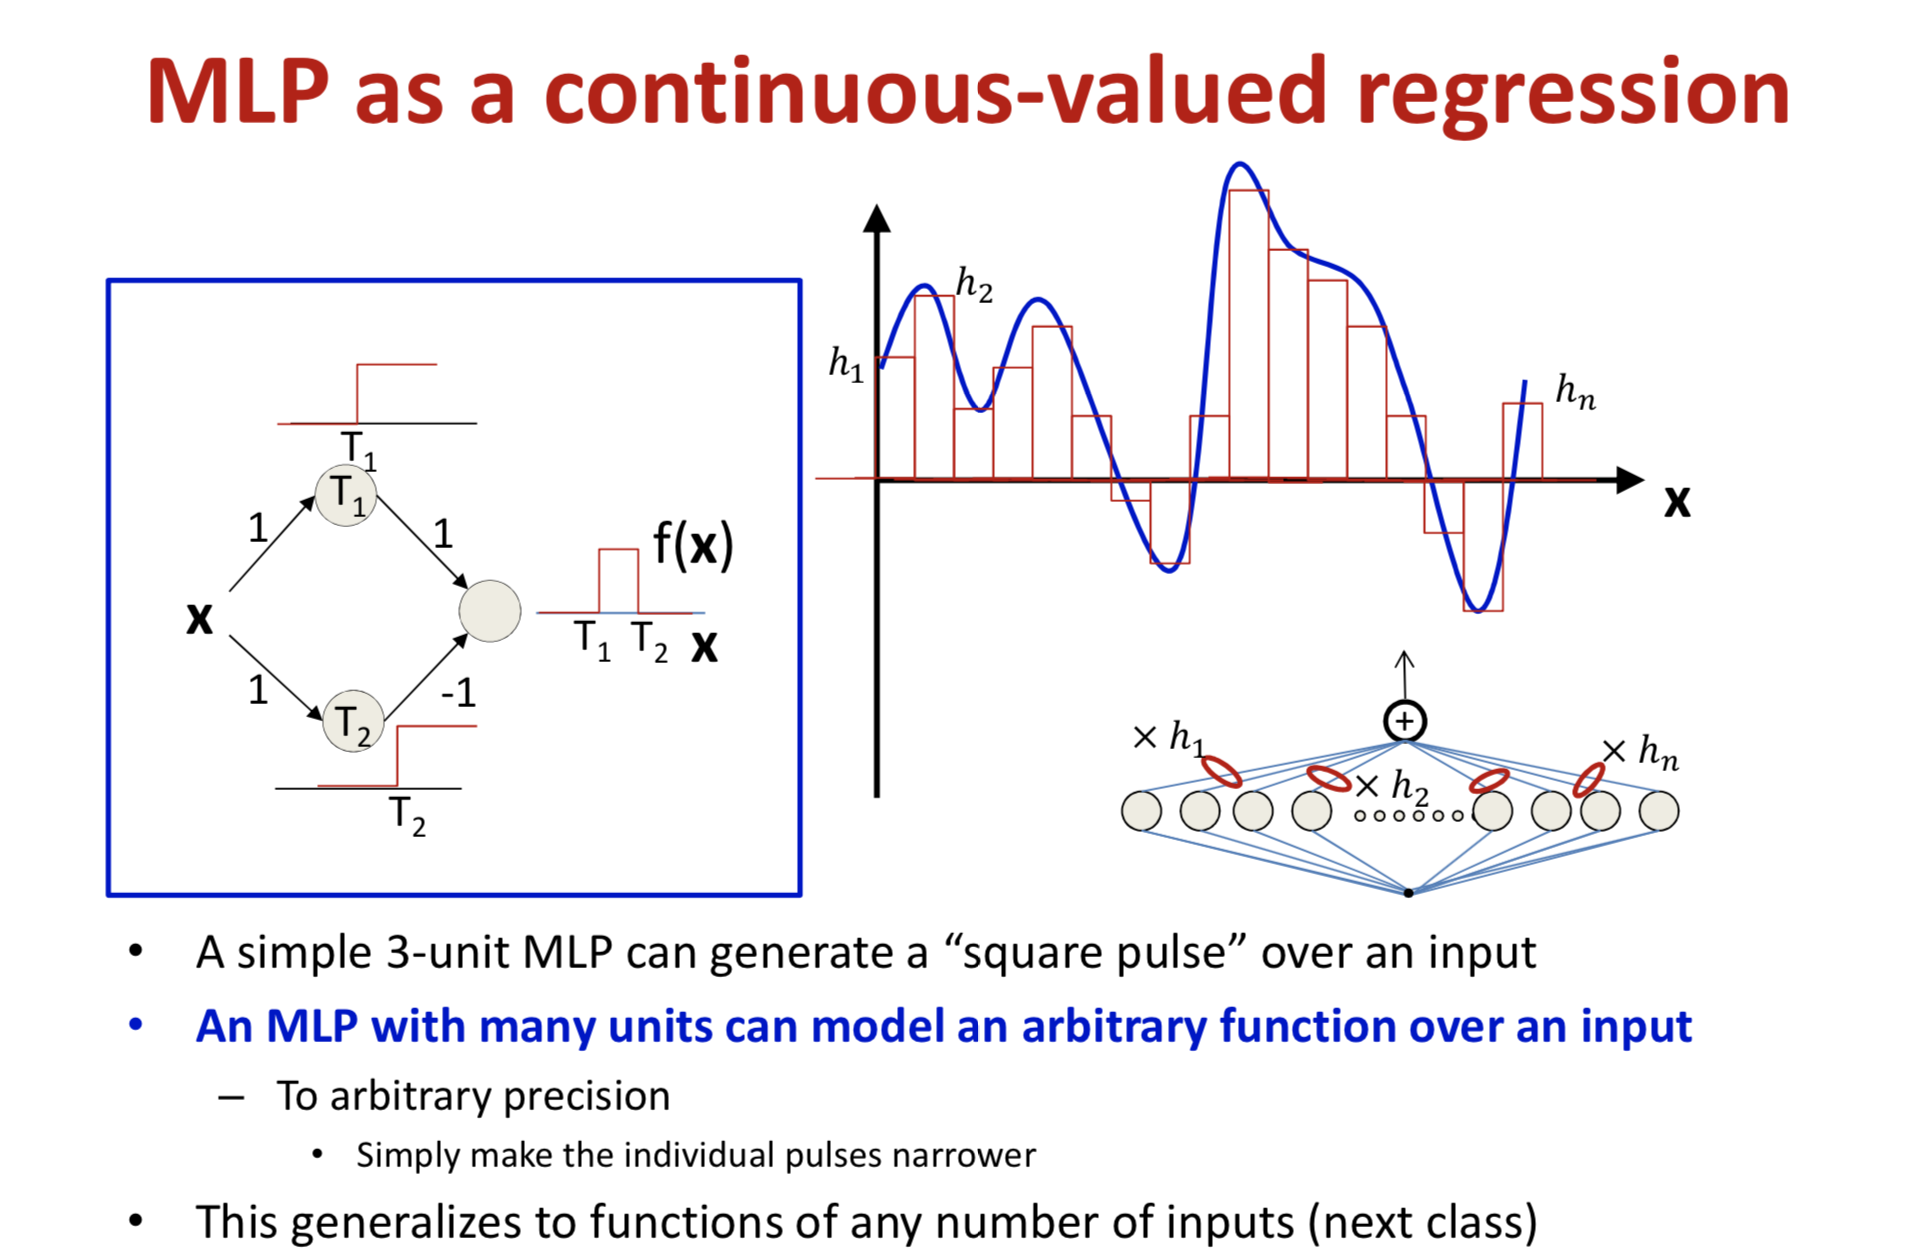
\includegraphics[scale=0.2]{10.png}
		
	
	\textbf{4. Intuitive reasons for modeling capabilities: the relationship between input $x$ and weight $w$}
		
		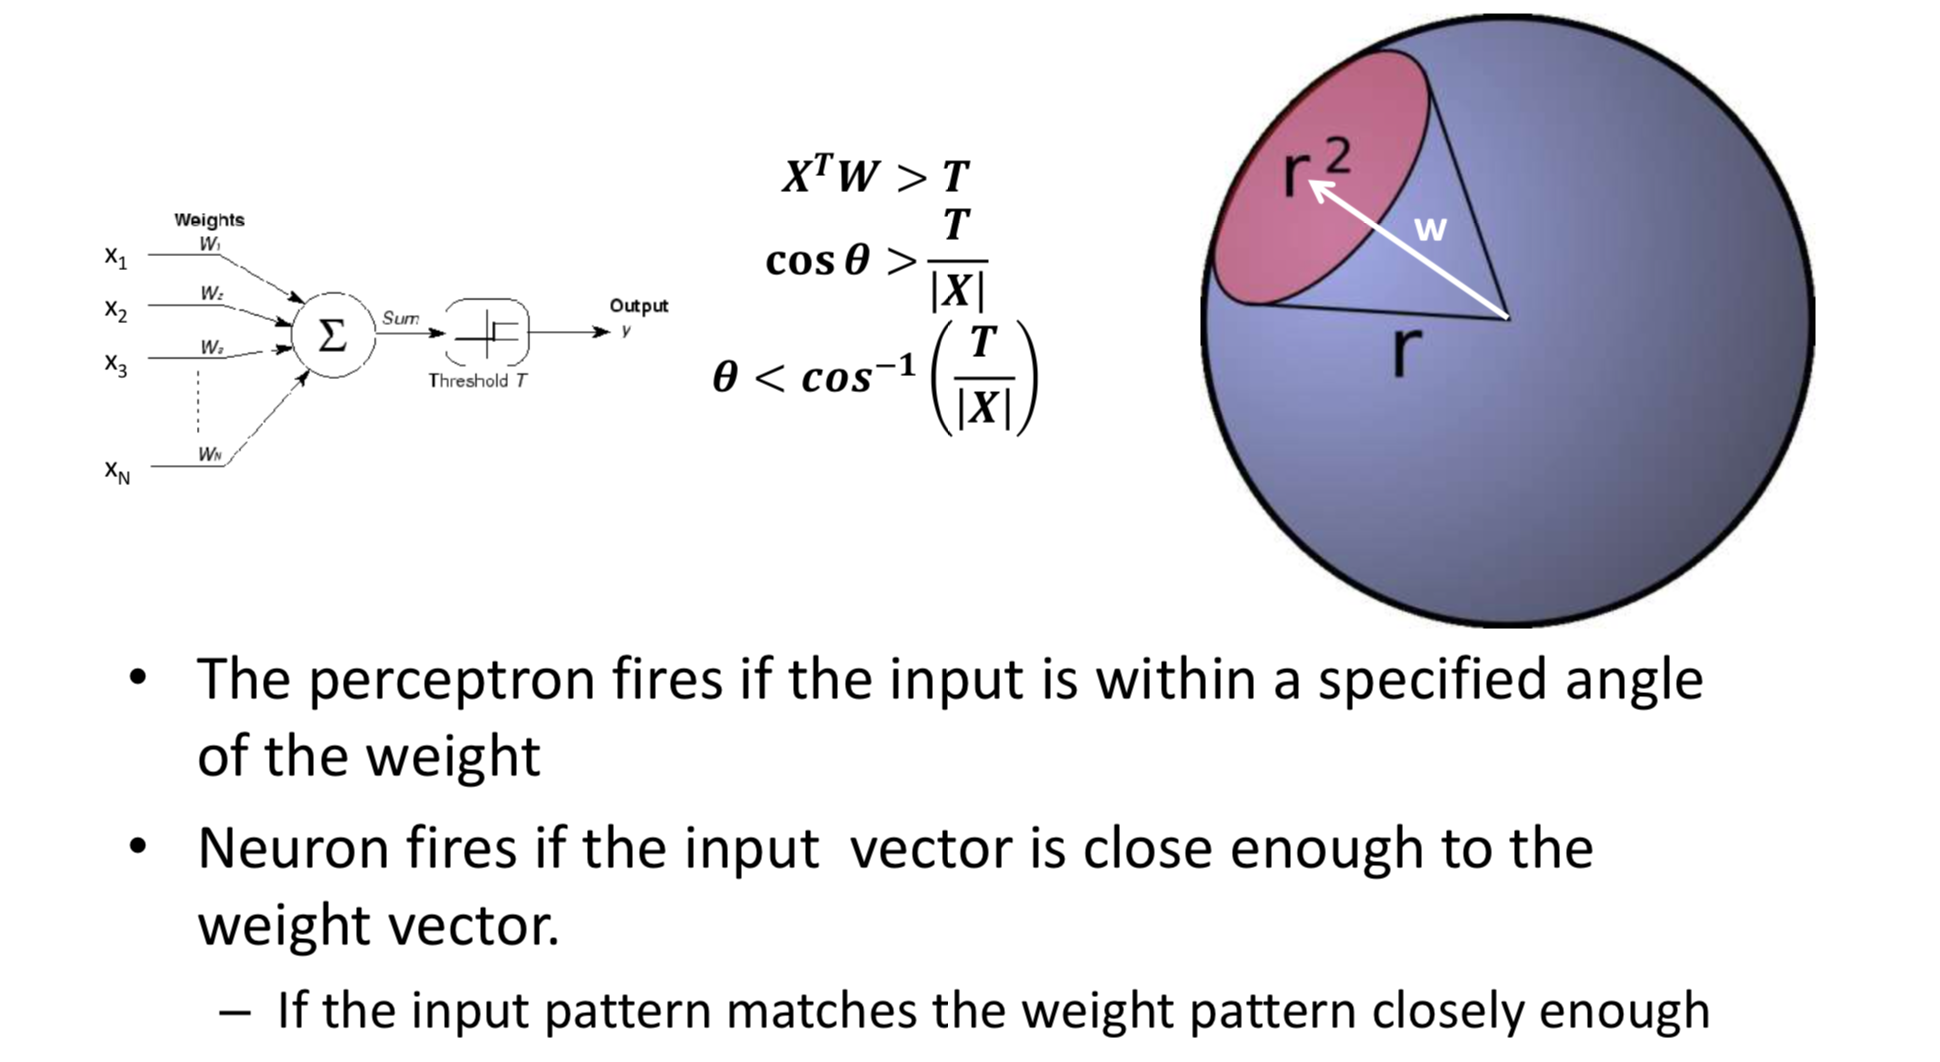
\includegraphics[scale=0.2]{11.png}
		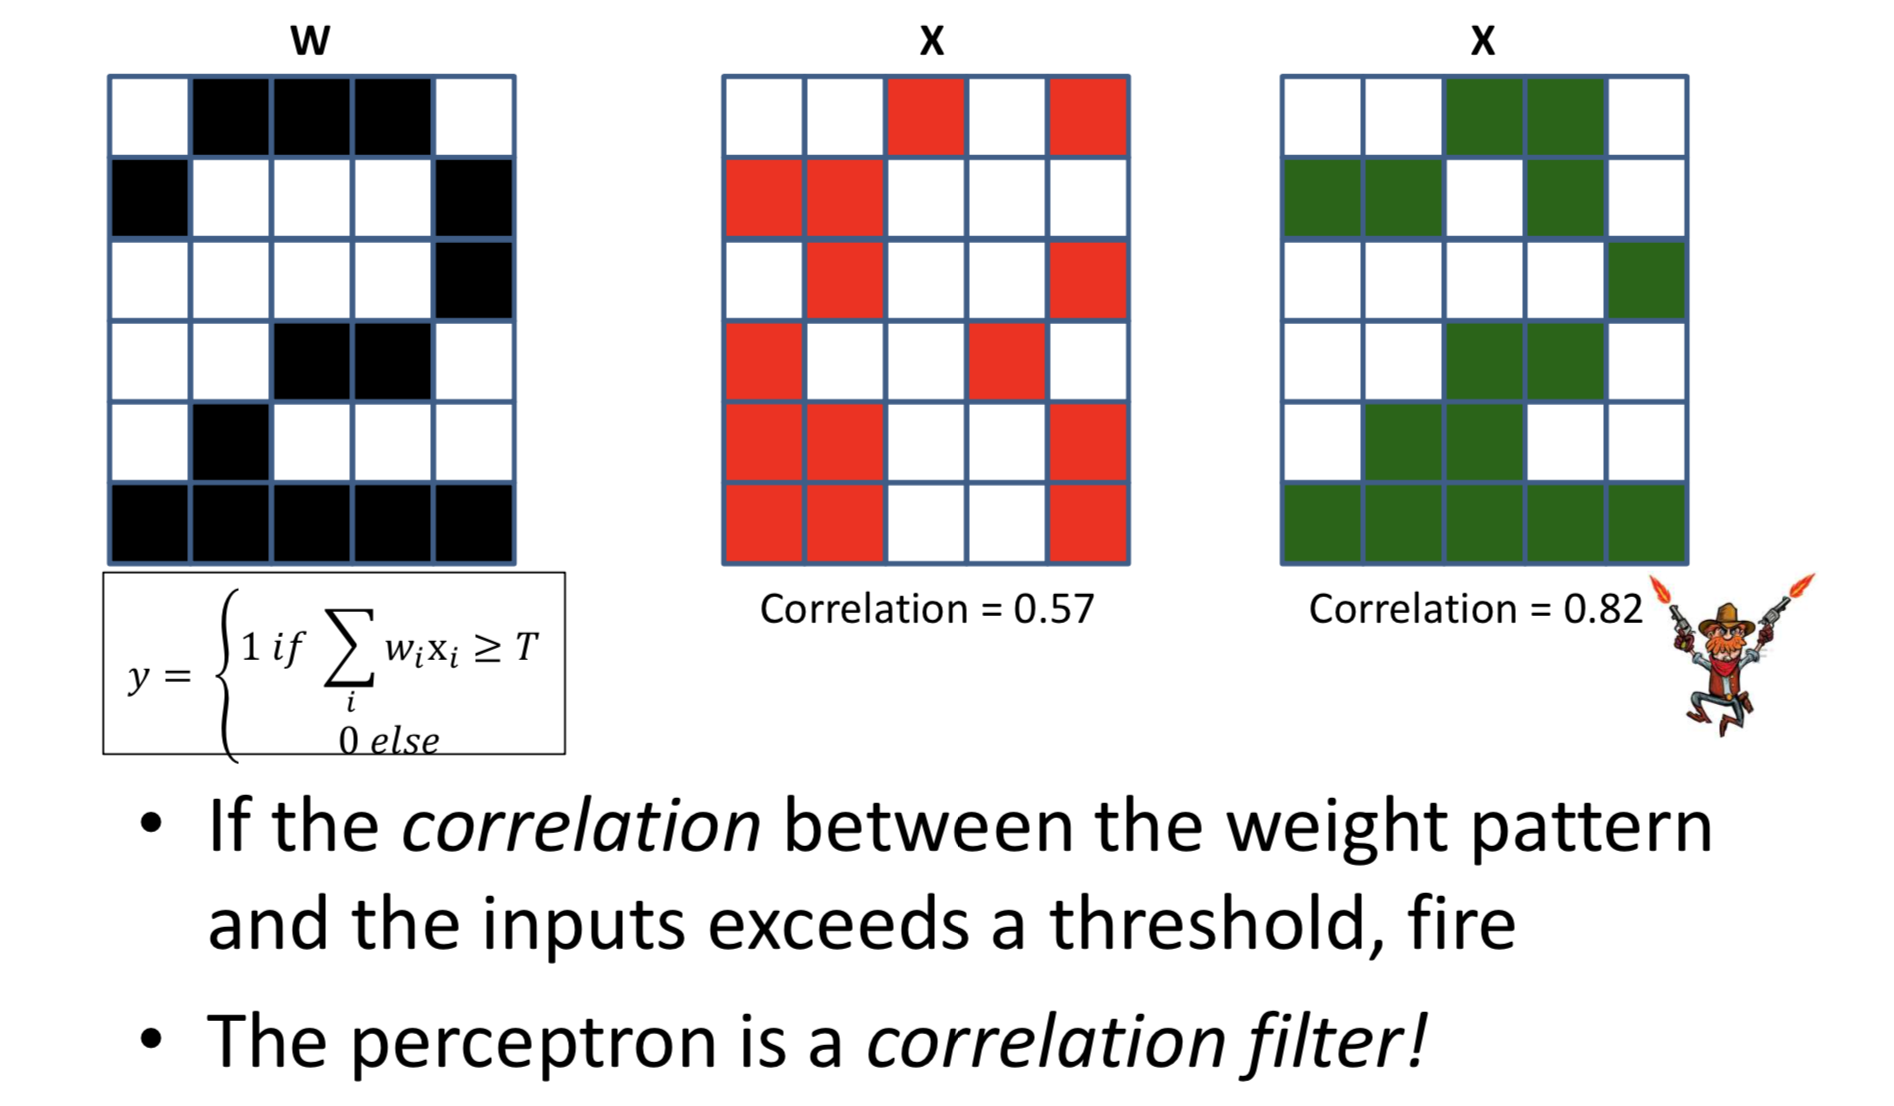
\includegraphics[scale=0.2]{12.png}
		
		In summary, the weight of the high-level perceptron reduces the input information of the lower layer as much as possible, and continuously retains and reorganizes the identified multiple features, thereby realizing the ability of pattern recognition.
		
		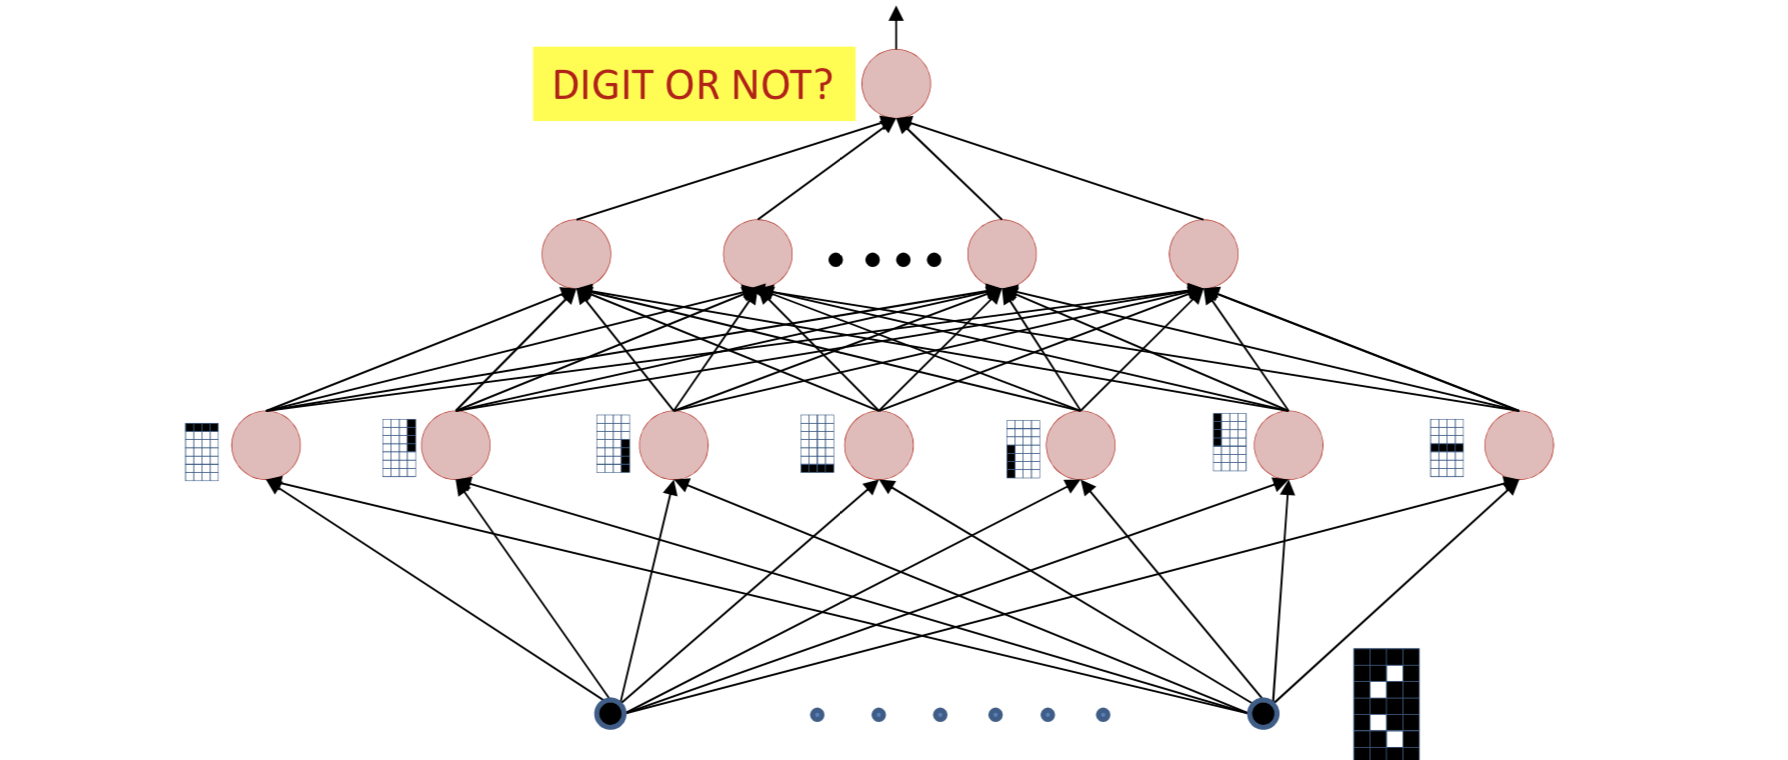
\includegraphics[scale=0.2]{13.png} \\ \\ \\ \\
		
		
		
{\LARGE 	\textbf{SUMMARY}}
	
	\begin{itemize}
		\item Neural network based AI has taken over most AI tasks
		\item Neural networks originally began as computational models
		of the brain \\
		- Or more generally, models of cognition
		\item The earliest model of cognition was associationism
		\item The more recent model of the brain is connectionist \\
		– Neurons connect to neurons \\
		– The workings of the brain are encoded in these connections 
		\item Current neural network models are connectionist machines
		– The comprise networks of neural units
		\item McCullough and Pitt model: Neurons as Boolean threshold units \\
		– Models the brain as performing propositional logic \\
		– But no learning rule
		\item Hebb’s learning rule: Neurons that fire together wire together \\
		– Unstable
		\item Rosenblatt’s perceptron : A variant of the McCulloch and Pitt neuron with a provably convergent learning rule \\
		– But individual perceptrons are limited in their capacity (Minsky and Papert) 
		\item Multi-layer perceptrons can model arbitrarily complex Boolean functions
		\item MLPs are classification engines \\
		– They can identify classes in the data \\ 
		– Individual perceptrons are feature detectors \\
		– The network will fire if the combination of the detected basic features matches an "acceptable" pattern for a desired class of signal
		\item MLP can also model continuous valued functions
		\item Perceptronsarecorrelationfilters \\
		– They detect patterns in the input
		\item Interesting AI tasks are functions that can be modelled by the network
		
	\end{itemize}



		
	\subsection{MLP: Theoretical Proof}
	
	
	\textbf{\textit{Question: Why can a neural network be used as a universal approximator to fit any function? --- Theoretical Proof}}
	
	Lecture1 mainly introduces the neural network as an intuitive understanding of the universal approximator. Lecture2 turns to a more in-depth theoretical proof, which is still discussed from three aspects: Boolean operation, linear classifier and regression problem.
	
	
	\textbf{1. Boolean operation}
	
	Multi-layer perceptrons can construct Boolean operations in any form and combination. Then, how many layers and how many neurons are perceived by a common Boolean function? \\ \\
		
		\begin{itemize}
			\item Truth Table + DNF Formula: Exhaustive Method
		\end{itemize}
	
	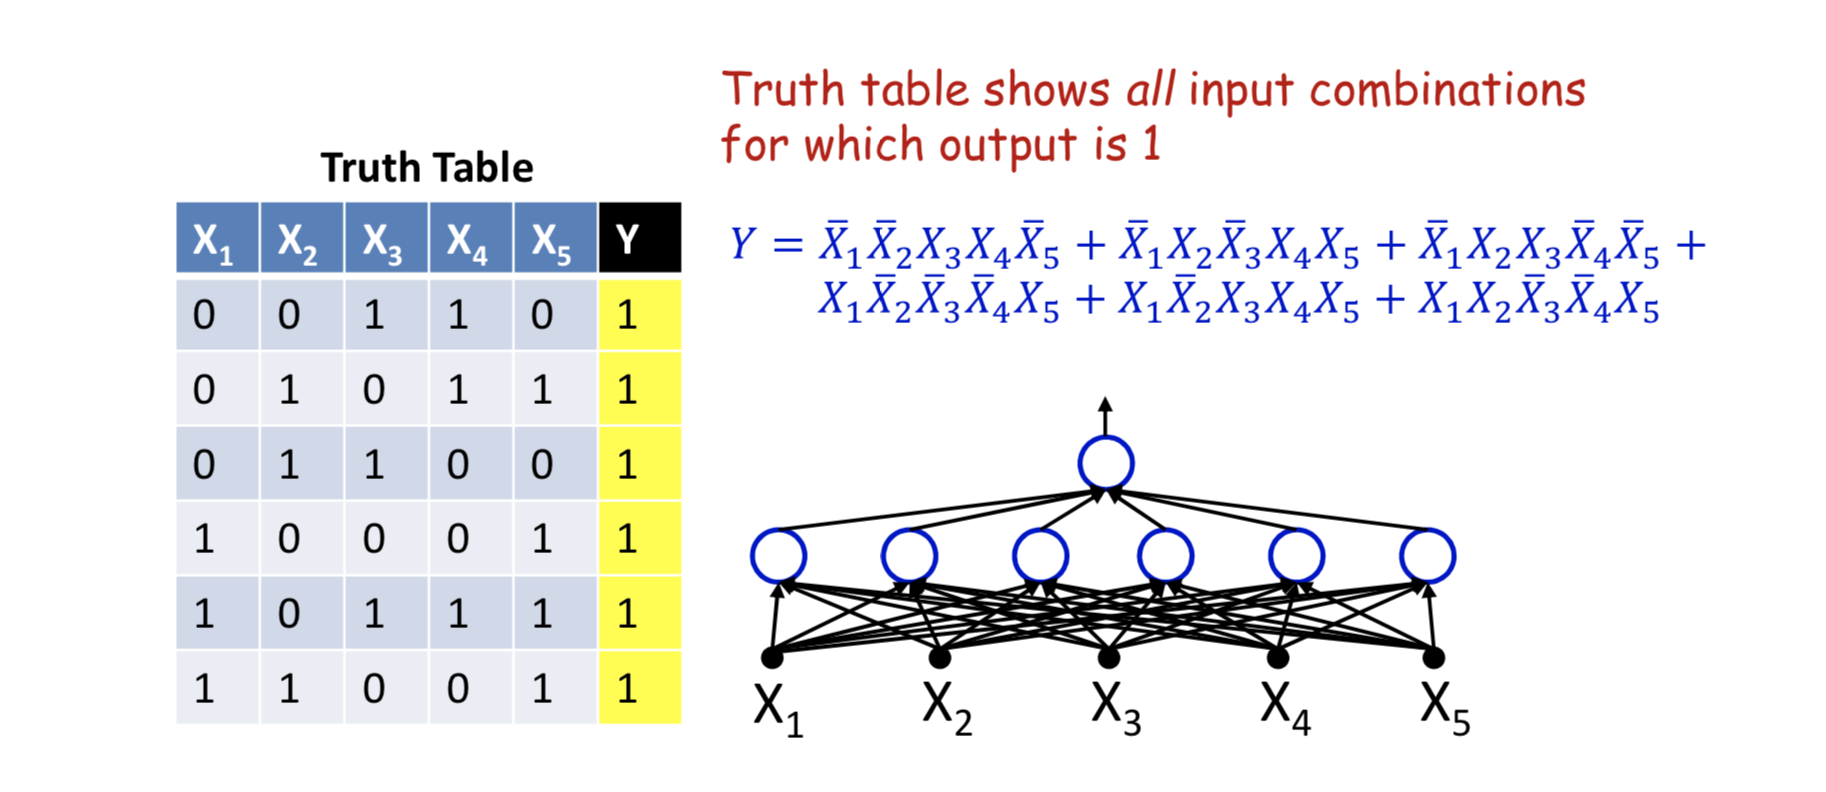
\includegraphics[scale=0.2]{14.png}
	
	Notes: Any Boolean operation can be exhausted by the truth table. Each row of the truth table corresponds to each item of the DNF formula. Each item of the DNF formula corresponds to each node of the network hidden layer.
	
	Conclusion 1.1: A one-hidden-layer MLP is a Universal Boolean Function
		
	
		\begin{itemize}
			\item Karnaugh map: simplification of truth table
		\end{itemize}
	
	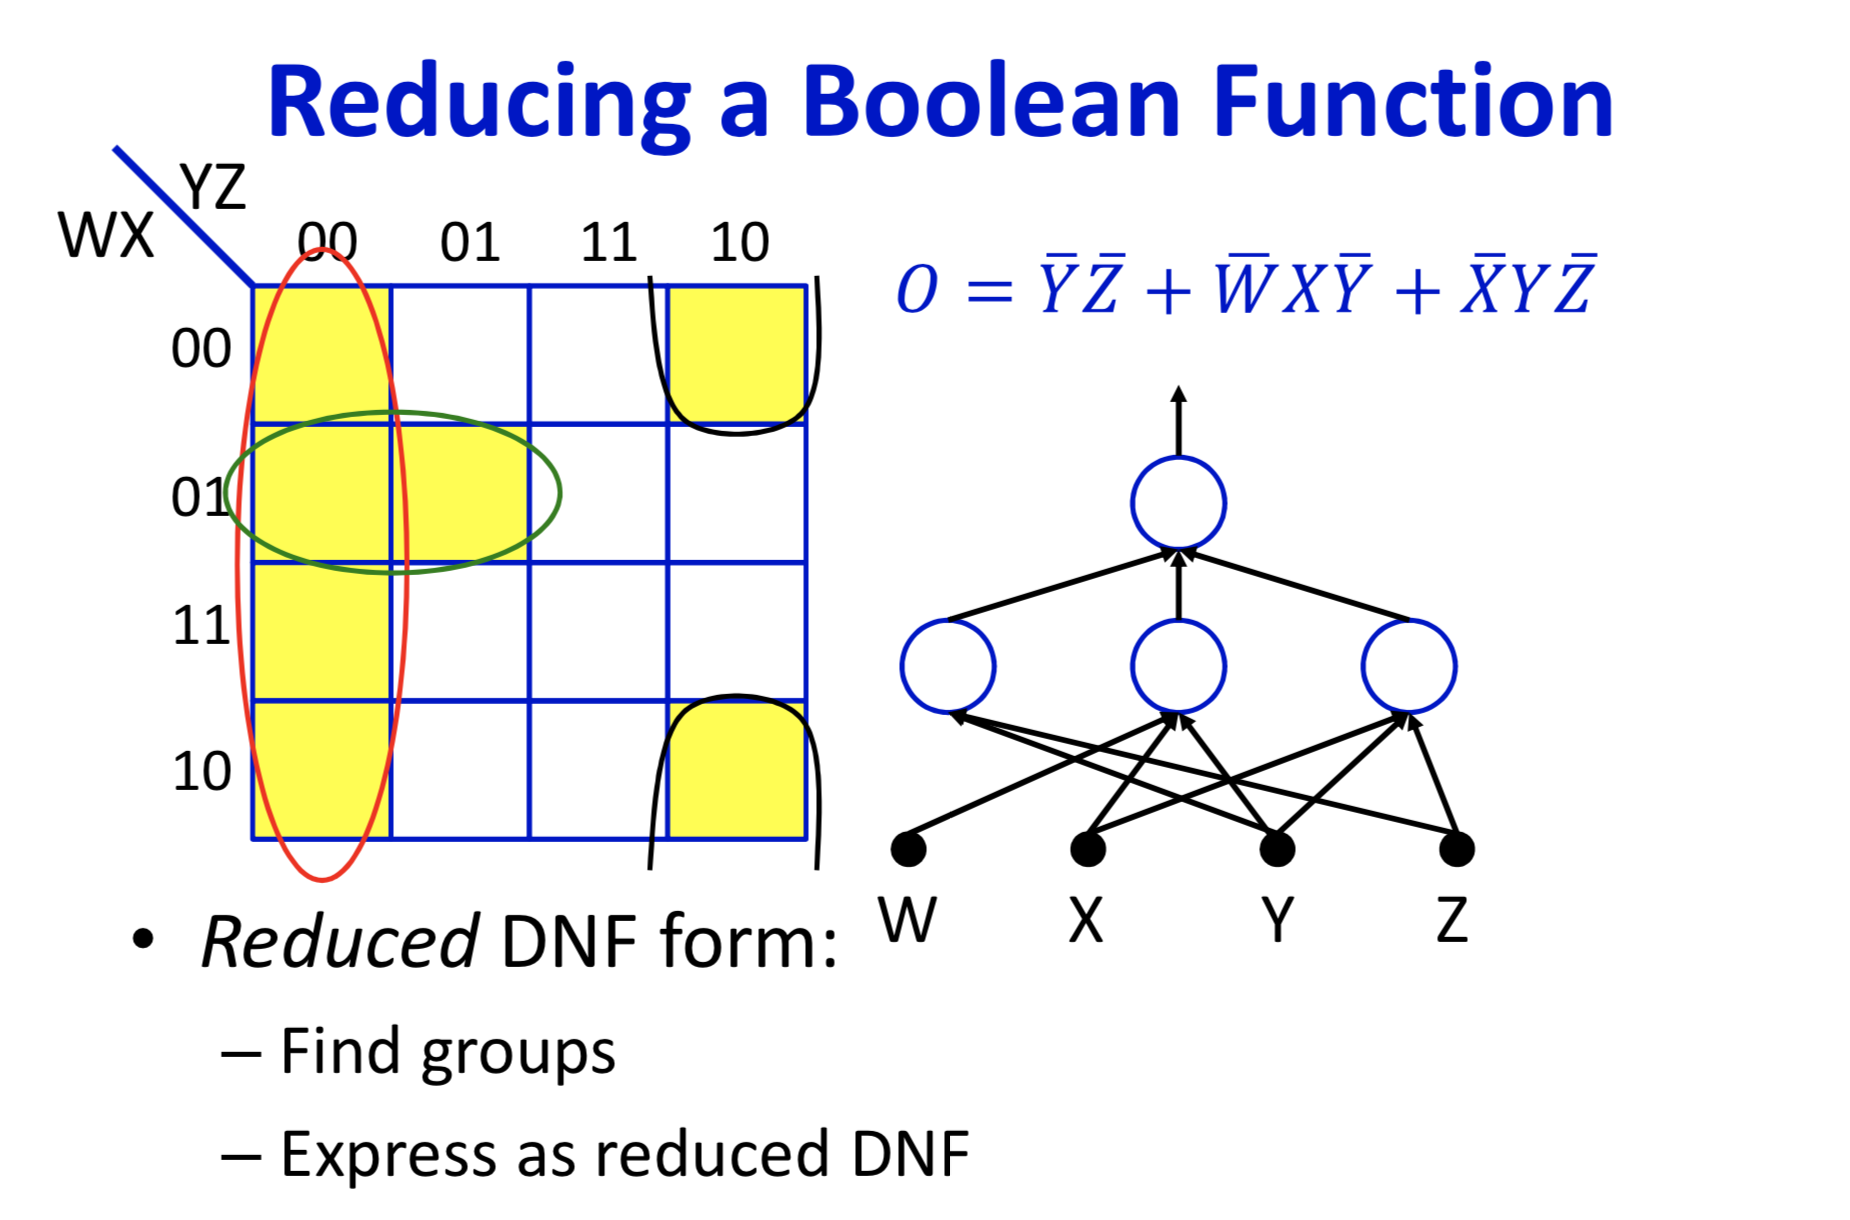
\includegraphics[scale=0.2]{15.png}
	
	Notes: A four-variable Karnaugh map with yellow for 1 and white for 0. Combine the maximum $2^n$ yellow 1 adjacent to the horizontal/vertical direction to simplify the truth table DNF formula, thus simplifying the number of hidden layers.
	
	\textbf{Worst case:} In the Karnaugh map, any squares with a true value of 1 cannot be merged, and the DNF formula cannot be simplified.
	
	
	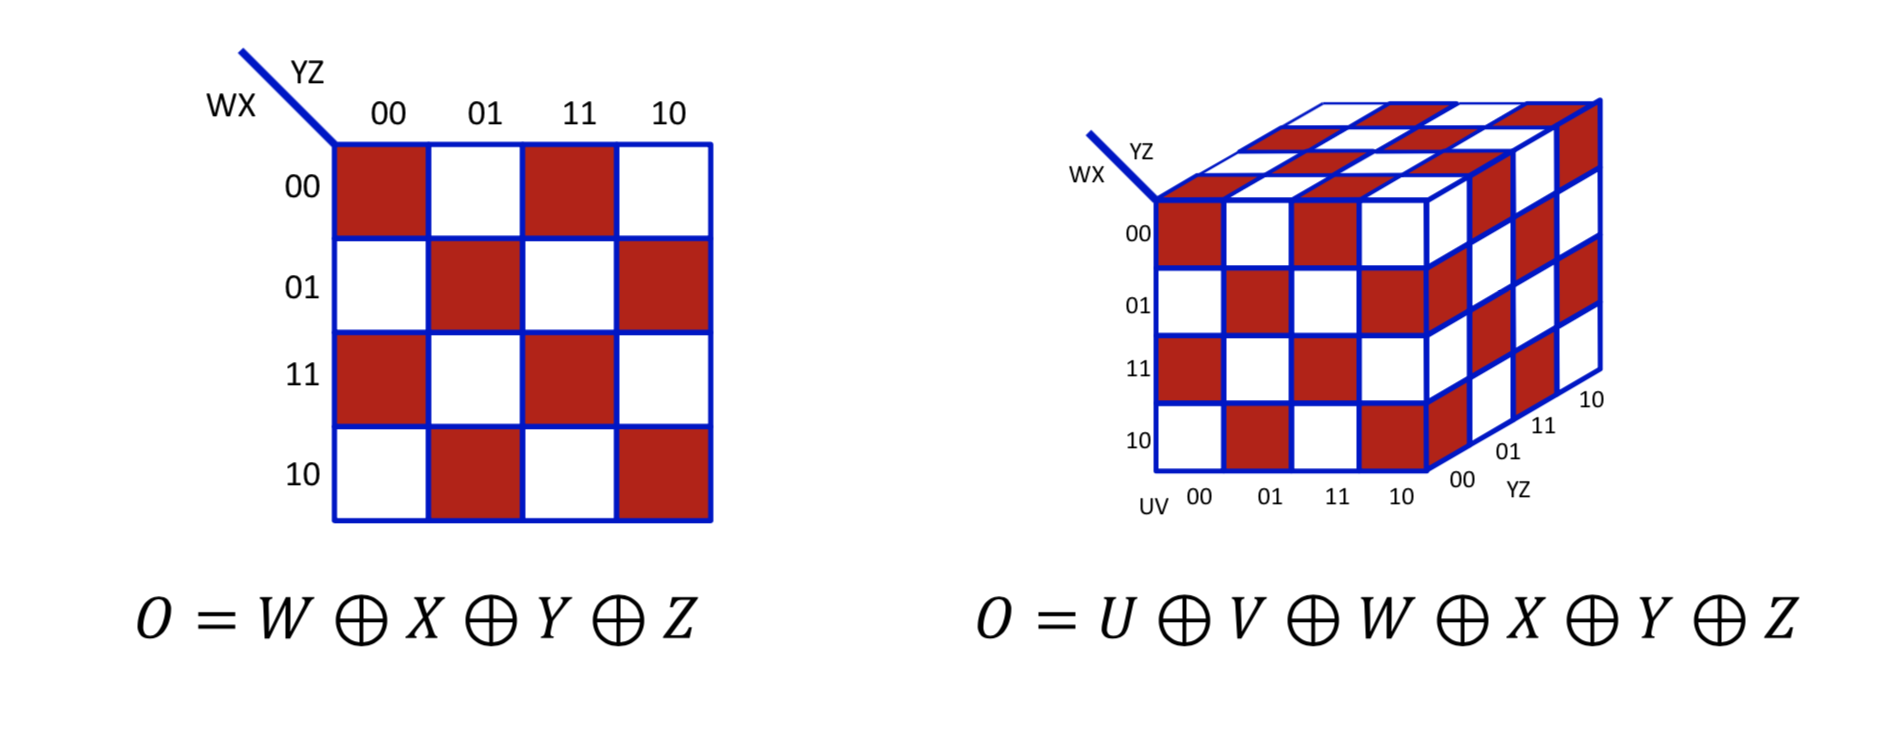
\includegraphics[scale=0.2]{16.png}
	
	Conclusion 1.2: Under the worst Karnaugh map, the maximum number of neurons in a layer of perceptron networks is $2^{N-1}$. That is, the number of white squares. The number of neurons is an exponential multiple of the number of variables. \\ \\ \\
	
	
	\begin{itemize}
		\item In the worst case, use the XOR method: increase the number of layers and reduce the number of neurons
	\end{itemize}
	
	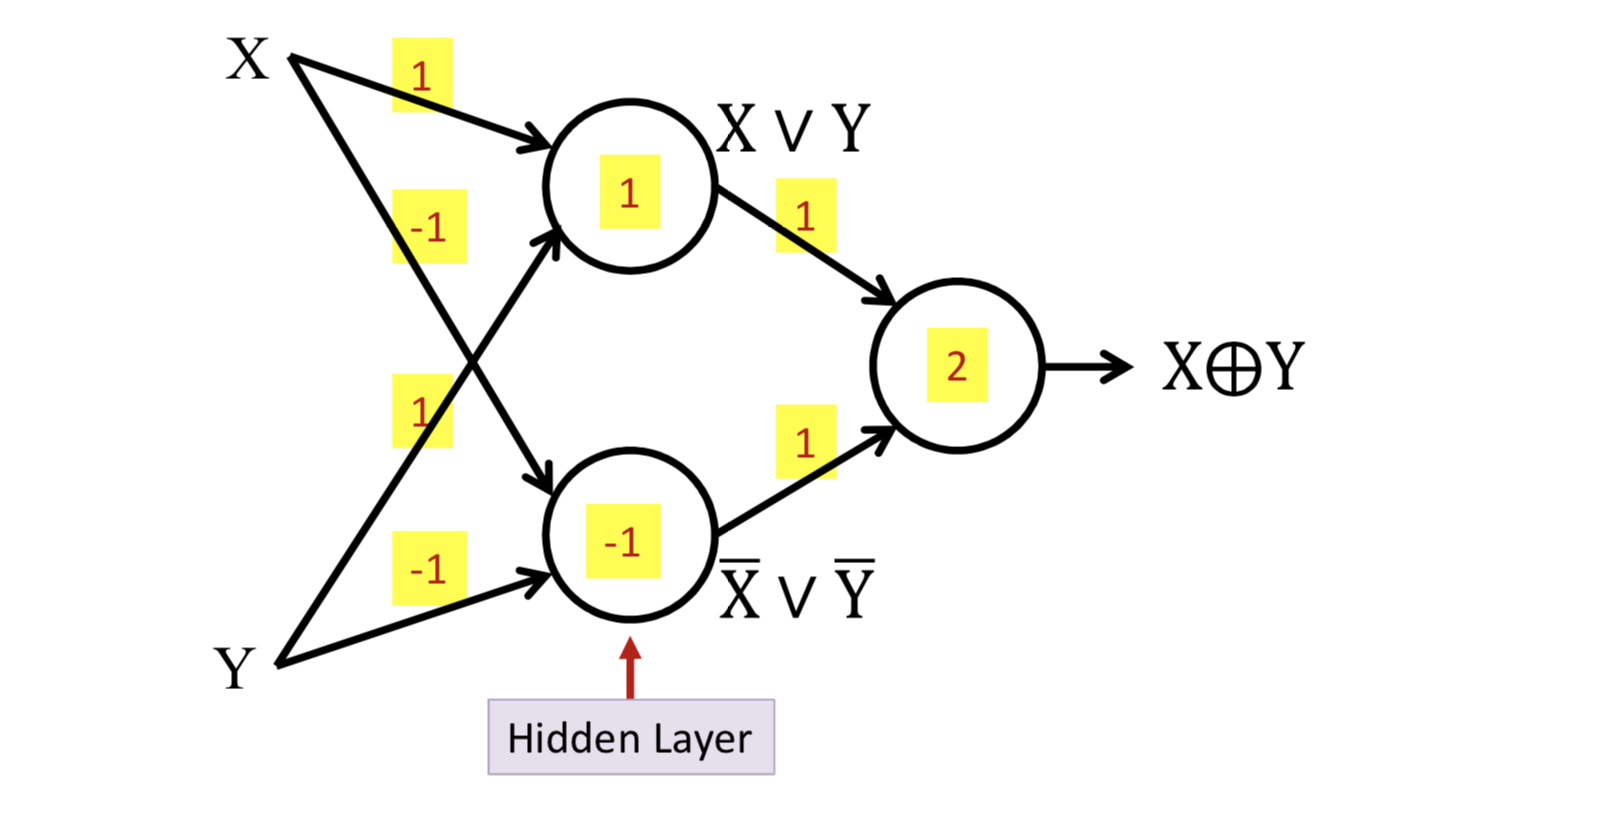
\includegraphics[scale=0.2]{17.png}
	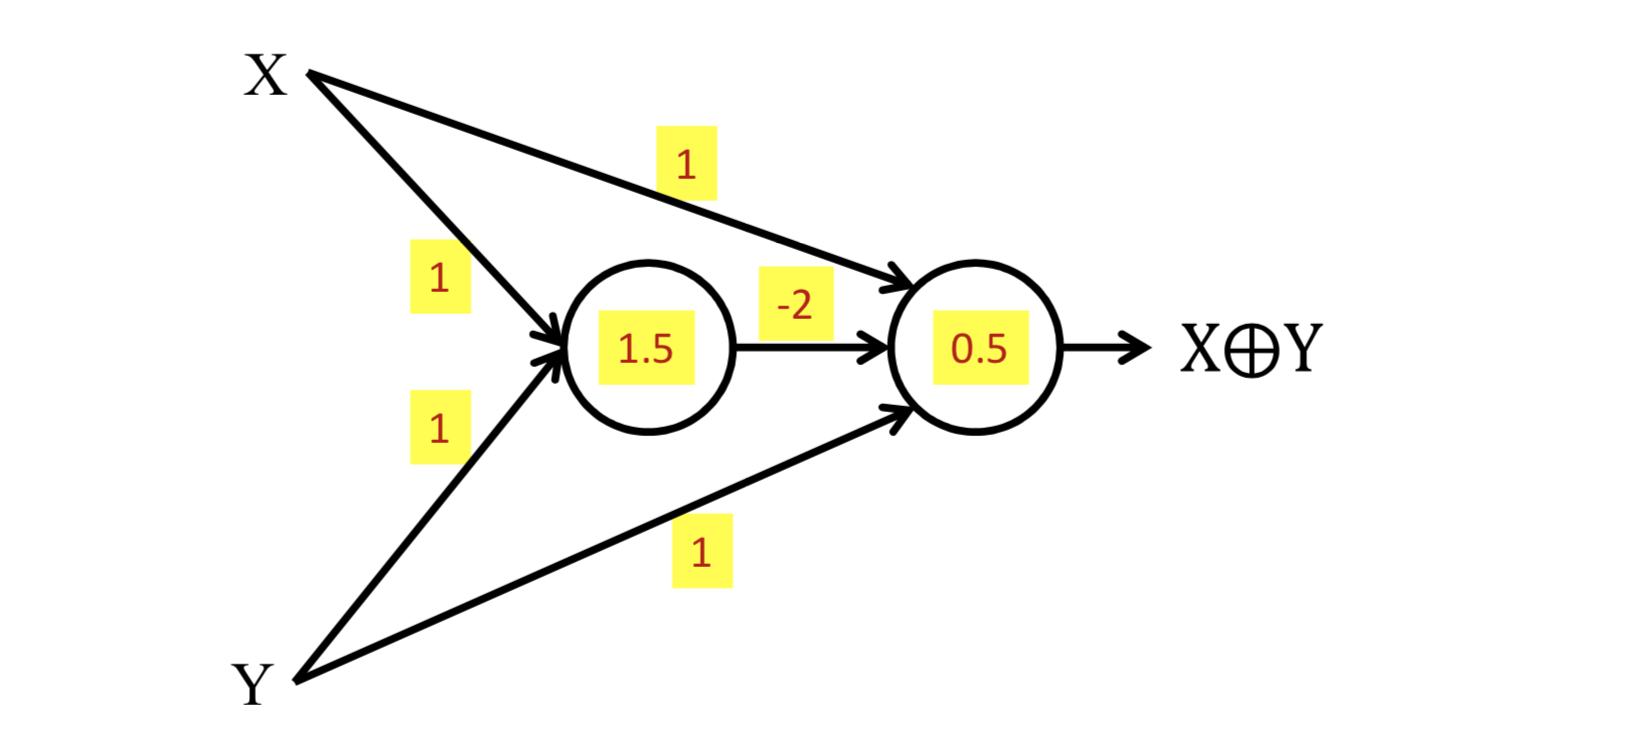
\includegraphics[scale=0.2]{18.png}
	
	Notes: Two representations of XOR.
	
	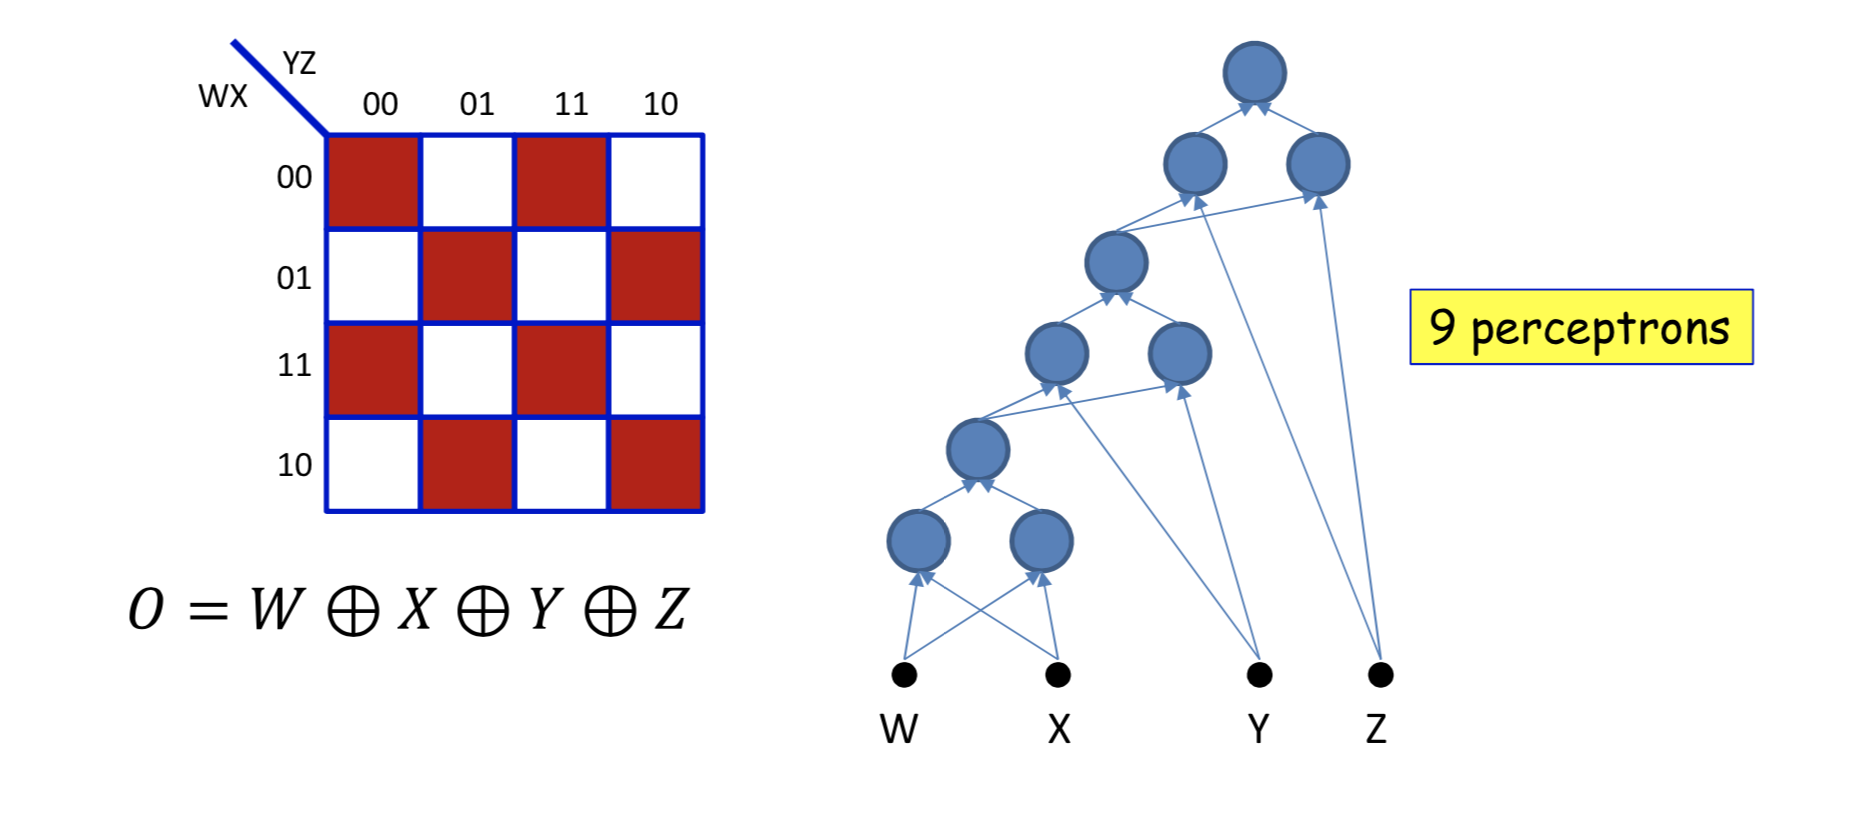
\includegraphics[scale=0.2]{19.png}
	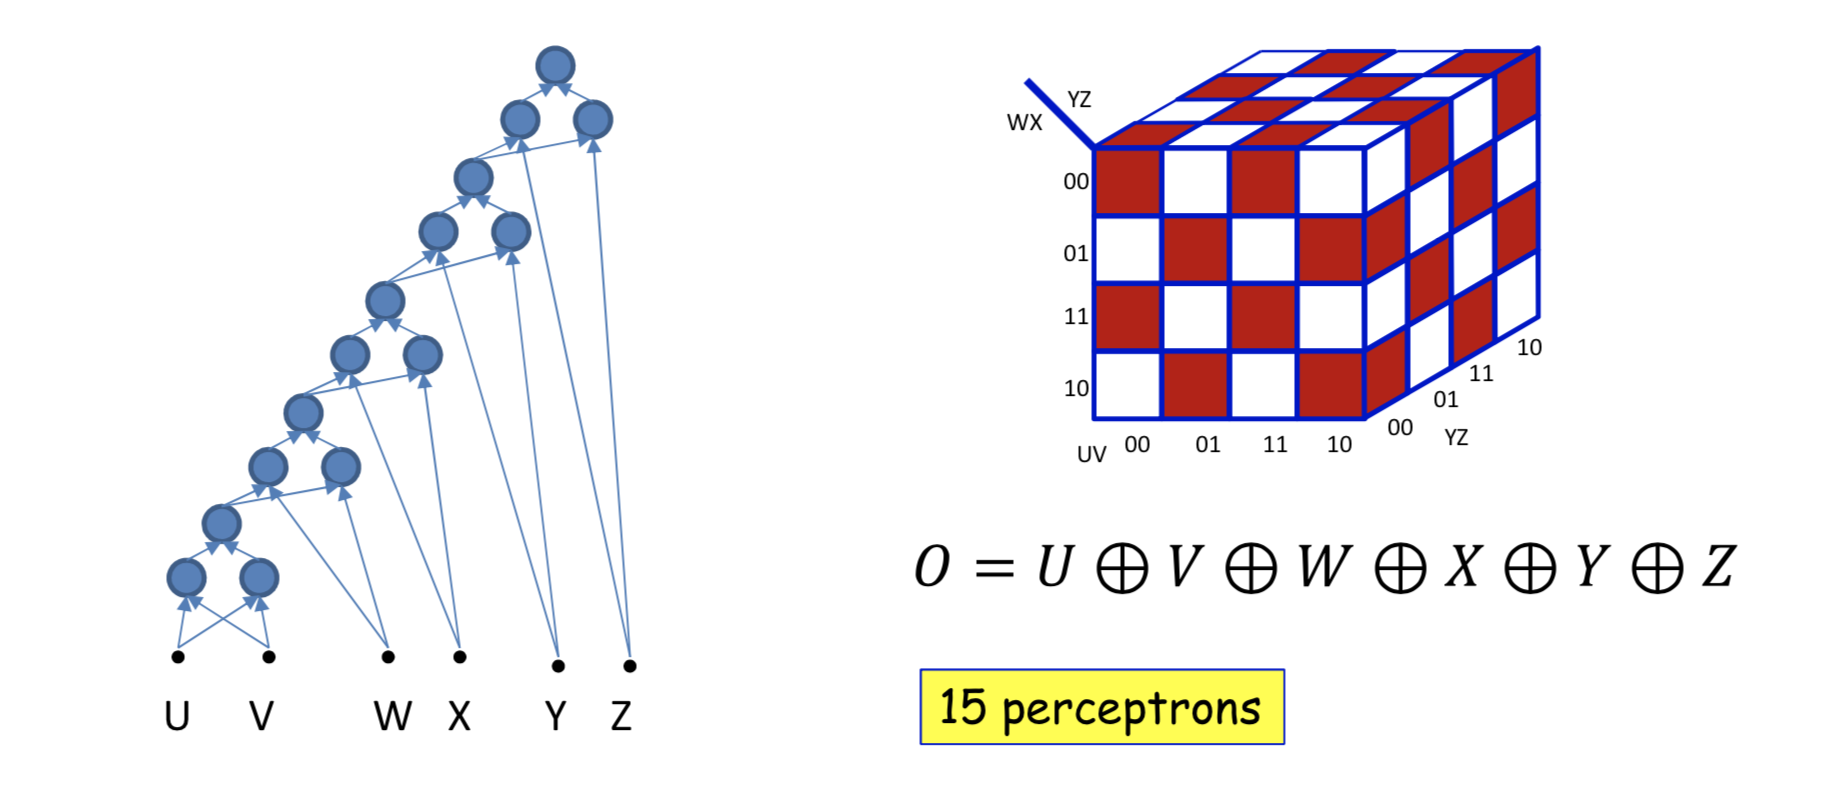
\includegraphics[scale=0.2]{20.png}
	
	Notes: In the worst case four-variable and six-variable Karnaugh maps, use the XOR method to increase the number of layers and reduce the number of neurons.
	
	Conclusion 1.3: Under the worst-case Karnaugh map, the maximum number of neurons in a multi-layer perceptron network is $3 (N-1)$ or $2 (N-1)$, and the number of network layers is $2 (N-1)$ using the XOR method. The number of neurons and the number of network layers are constant multiples of the number of variables.
	
	\begin{itemize}
		\item In the worst case, the law of the XOR method: reducing the number of layers
	\end{itemize}
	
	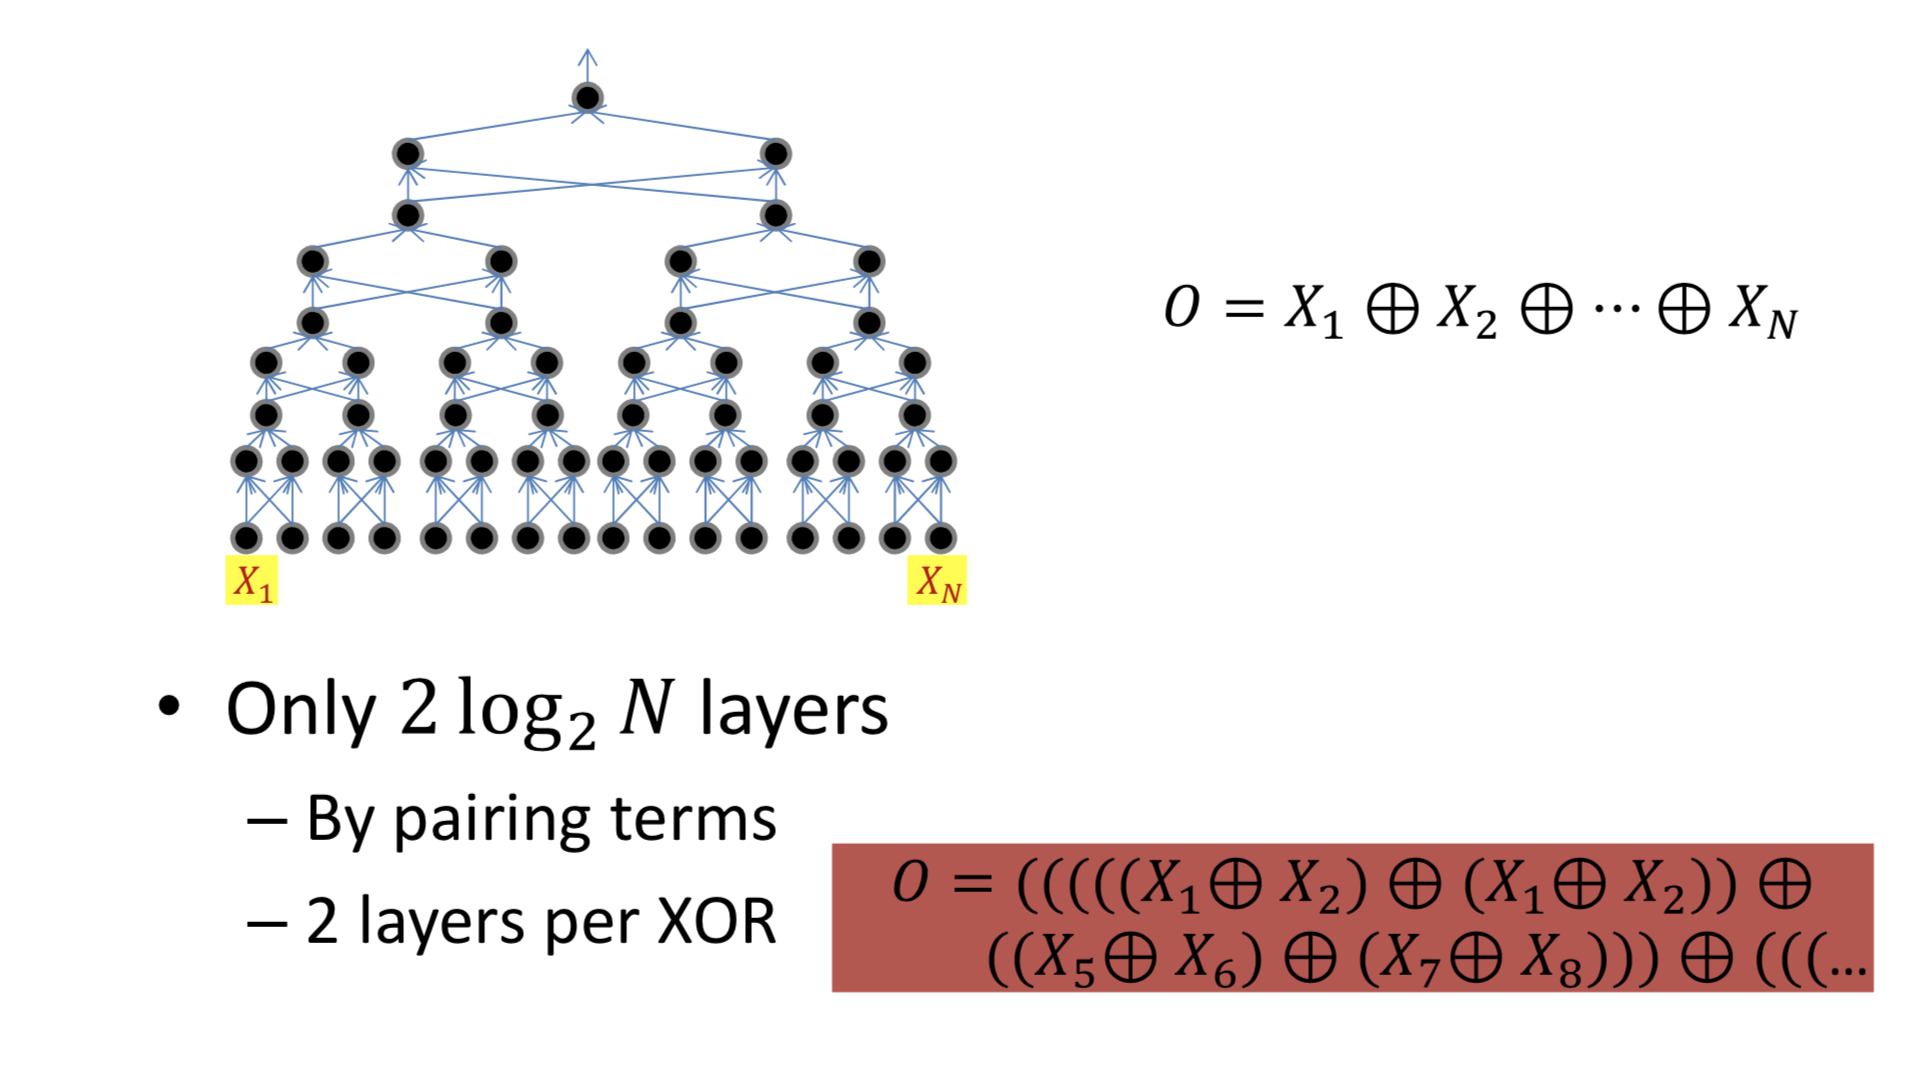
\includegraphics[scale=0.2]{21.png}
	
	Notes: In the worst case, the N-variable XOR method reduces the number of layers by combining the laws.
	
	Conclusion 1.4: Under the worst-case Karnaugh map, using the XOR method, the number of network layers is reduced to $2log_2N$ in a multi-layer perceptron network. \\ 
	
	
	\begin{itemize}
		\item In the worst case, specify the K+1 layer: the trade-off between the number of layers and the number of neurons
	\end{itemize}
	
	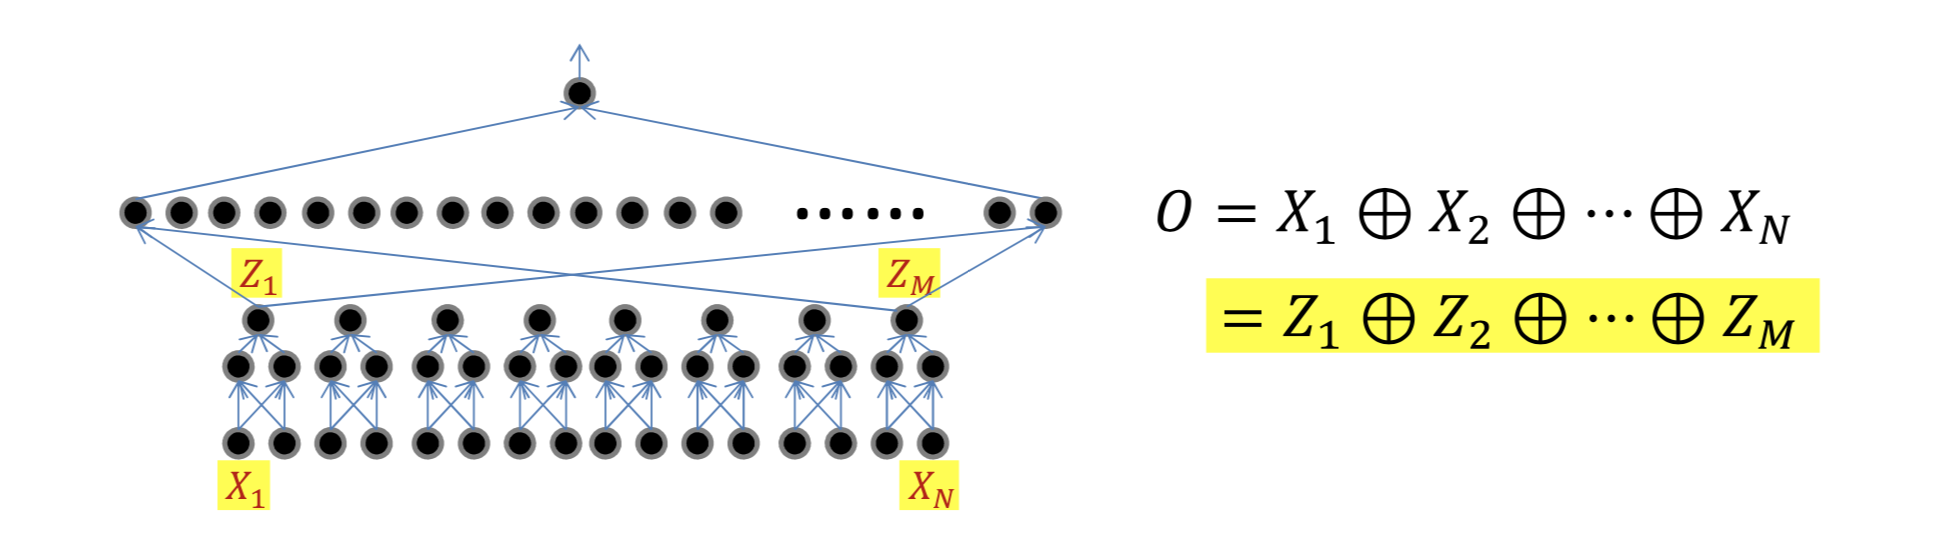
\includegraphics[scale=0.2]{22.png}
	
	Notes: Weigh the number of layers and the number of neurons, specify the K+2 layer, which is equivalent to the pre-K layer XOR method, and the K+1 layer Karnaugh map method. \\
	
	Conclusion 1.5.1: Under the specified k+2 layer, as of the kth layer, according to the XOR method, the number of neurons = $3\sum_{1}^{k}{\frac{N}{2^i}}$ , at the k+1th layer, according to the Karnaugh map method, the number of neurons = $2^{(\frac{N}{2^i}-1)}$, and the last layer, the number of neurons = 1. That is, the final number of neurons = 3 parts of the sum.
	
	Conclusion 1.5.2: If you want to limit the number of layers before the minimum number of layers, it is inevitable that you need to increase the number of neurons in the subsequent layers exponentially. Otherwise, you will not be able to fully cover all the possibilities of the truth table. Cannot fully fit the specified Boolean operation.
	
	\begin{itemize}
		\item Multilayer perceptron network parameter number
	\end{itemize}
	
	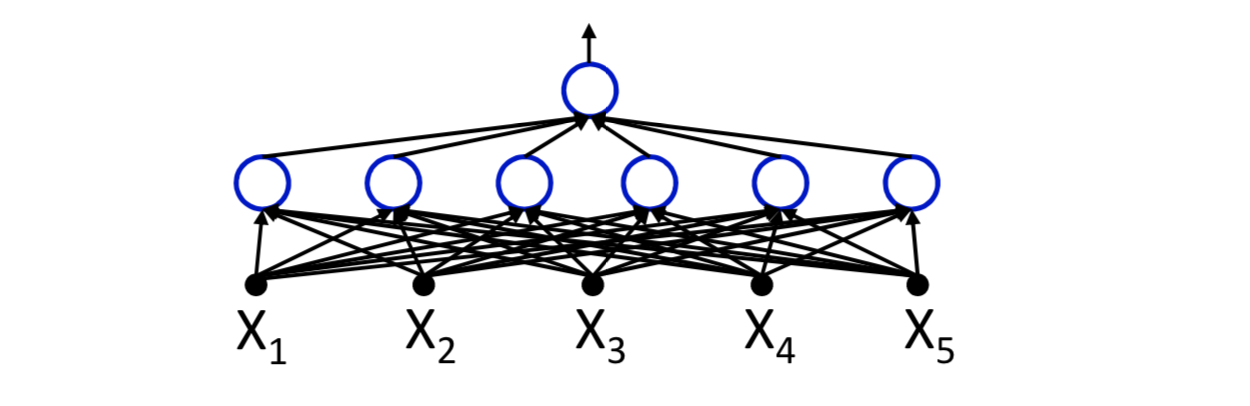
\includegraphics[scale=0.2]{23.png}
	
	Notes: The number of parameters is the number of connections in the network. Very important in hardware and software implementation.
	
	Conclusion 1.6: The number of parameters depends on the number of neurons. If the number of neurons is exponential, the number of parameters of exponential or super-exponential level is inevitably required. \\ 
	
	
	
	\textbf{2. Universal classifier}
	
	Intuitively, a multi-layer perceptron can construct a classification hyperplane combination of any shape by combining multiple decision boundaries. So, is it really only a multi-layer perceptron that implements a universal classifier? Can I use only one layer?
	
	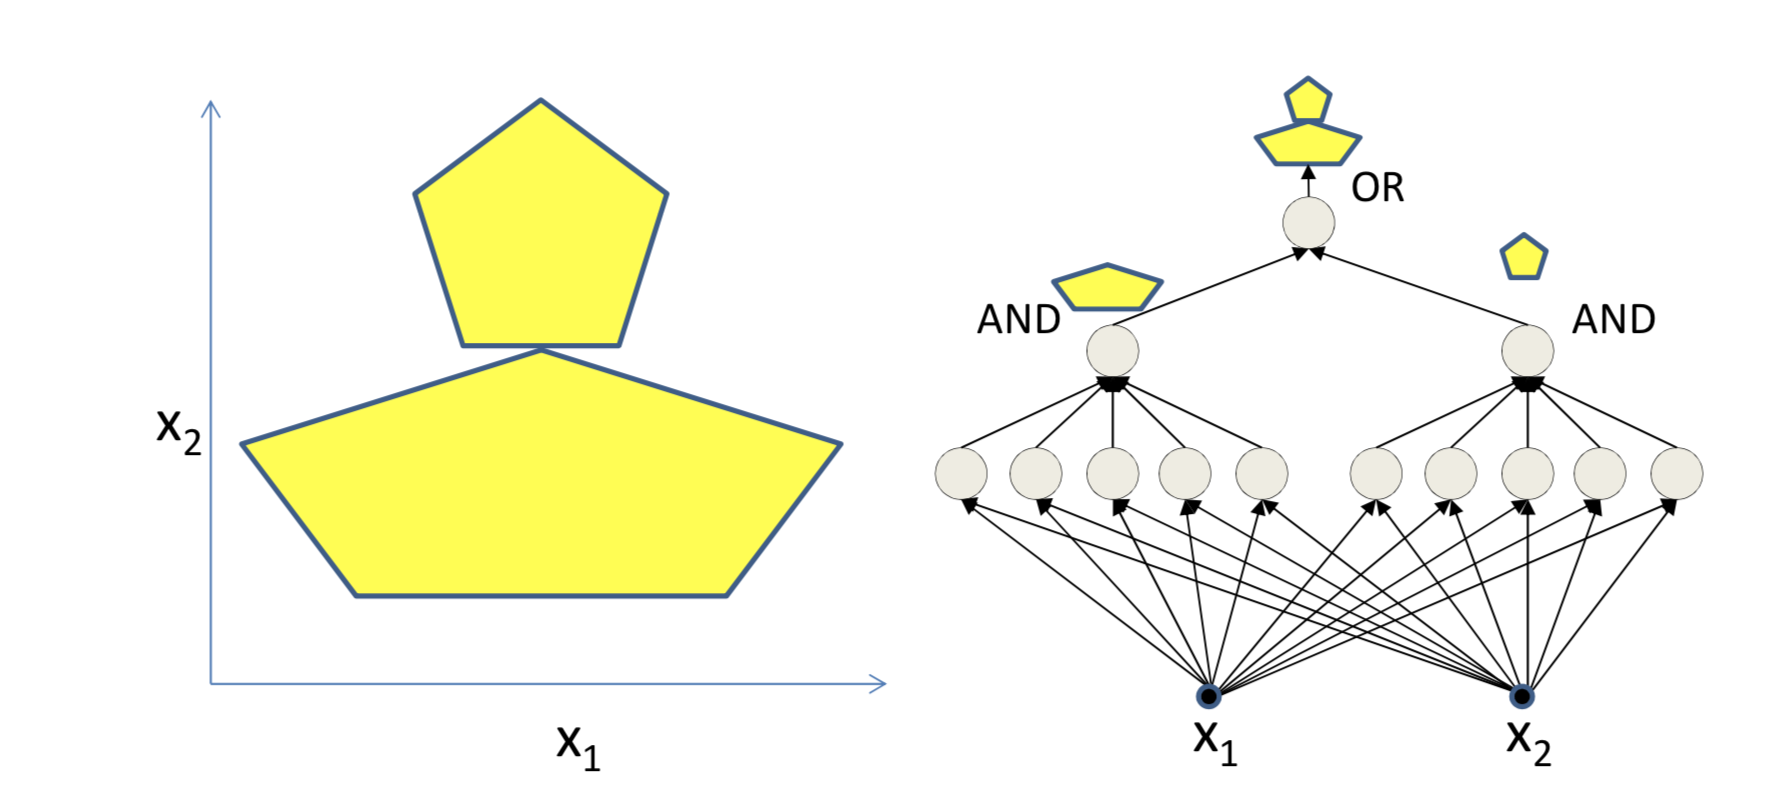
\includegraphics[scale=0.2]{24.png}
	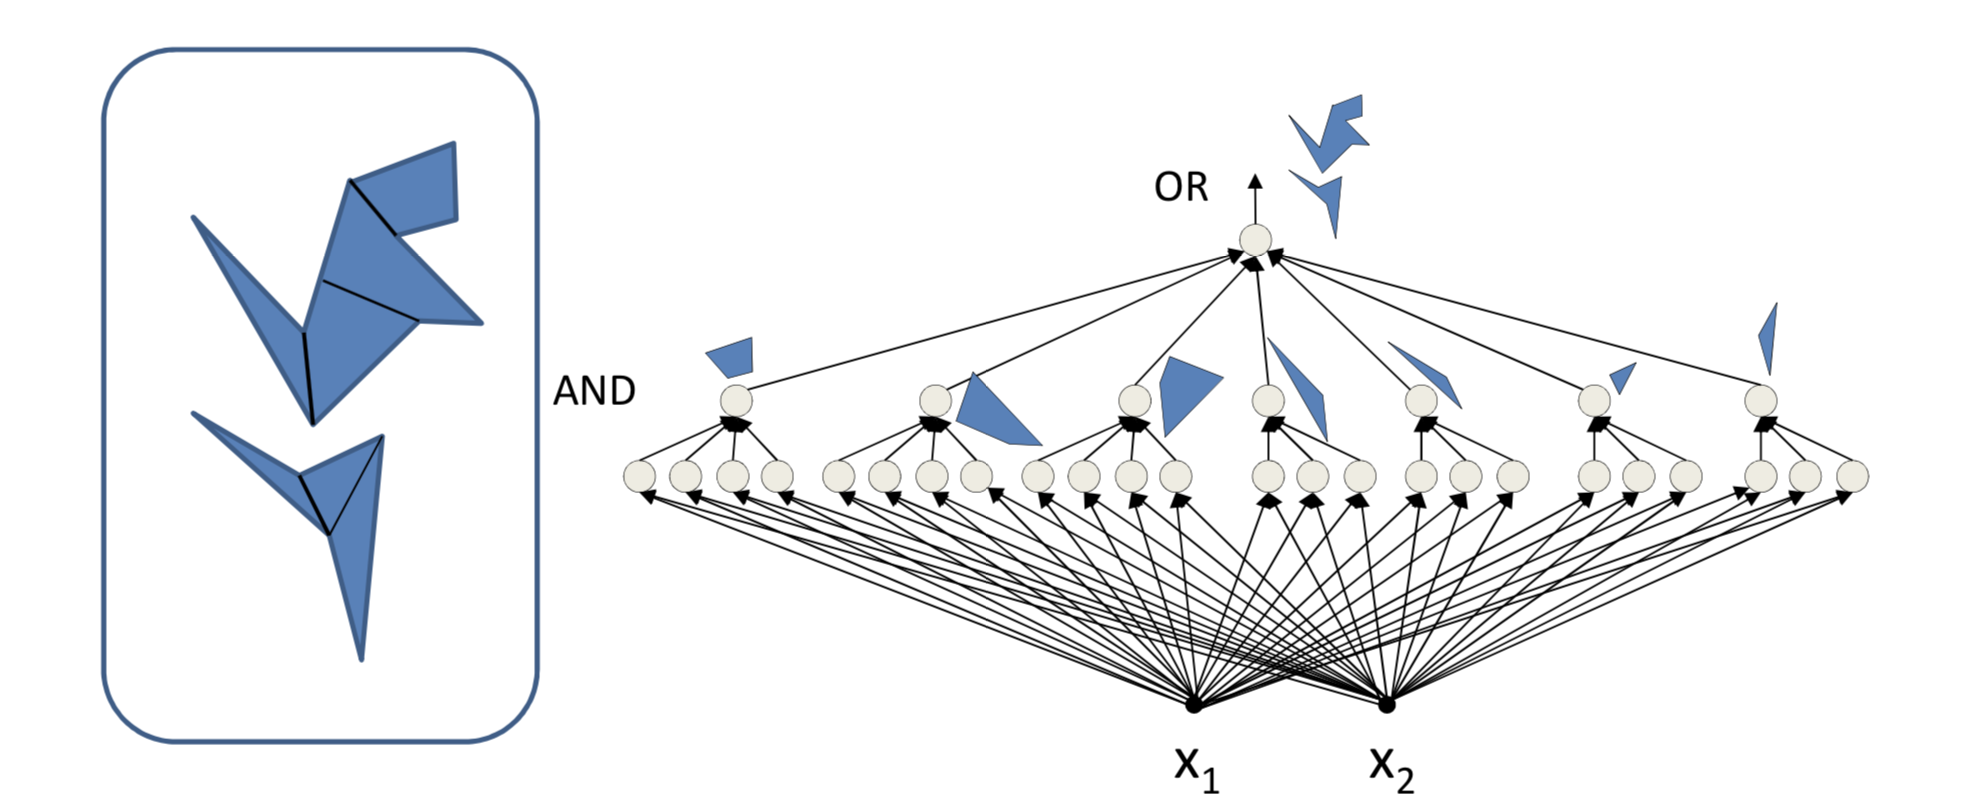
\includegraphics[scale=0.2]{25.png}
	
	\begin{itemize}
		\item A layer of perceptron network: an infinite number of neurons, depending on accuracy
	\end{itemize}
	
	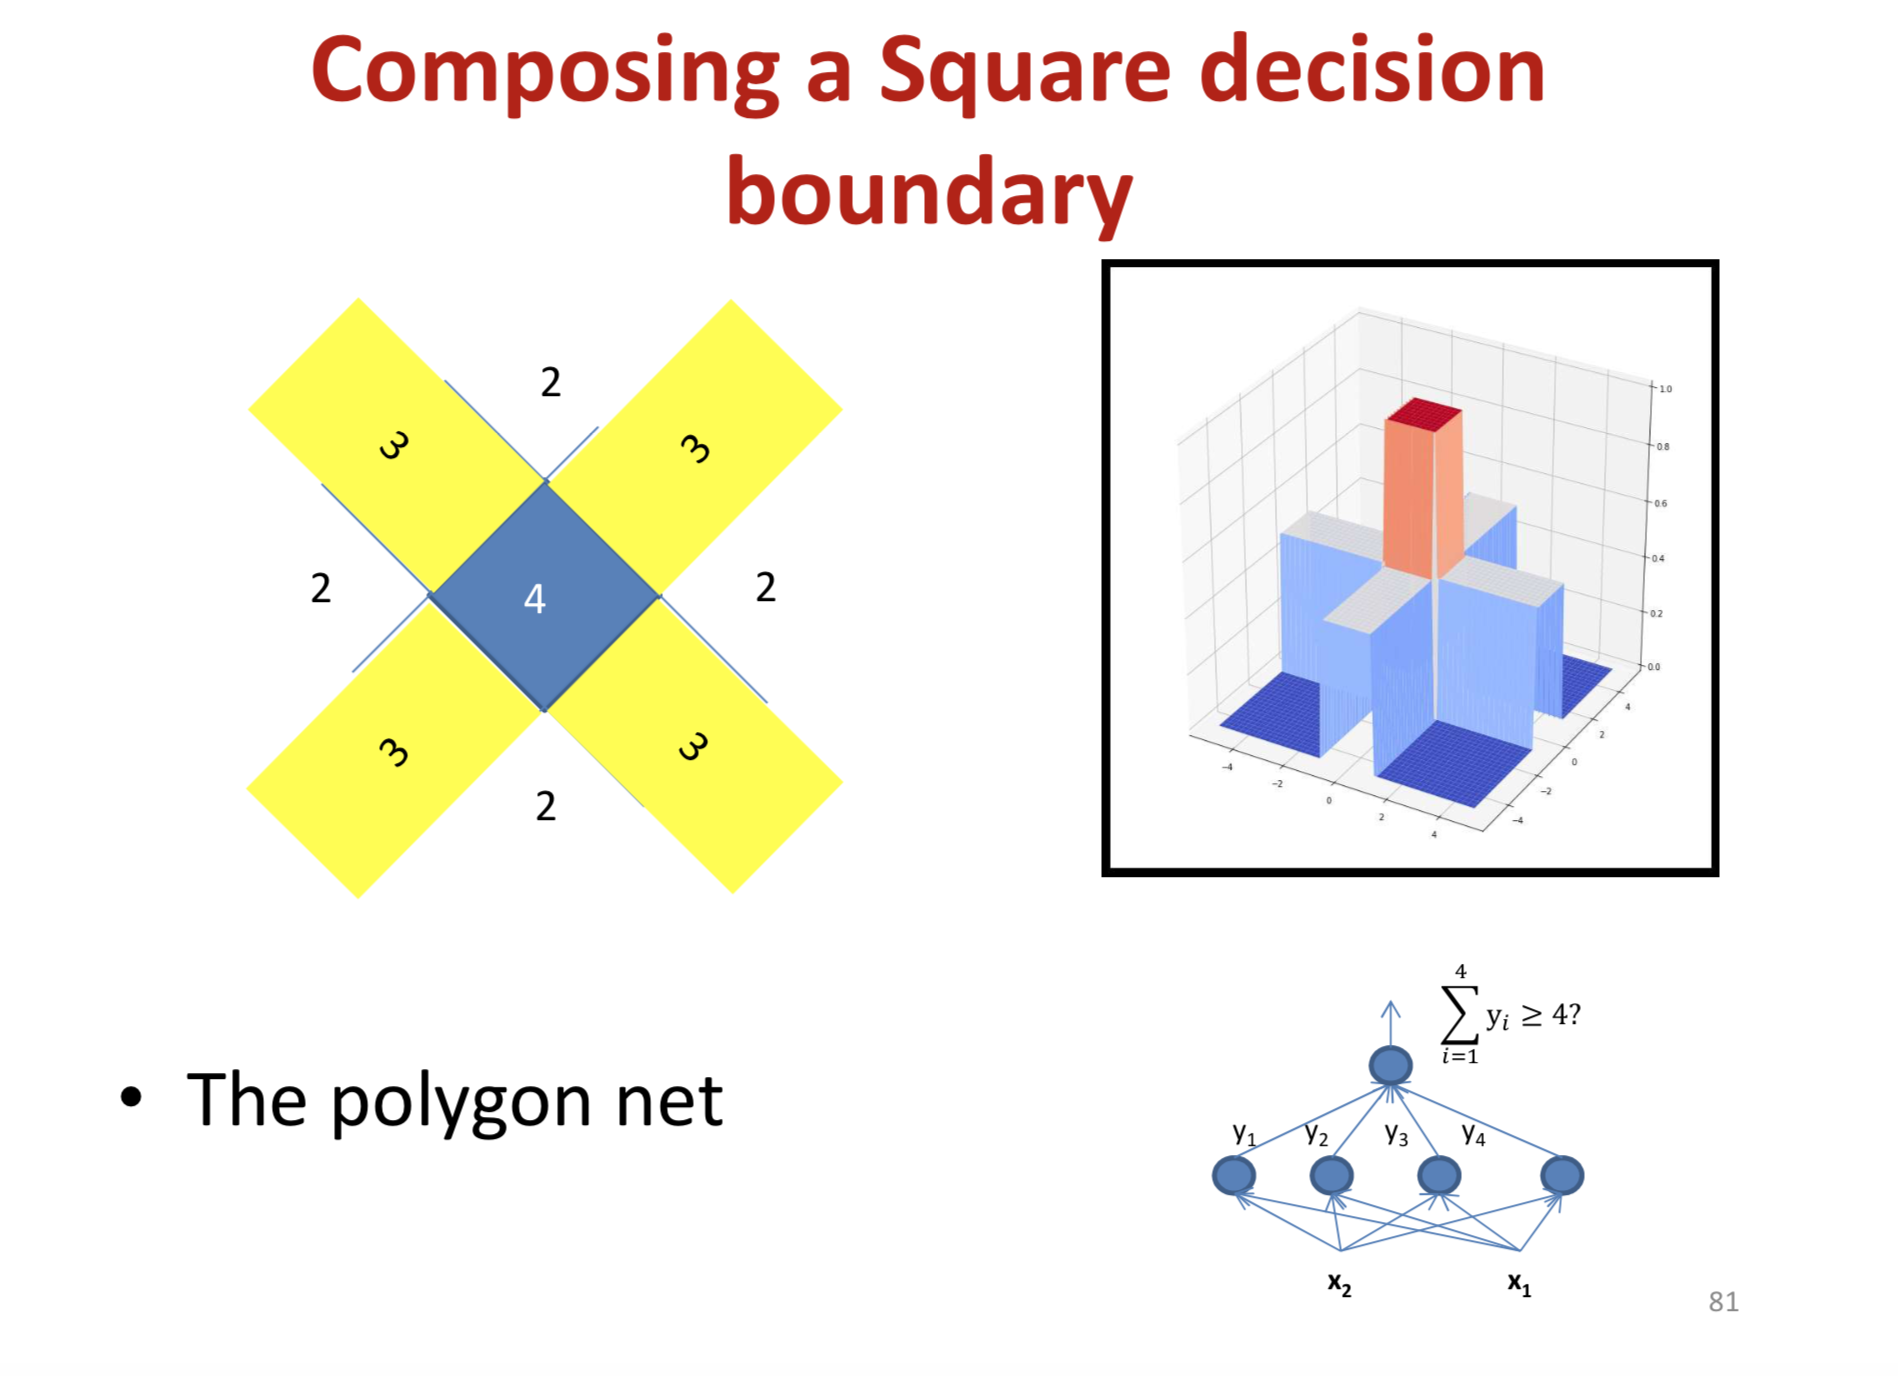
\includegraphics[scale=0.2]{26.png}
	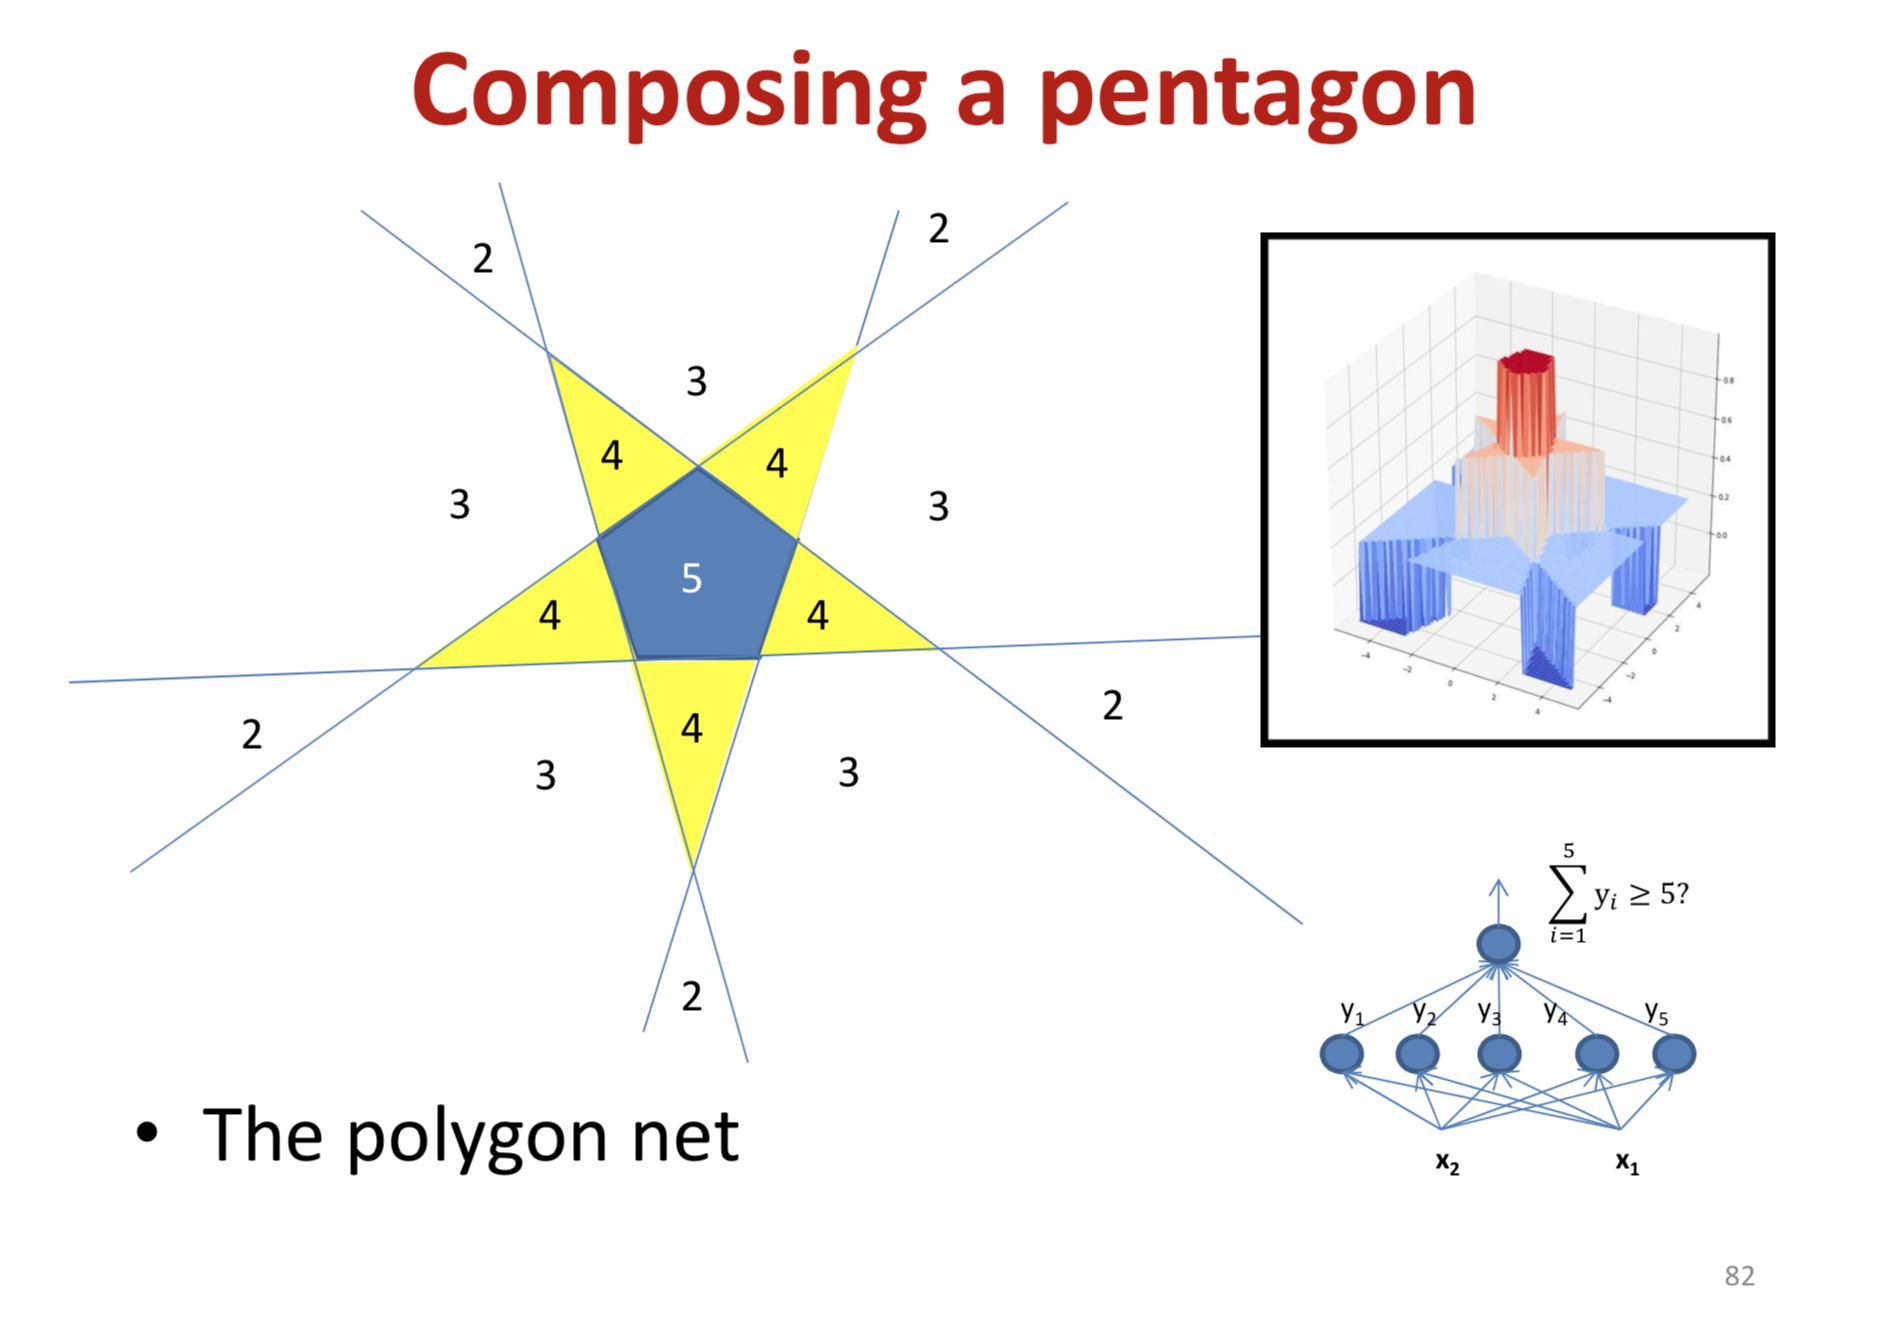
\includegraphics[scale=0.2]{27.png}
	
	Notes: Each neuron corresponds to a decision line, and the value of the central decision surface is the largest, as shown by the black box in the three-dimensional space.
	
	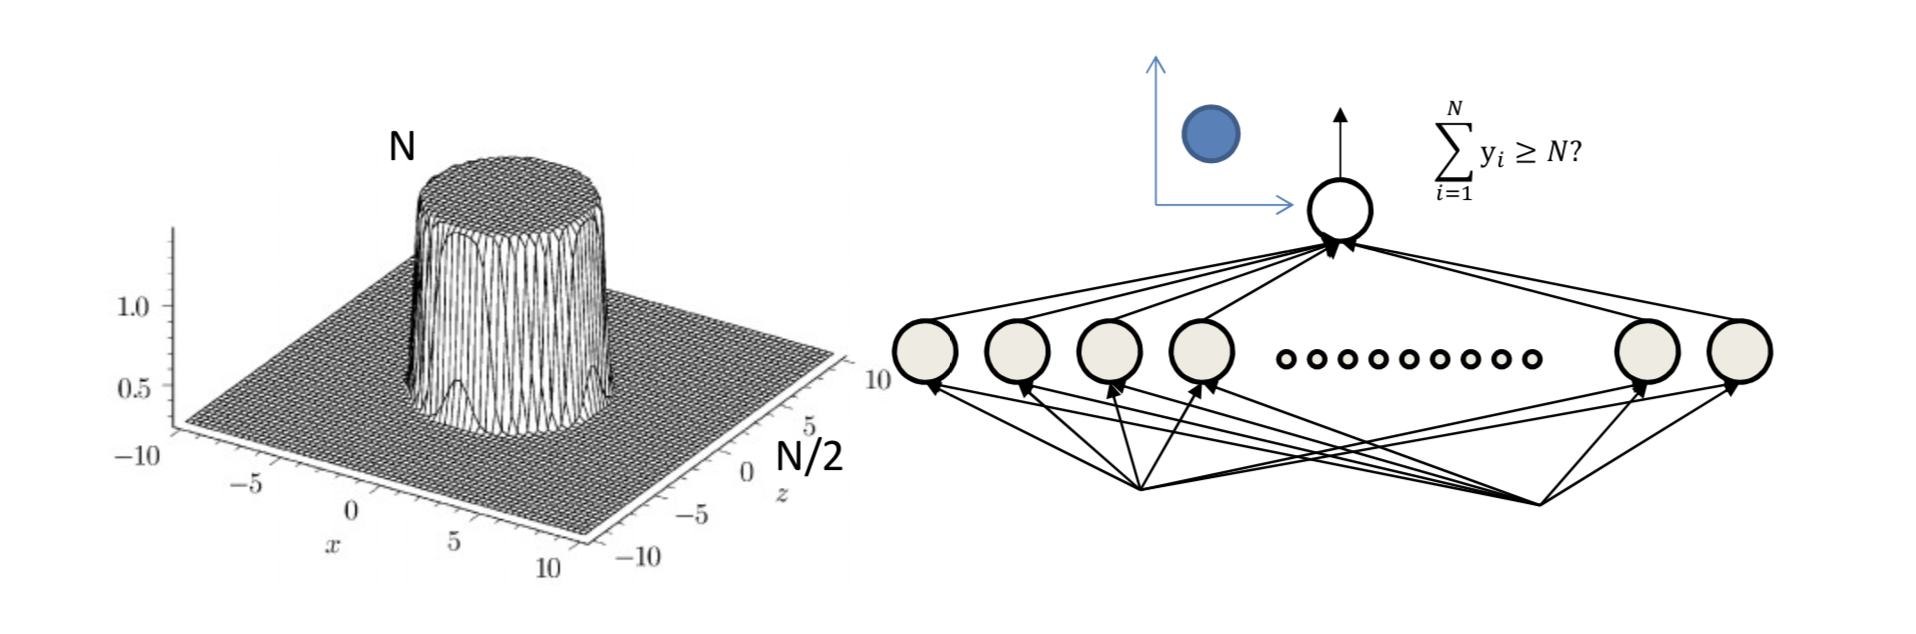
\includegraphics[scale=0.2]{28.png}
	
	Notes: It is always possible to make the center close to the cylinder by continuously increasing the decision line. The center value is N and quickly drops to N/2. Note that the cylinder itself can be located anywhere, depending on the decision line position of the combination.
	
	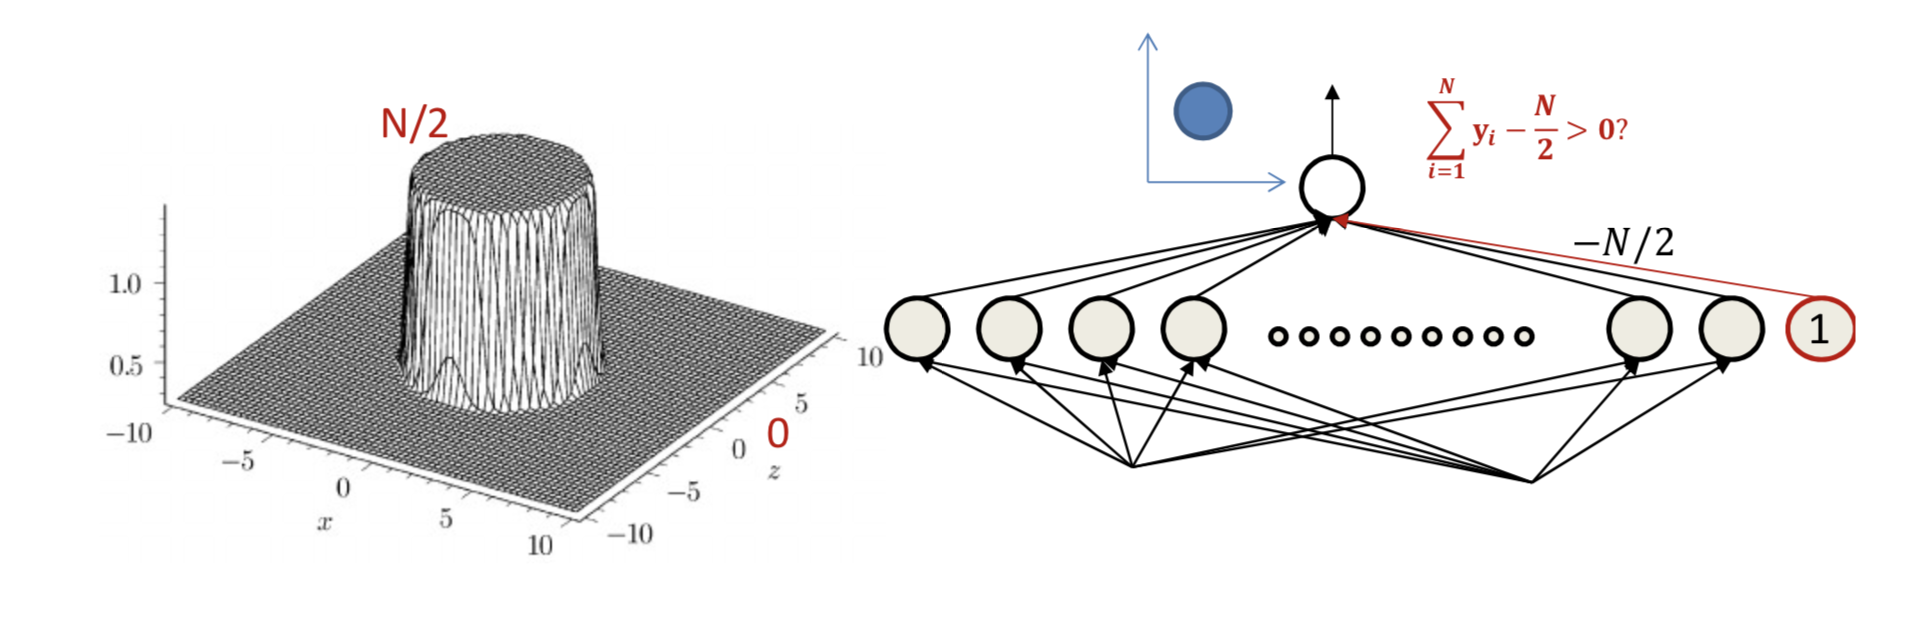
\includegraphics[scale=0.2]{29.png}
	
	Notes: Change the center of the cylinder by adding a neuron 1.
	
	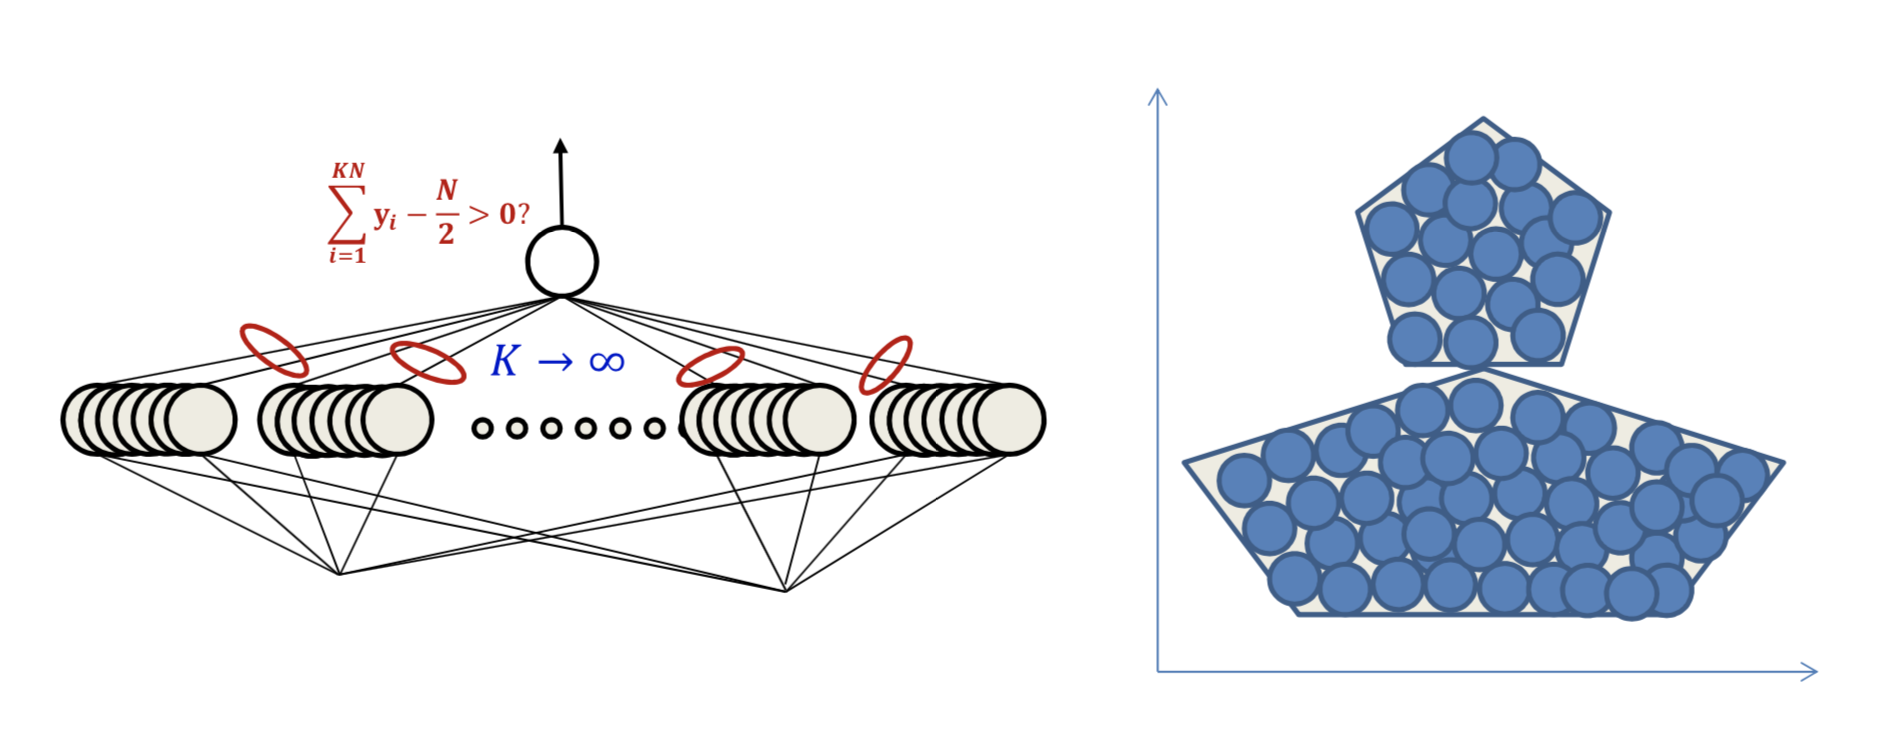
\includegraphics[scale=0.2]{30.png}
	
	Notes:Infinitely filled, fits the decision surface of any shape. Accuracy can be specified
	
	Conclusion 1.1: The perceptron network of a single layer of infinitely many neurons can fit any decision surface, but a deep network requires fewer neurons to achieve its goal.
	
	
	\begin{itemize}
		\item Multilayer perceptron network, choose the optimal depth: the infinity of single-layer network neurons, requires the use of multi-layer perceptron to solve the problem
	\end{itemize}
	
	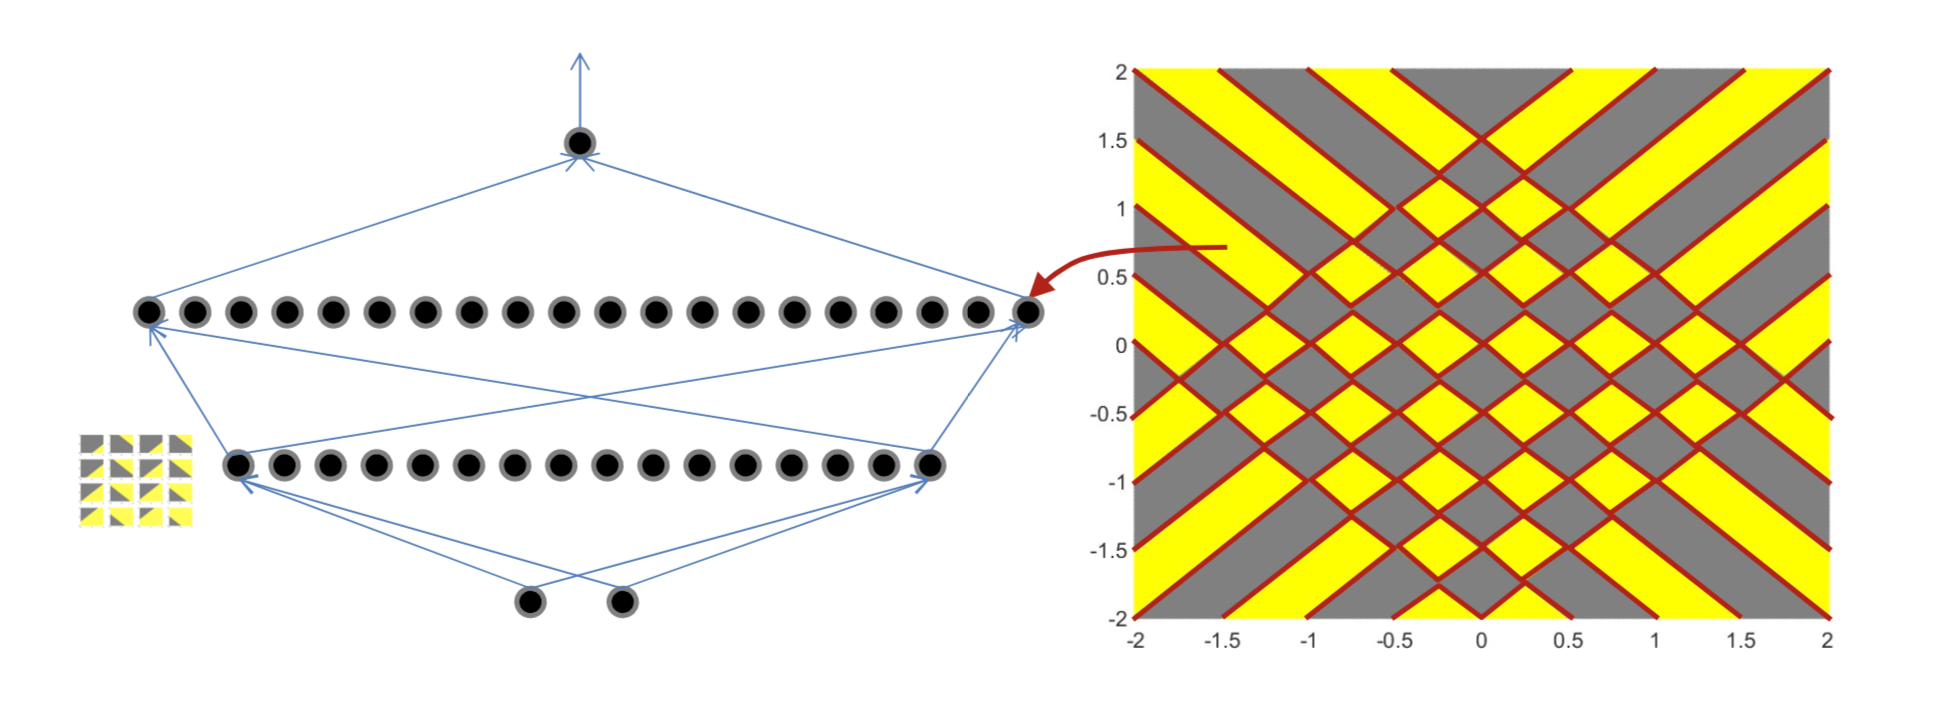
\includegraphics[scale=0.2]{31.png}
	
	Notes: Karnaugh map: two hidden layer networks: the first layer represents 16 decision lines (2 original inputs, which can be drawn freely in the plane), and the 2nd layer represents 40 decision surfaces (black squares).
	
	
	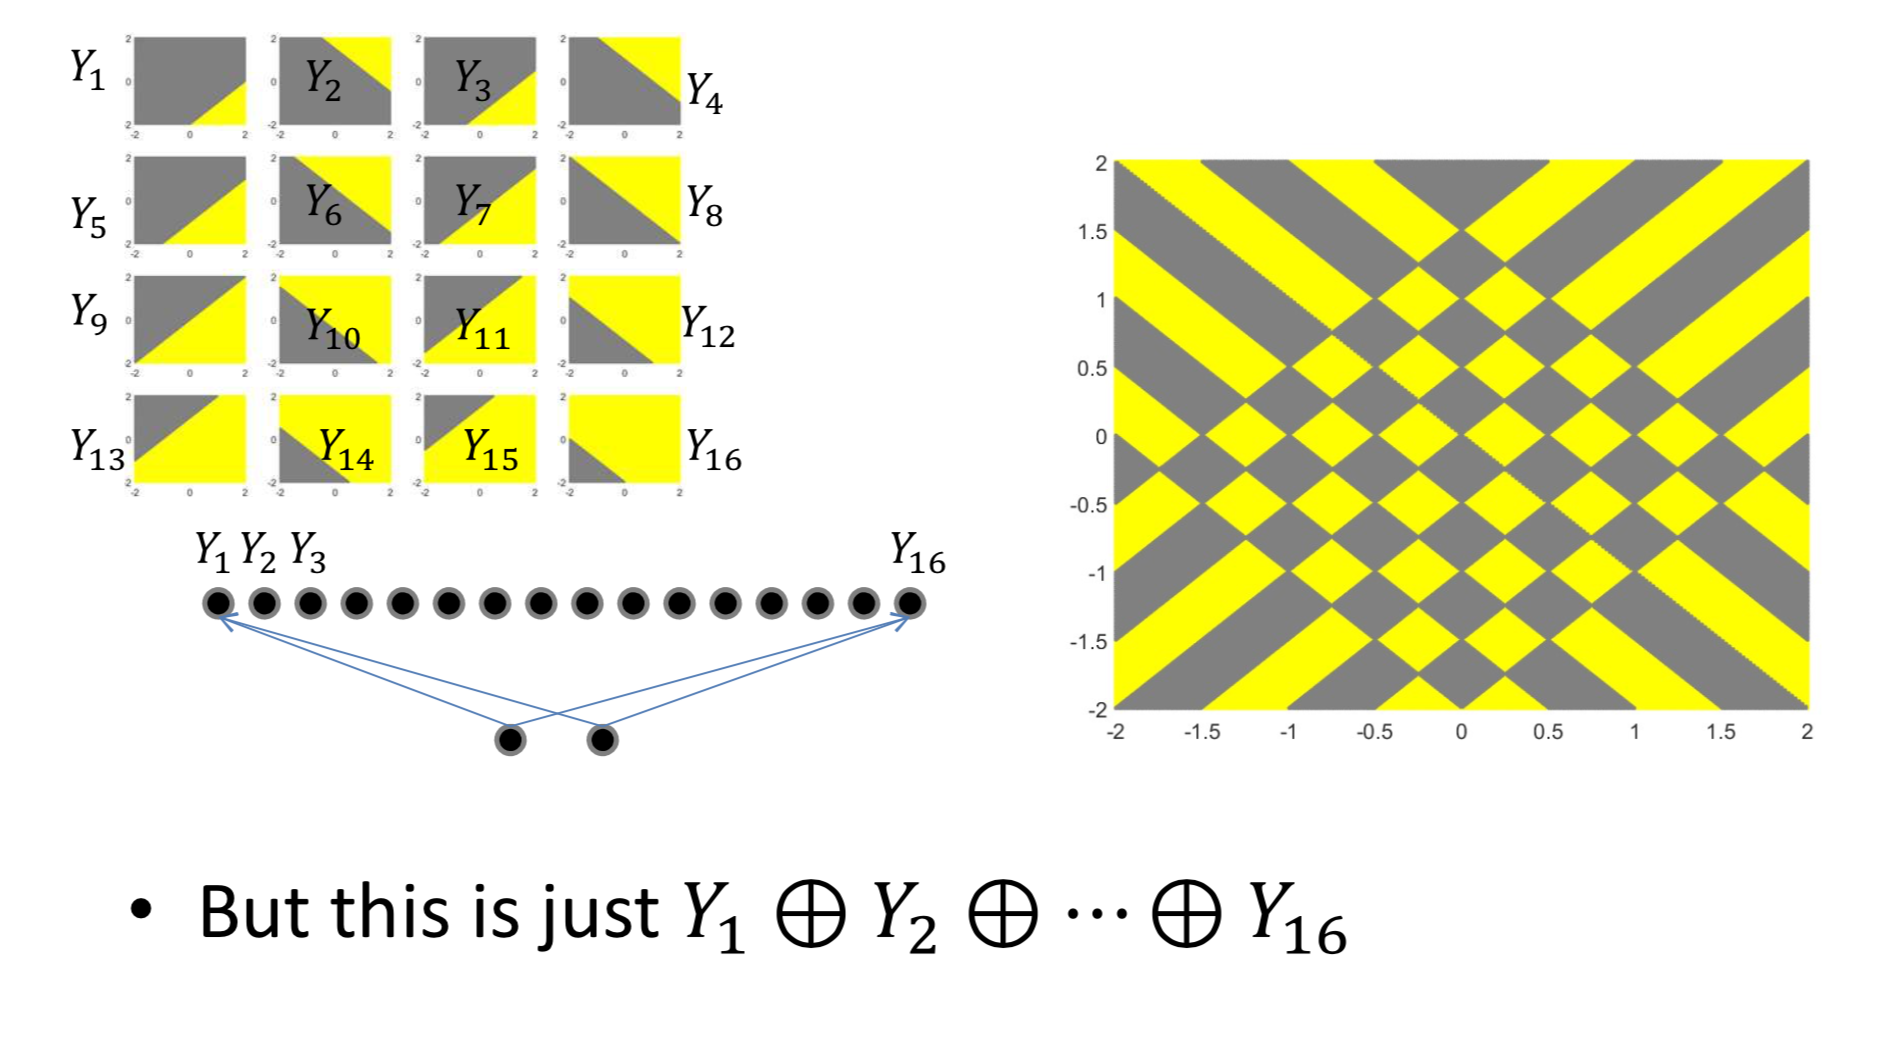
\includegraphics[scale=0.2]{32.png}
	
	Notes: XOR law: Several hidden layer networks: Layer 1 represents 16 decision lines, and subsequent layers represent two or two XOR (16 inputs, 15 XOR operations, totaling $15*3$ neurons). 
	
	Conclusion 2.1: In the two hidden layer networks, the second layer requires $(N+2)^2/8$ neurons. Although from the first hidden layer, the number of neurons is not exponential. But compared to the input layer (two-dimensional variable), the number of neurons is exponentially increasing.
	
	Therefore, as the input layer dimensions increase, the number of shallow network neurons constructed in a Karnaugh map manner increases exponentially. However, the network constructed by the XOR law has little effect, because the number of neurons in its subsequent layer depends only on the number of decision lines in the first layer. \\
	
	\textbf{3. Universal continuous functionr}
	
	Lecture1 has discussed the univariate function fitting. For multivariate high-dimensional input, the fitting idea of the general classifier can be used to fit the cylinder. \\  \\ \\ \\ \\ \\
	
	
	\begin{itemize}
		\item Single variable input, pulse function
	\end{itemize}
	
	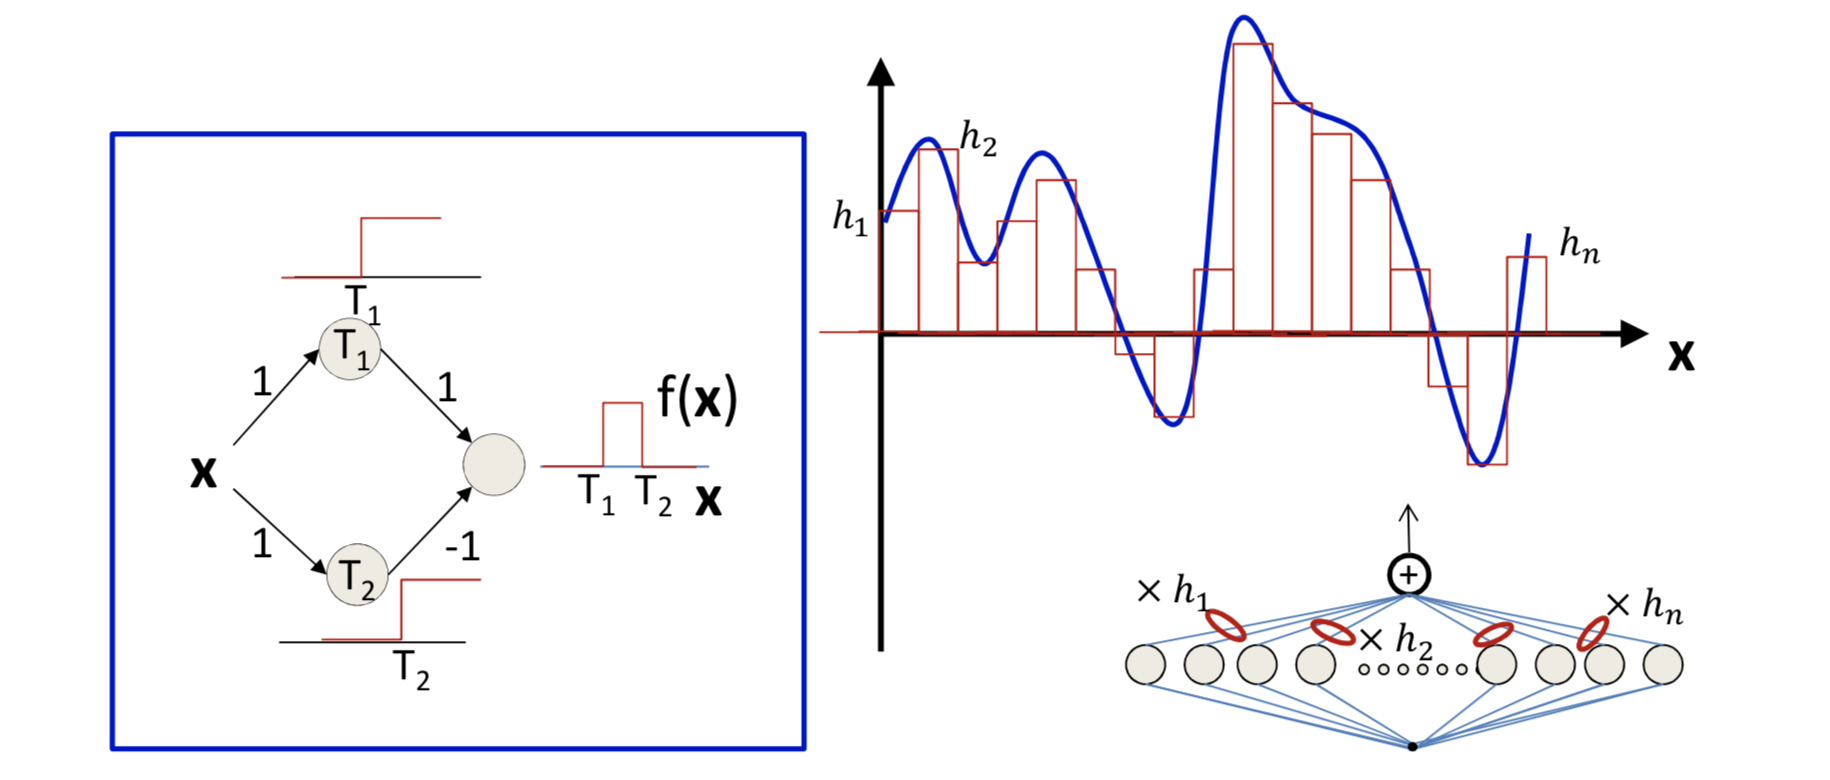
\includegraphics[scale=0.2]{33.png}
	
	\begin{itemize}
		\item Multivariate input, cylinder partitioning: similar to the discussion of general classifiers
	\end{itemize}
	
	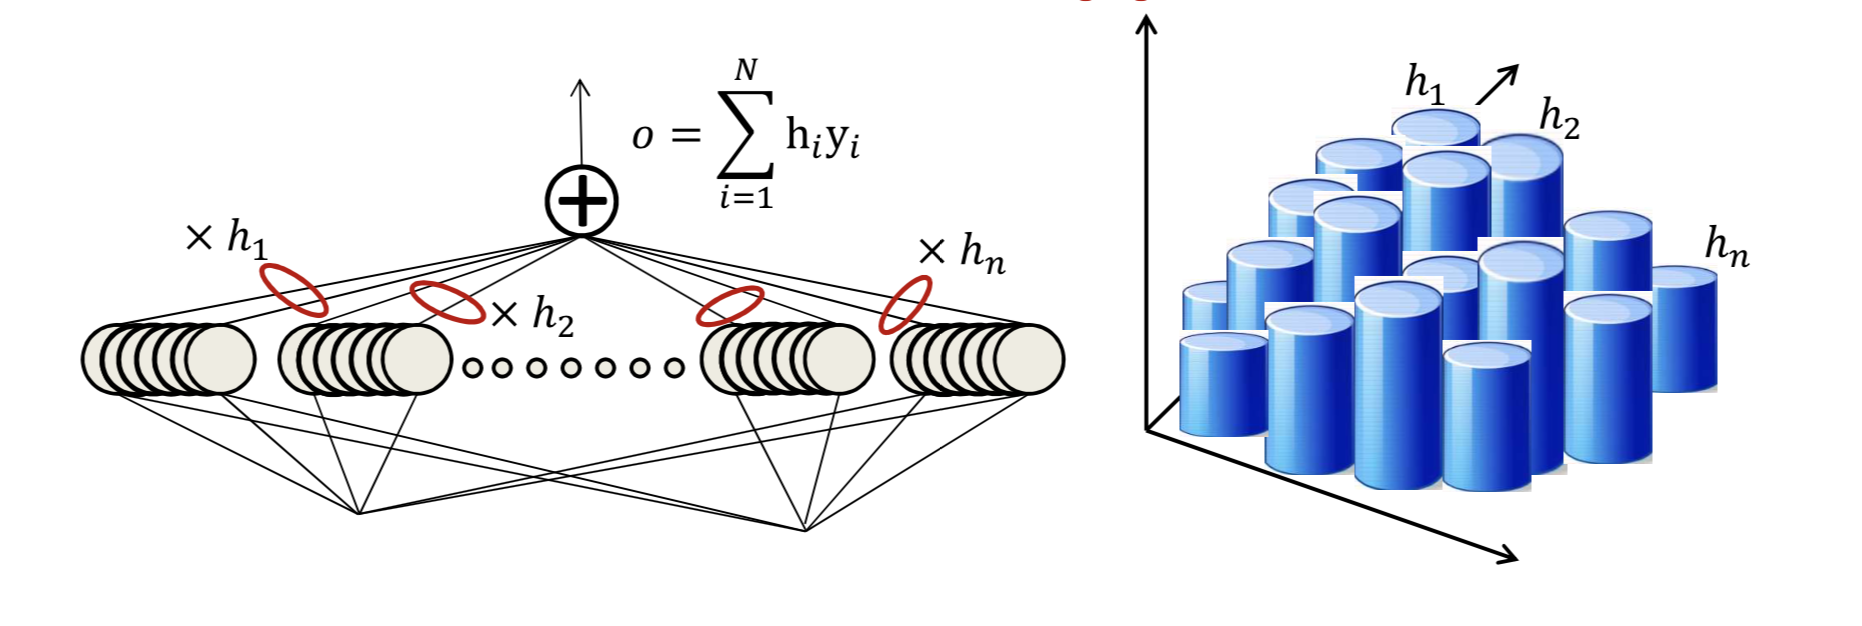
\includegraphics[scale=0.2]{34.png} \\
	
	\textbf{3. Adequacy of neural network architecture: Neural networks adapted to generic functions must have sufficient capacity}
	
	\begin{itemize}
		\item Use threshold activation function
	\end{itemize}
	
	In the discussion of the general classifier, if the first hidden layer replaces 16 neurons with 8 neurons, it will result in insufficient pattern capture. The second hidden layer could not be lost in the first layer anyway.
	
	Similarly, if the second hidden layer replaces 40 neurons with 16 neurons, it will also miss the decision surface of the square or stripe, losing the pattern.
	
	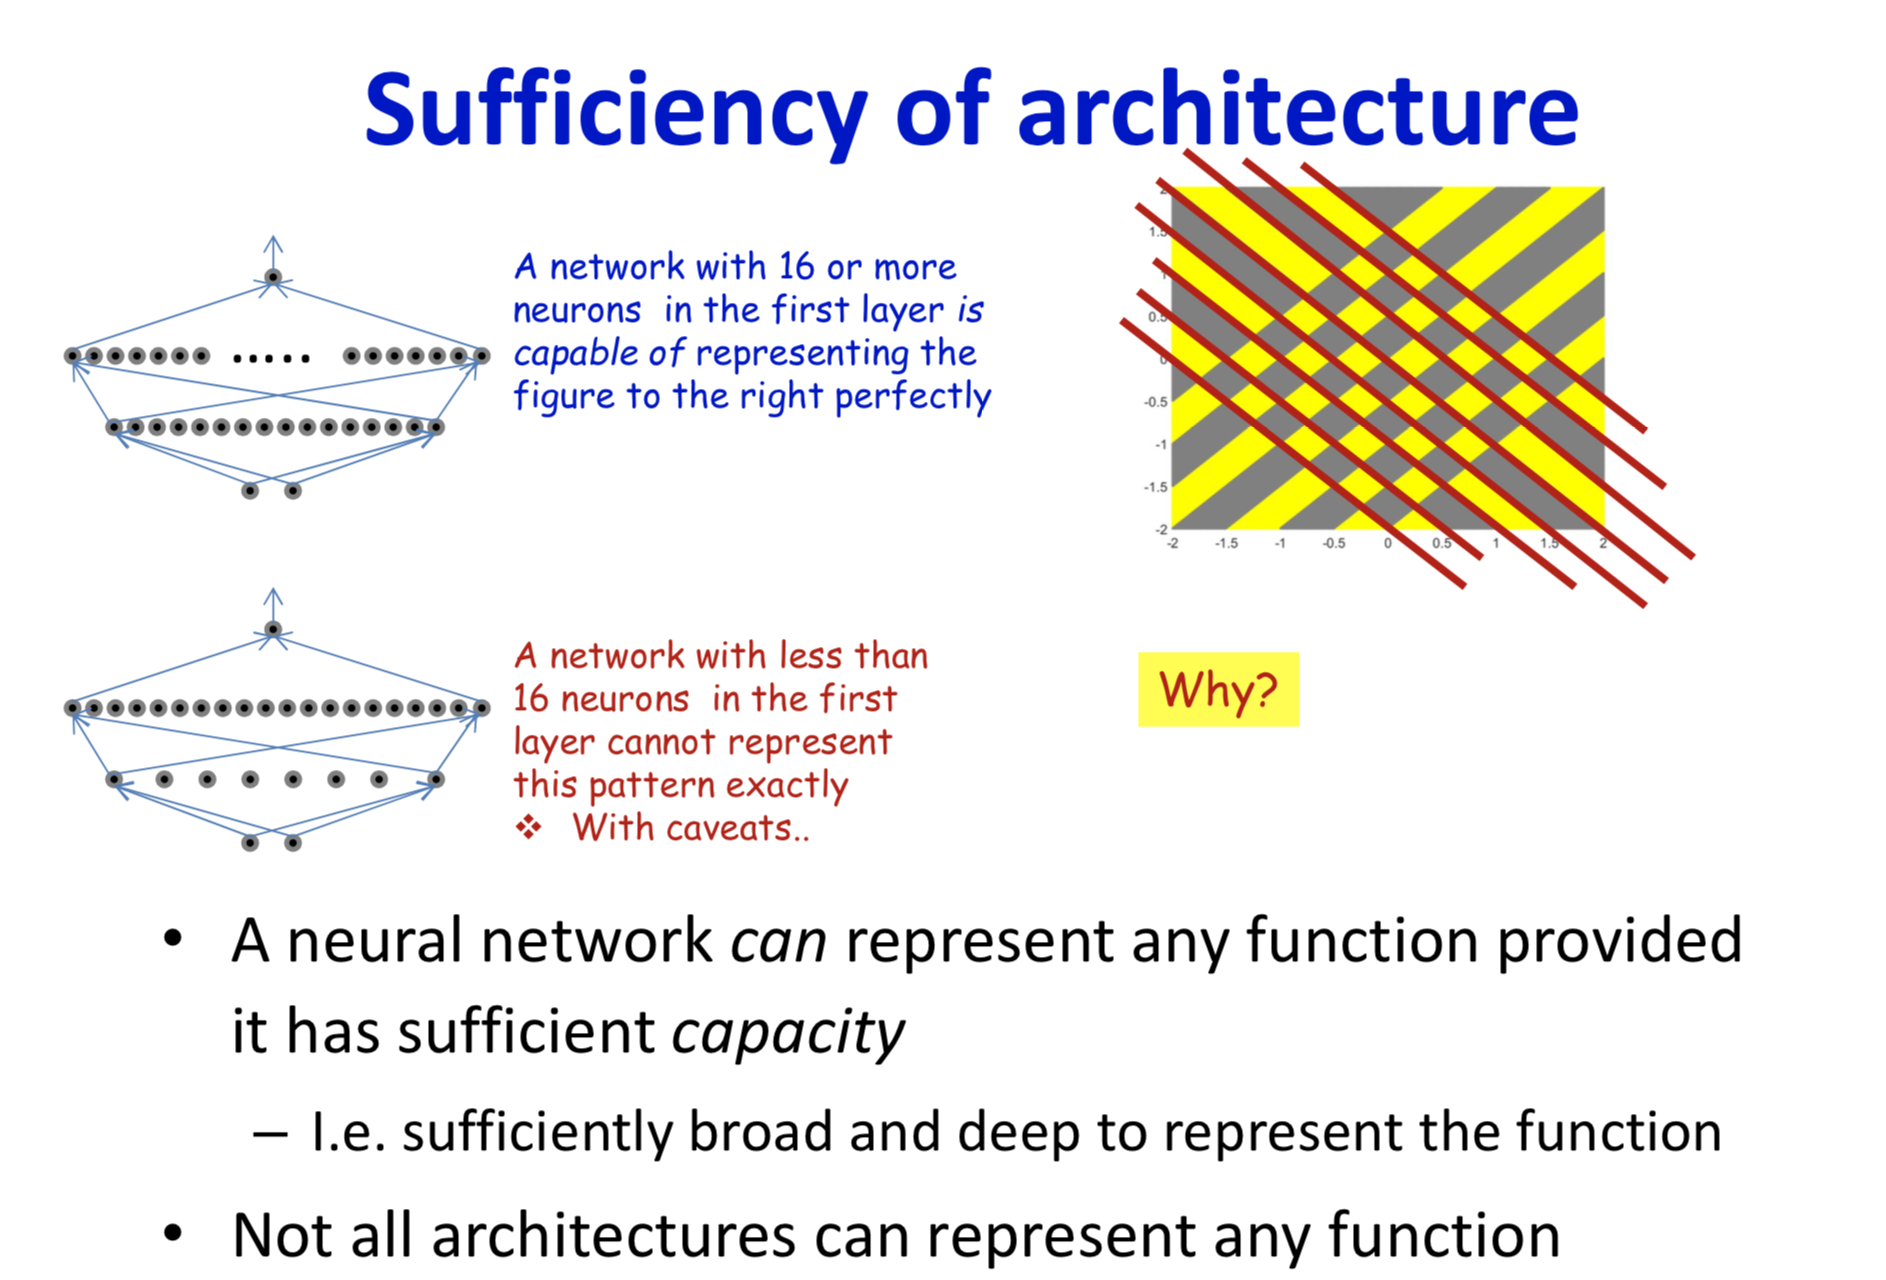
\includegraphics[scale=0.2]{35.png}
	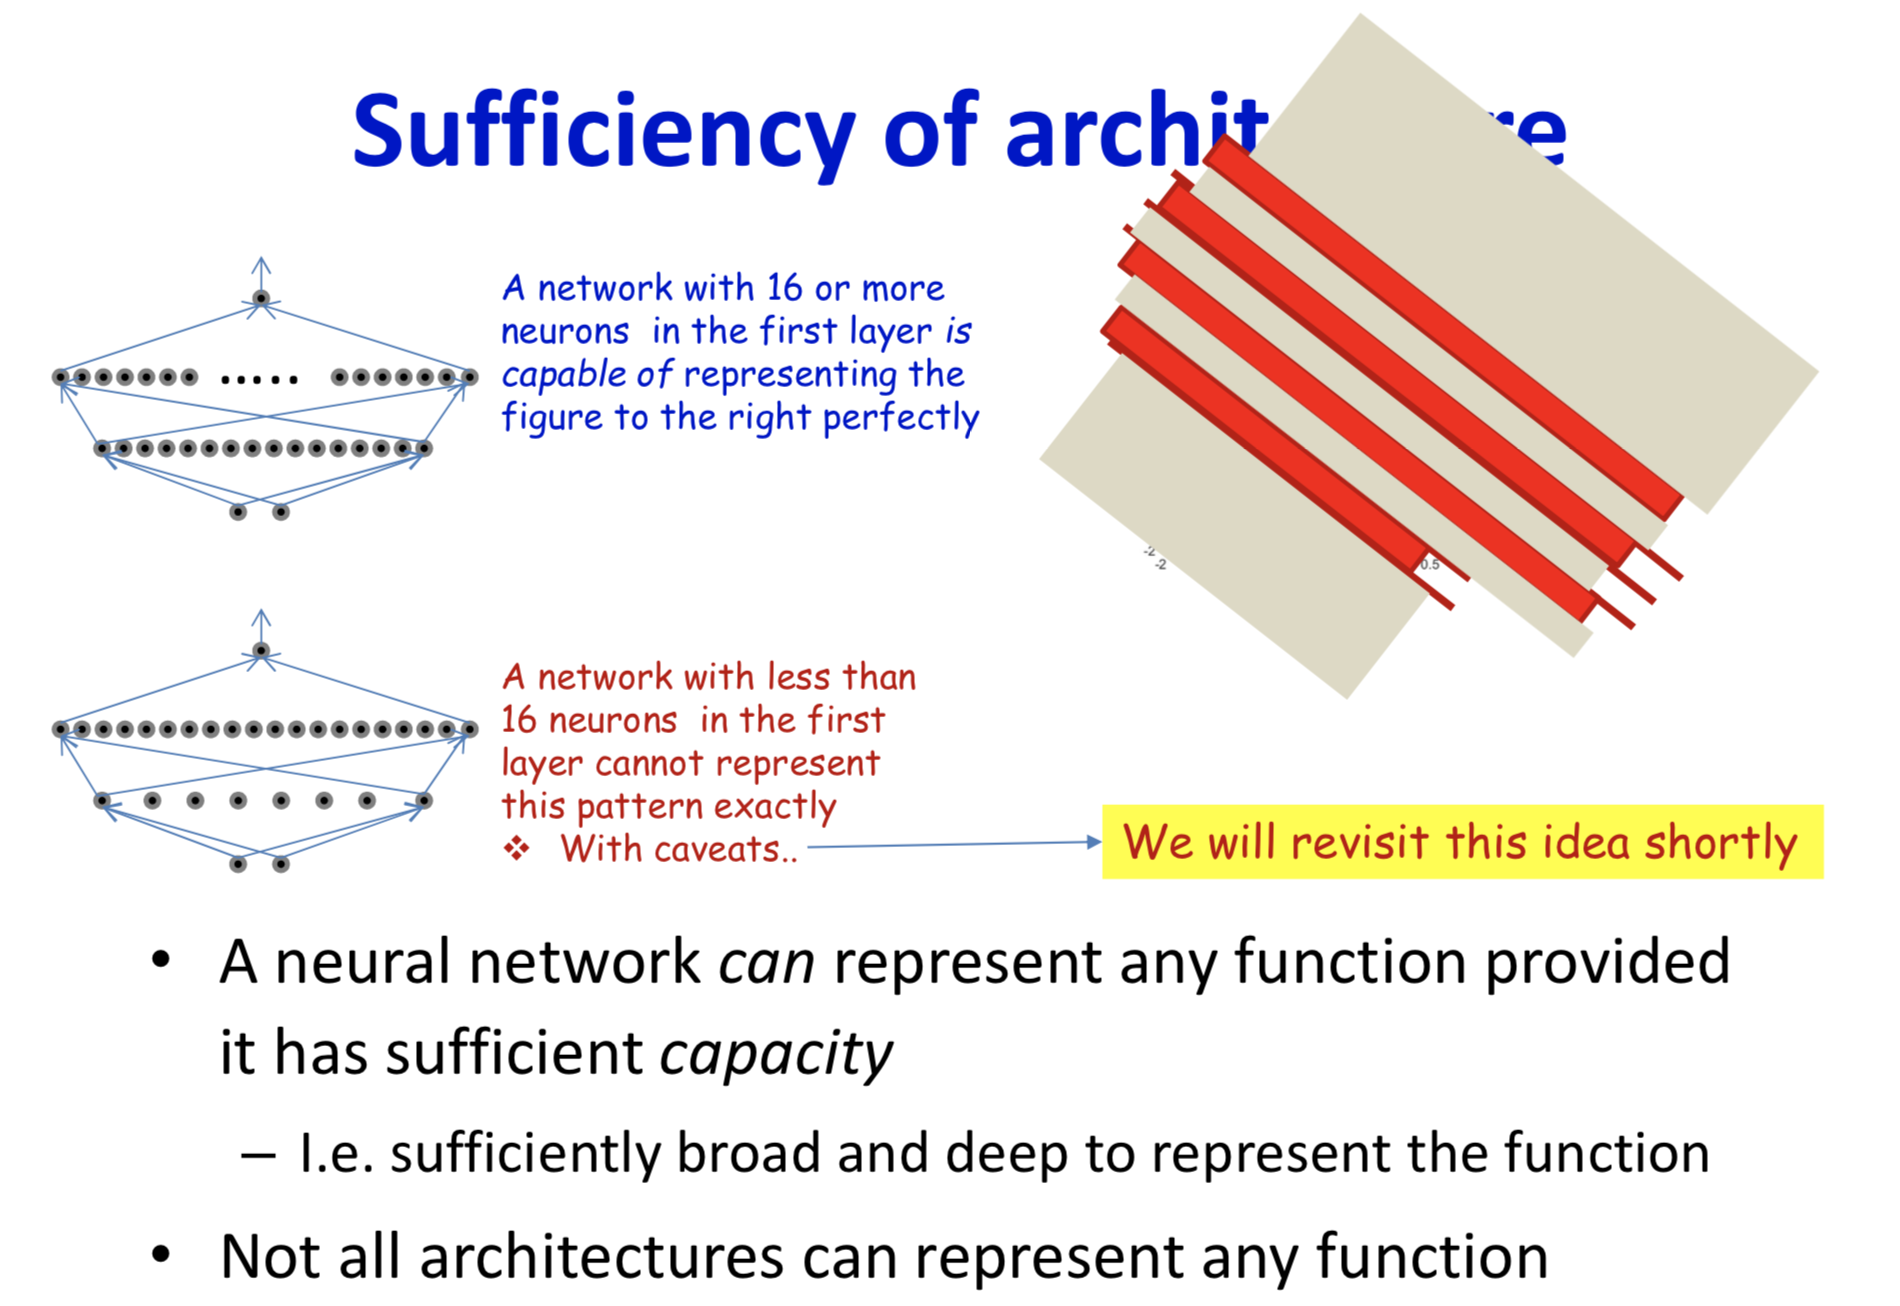
\includegraphics[scale=0.2]{36.png}
	
	Notes: Lost the decision line from the top right-bottom decision line
	
	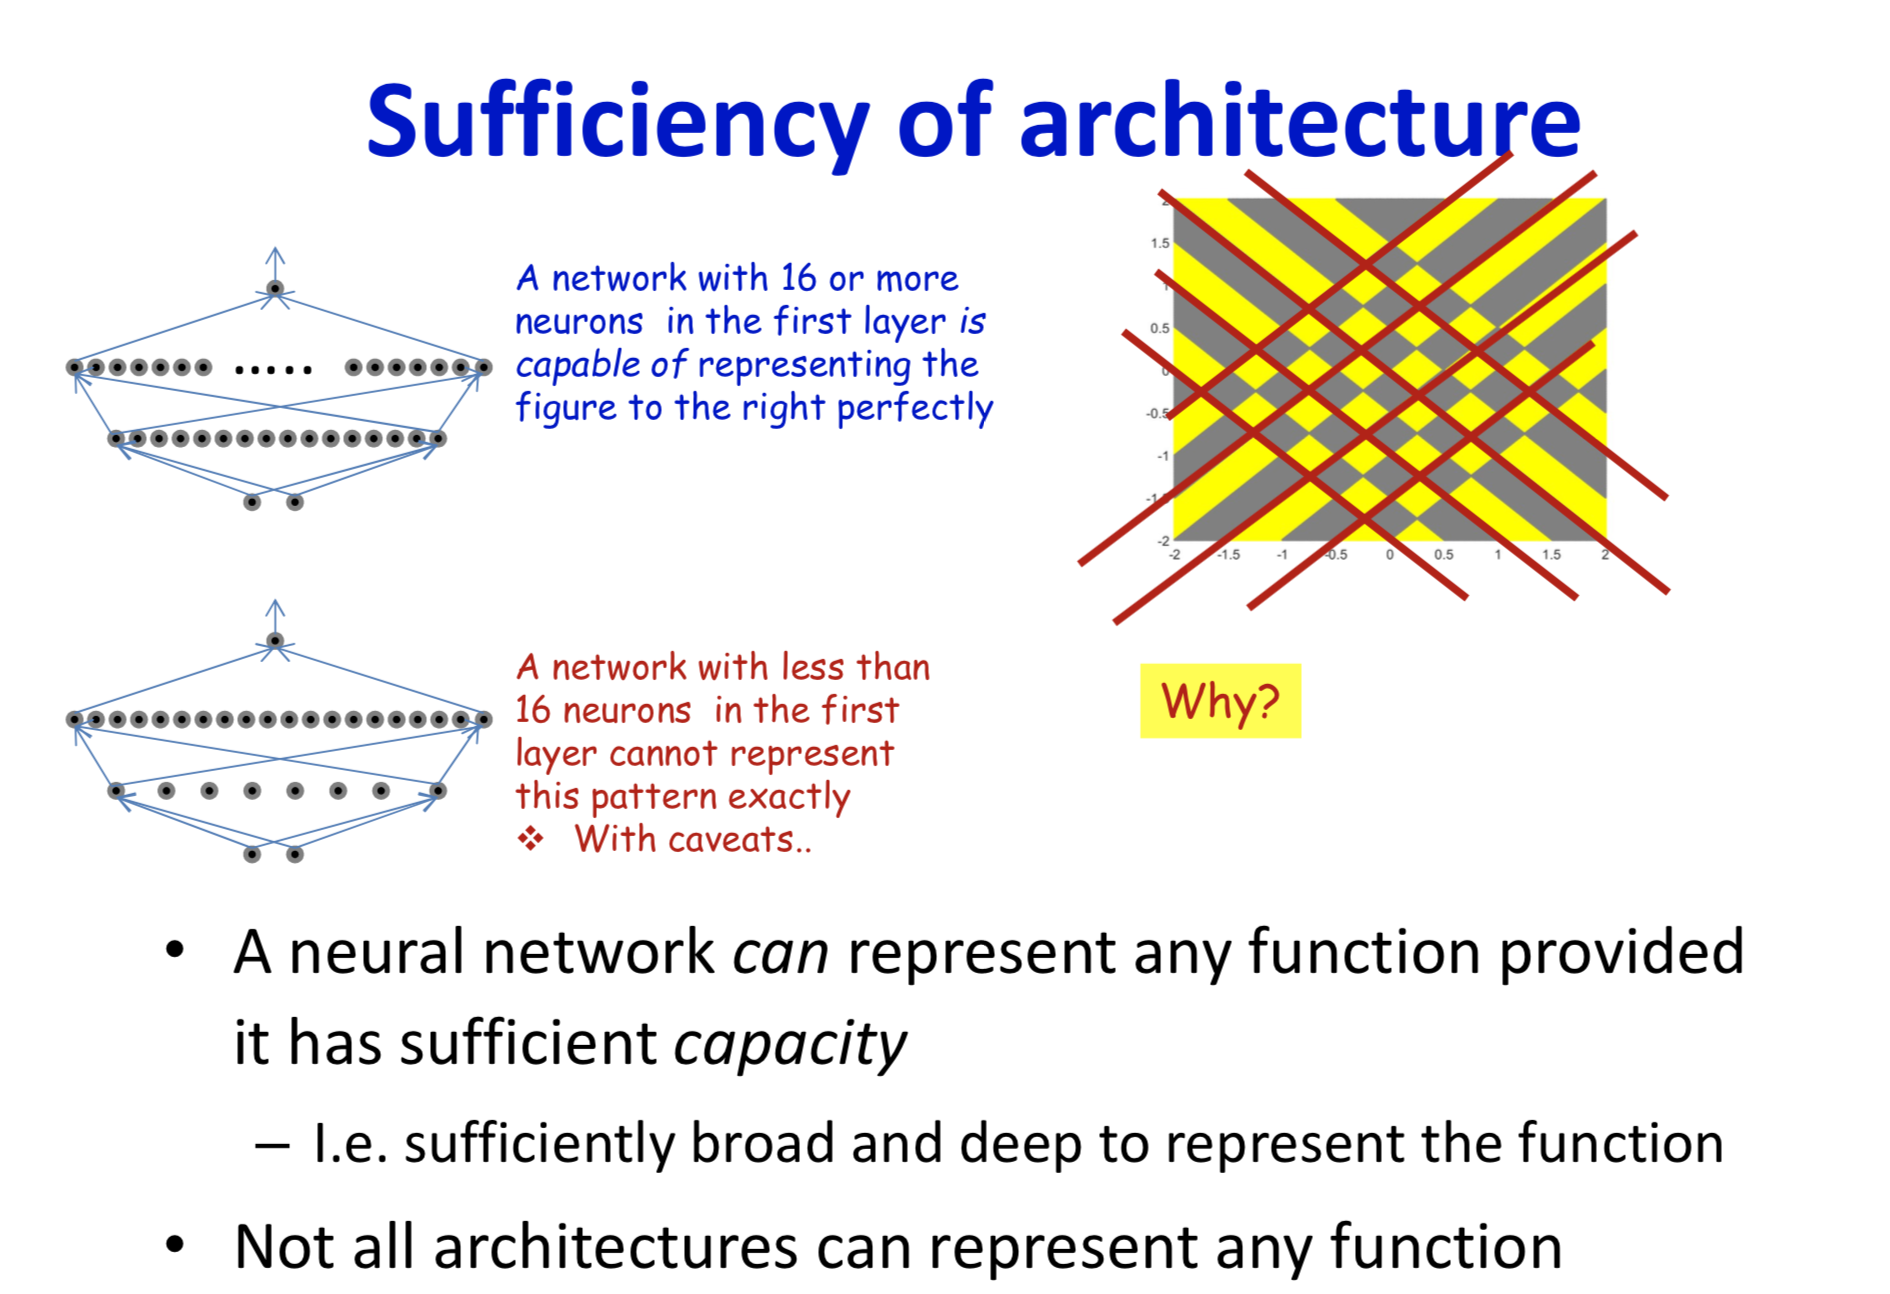
\includegraphics[scale=0.2]{37.png}
	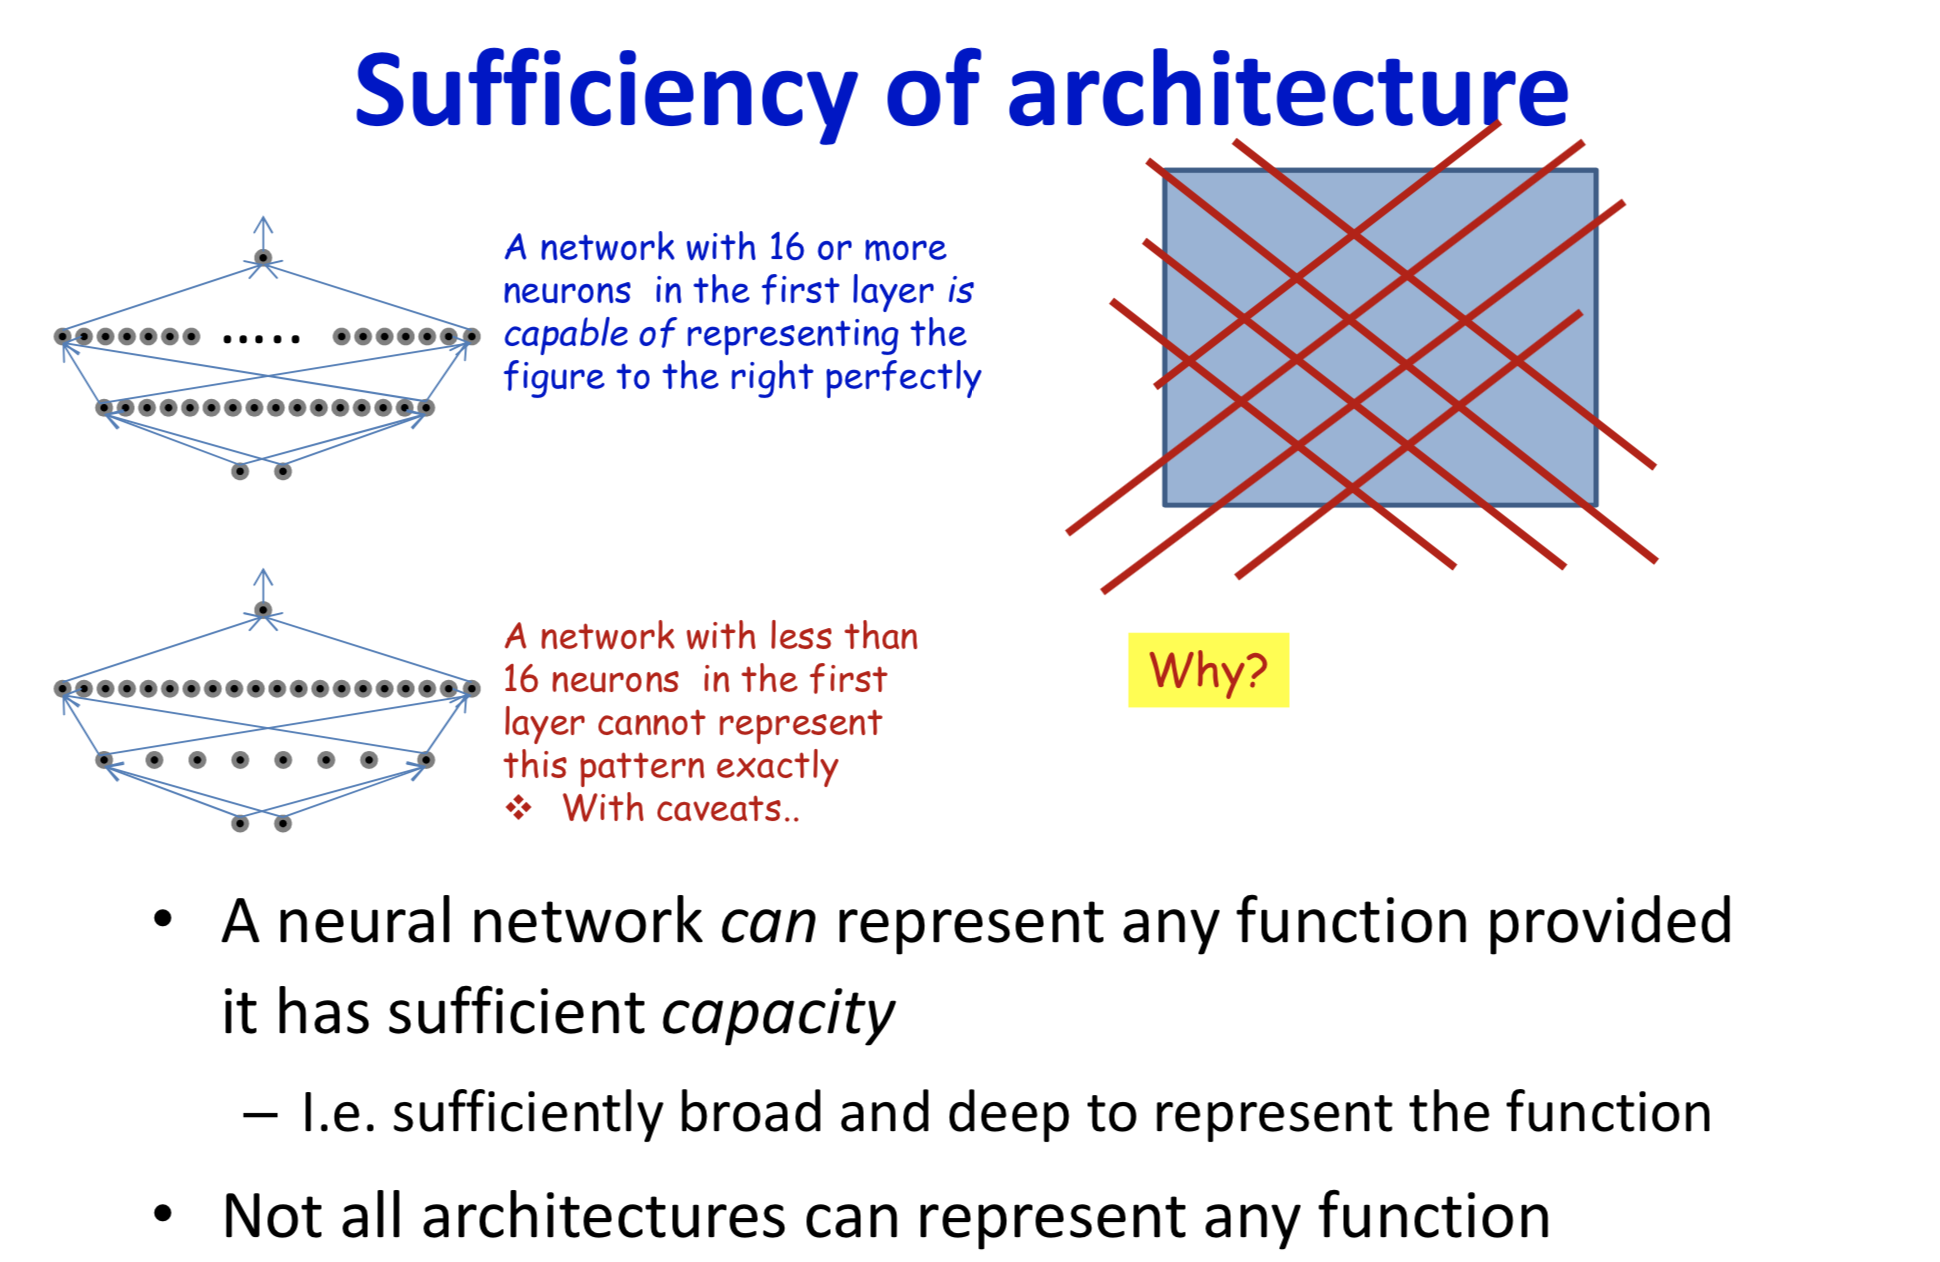
\includegraphics[scale=0.2]{38.png}
	
	Notes: Lost resolution information for squares and strip decision faces
	
	\begin{itemize}
		\item Use other activation functions: sigmoid, tanh, relu, etc.
	\end{itemize}
	
	Compared to the non-black or white of the threshold function, other activation functions provide more resolution information in the capture mode. These resolution information will be passed from the lower layer to the upper layer in the form of a gradient, and even compensate for other information lost by the lower layer.
	
	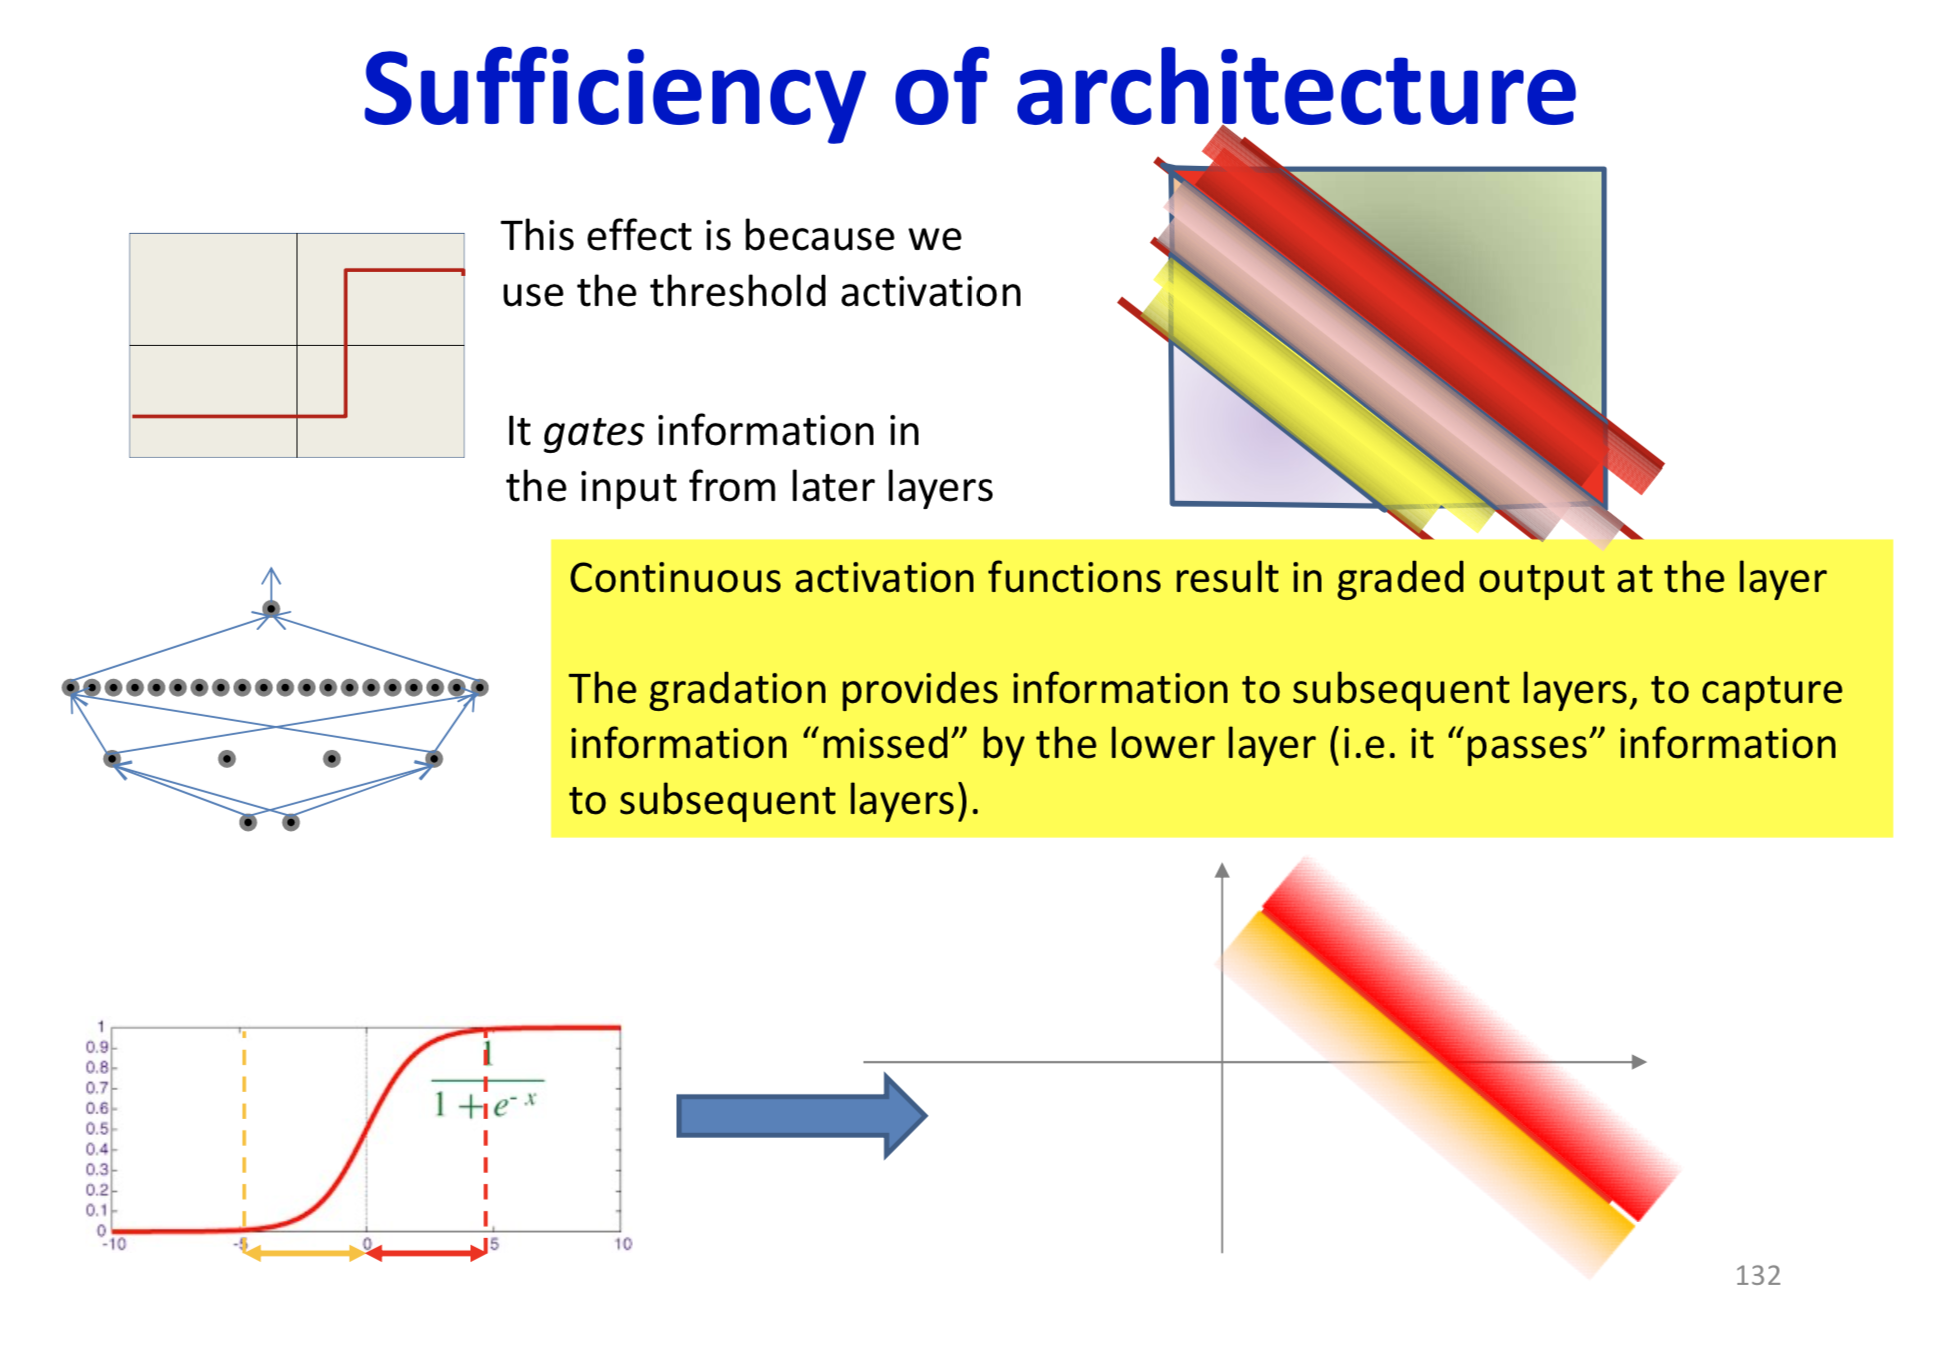
\includegraphics[scale=0.2]{39.png}
	
	Notes: Threshold activation vs sigmoid
	
	The more sufficient the gradient information, the more information can be delivered. For example, relu is better than a more saturated sigmoid. But it also requires a deeper network layer.
	
	A good activation function requires the ability to continuously capture information (relu > tanh > sigmoid), as well as the ability to capture boundaries (relu > linear activation). Therefore, a valid activation function usually requires a turning point and cannot be a purely linear activation.
	
	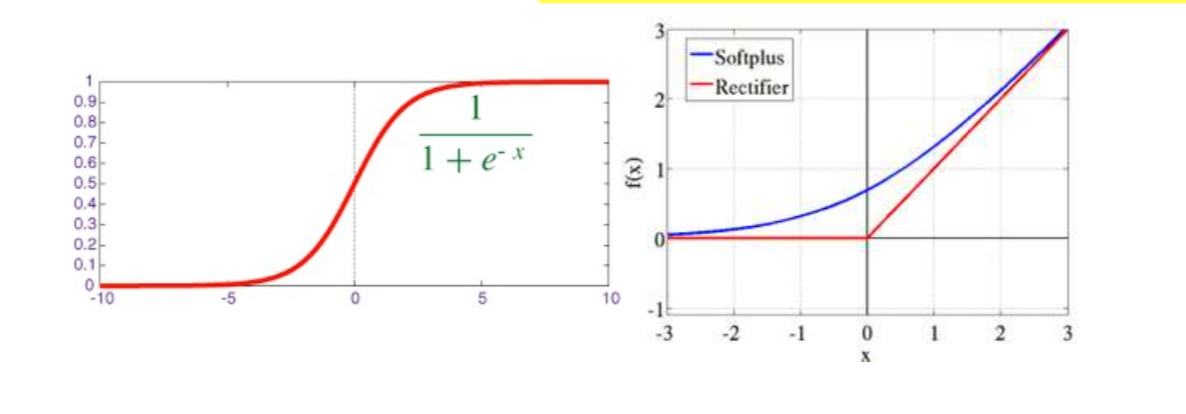
\includegraphics[scale=0.2]{40.png}
	
	Notes: sigmoid vs relu \\ \\
	
	
	\begin{itemize}
		\item Width, depth and activation function trade-offs
	\end{itemize}
	
	In theory, any activation function, even a threshold function, captures all pattern information as long as there is sufficient depth and width.
	
	If threshold activation is used, once the depth and width are not enough, the lost pattern will not be compensated. However, the choice of activation function can alleviate the problem. Choose a good activation function whose gradient will compensate the higher level information lost due to insufficient low-level capacity.
	
	The more you continue to capture the activation function of the mode, the more you will be able to compensate for the missing information. Therefore, this is why people generally use relu to replace sigmoid and threshold functions, because it can capture more information at the same width and depth.
	
	
	
	
	\section{Neural Networks: Part 1}
	
	\subsection{Basic Concepts And Theoretical Foundations}
	
	It mainly introduces the basic concepts and theoretical foundations of training neural networks, including perceptron network training rules and empirical risk minimization theory.
	
	\textbf{1. Preliminaries: The units in the network}
	
	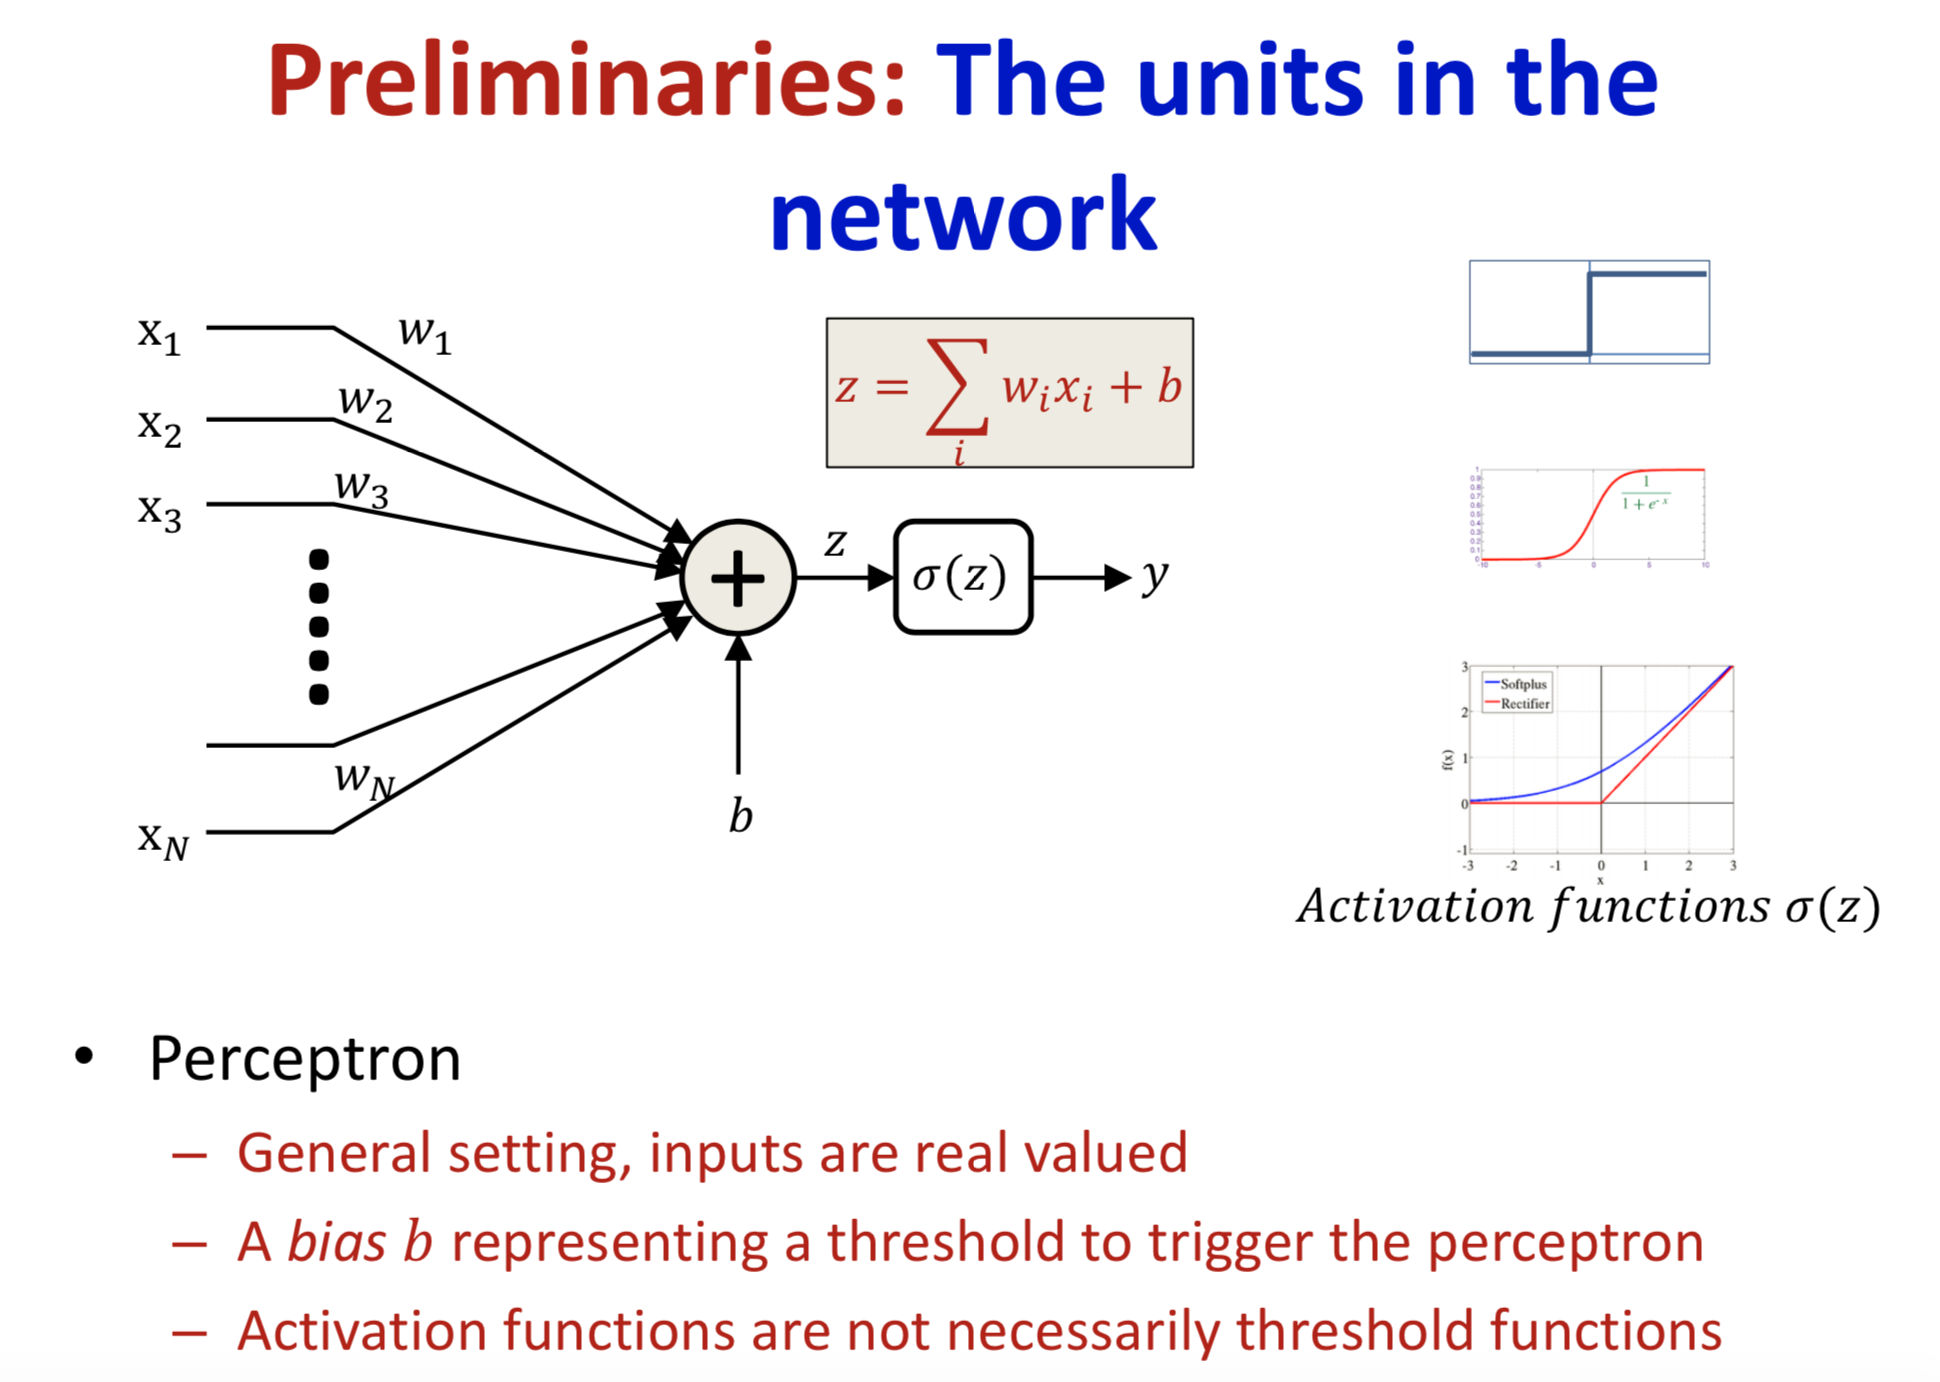
\includegraphics[scale=0.2]{41.png}
	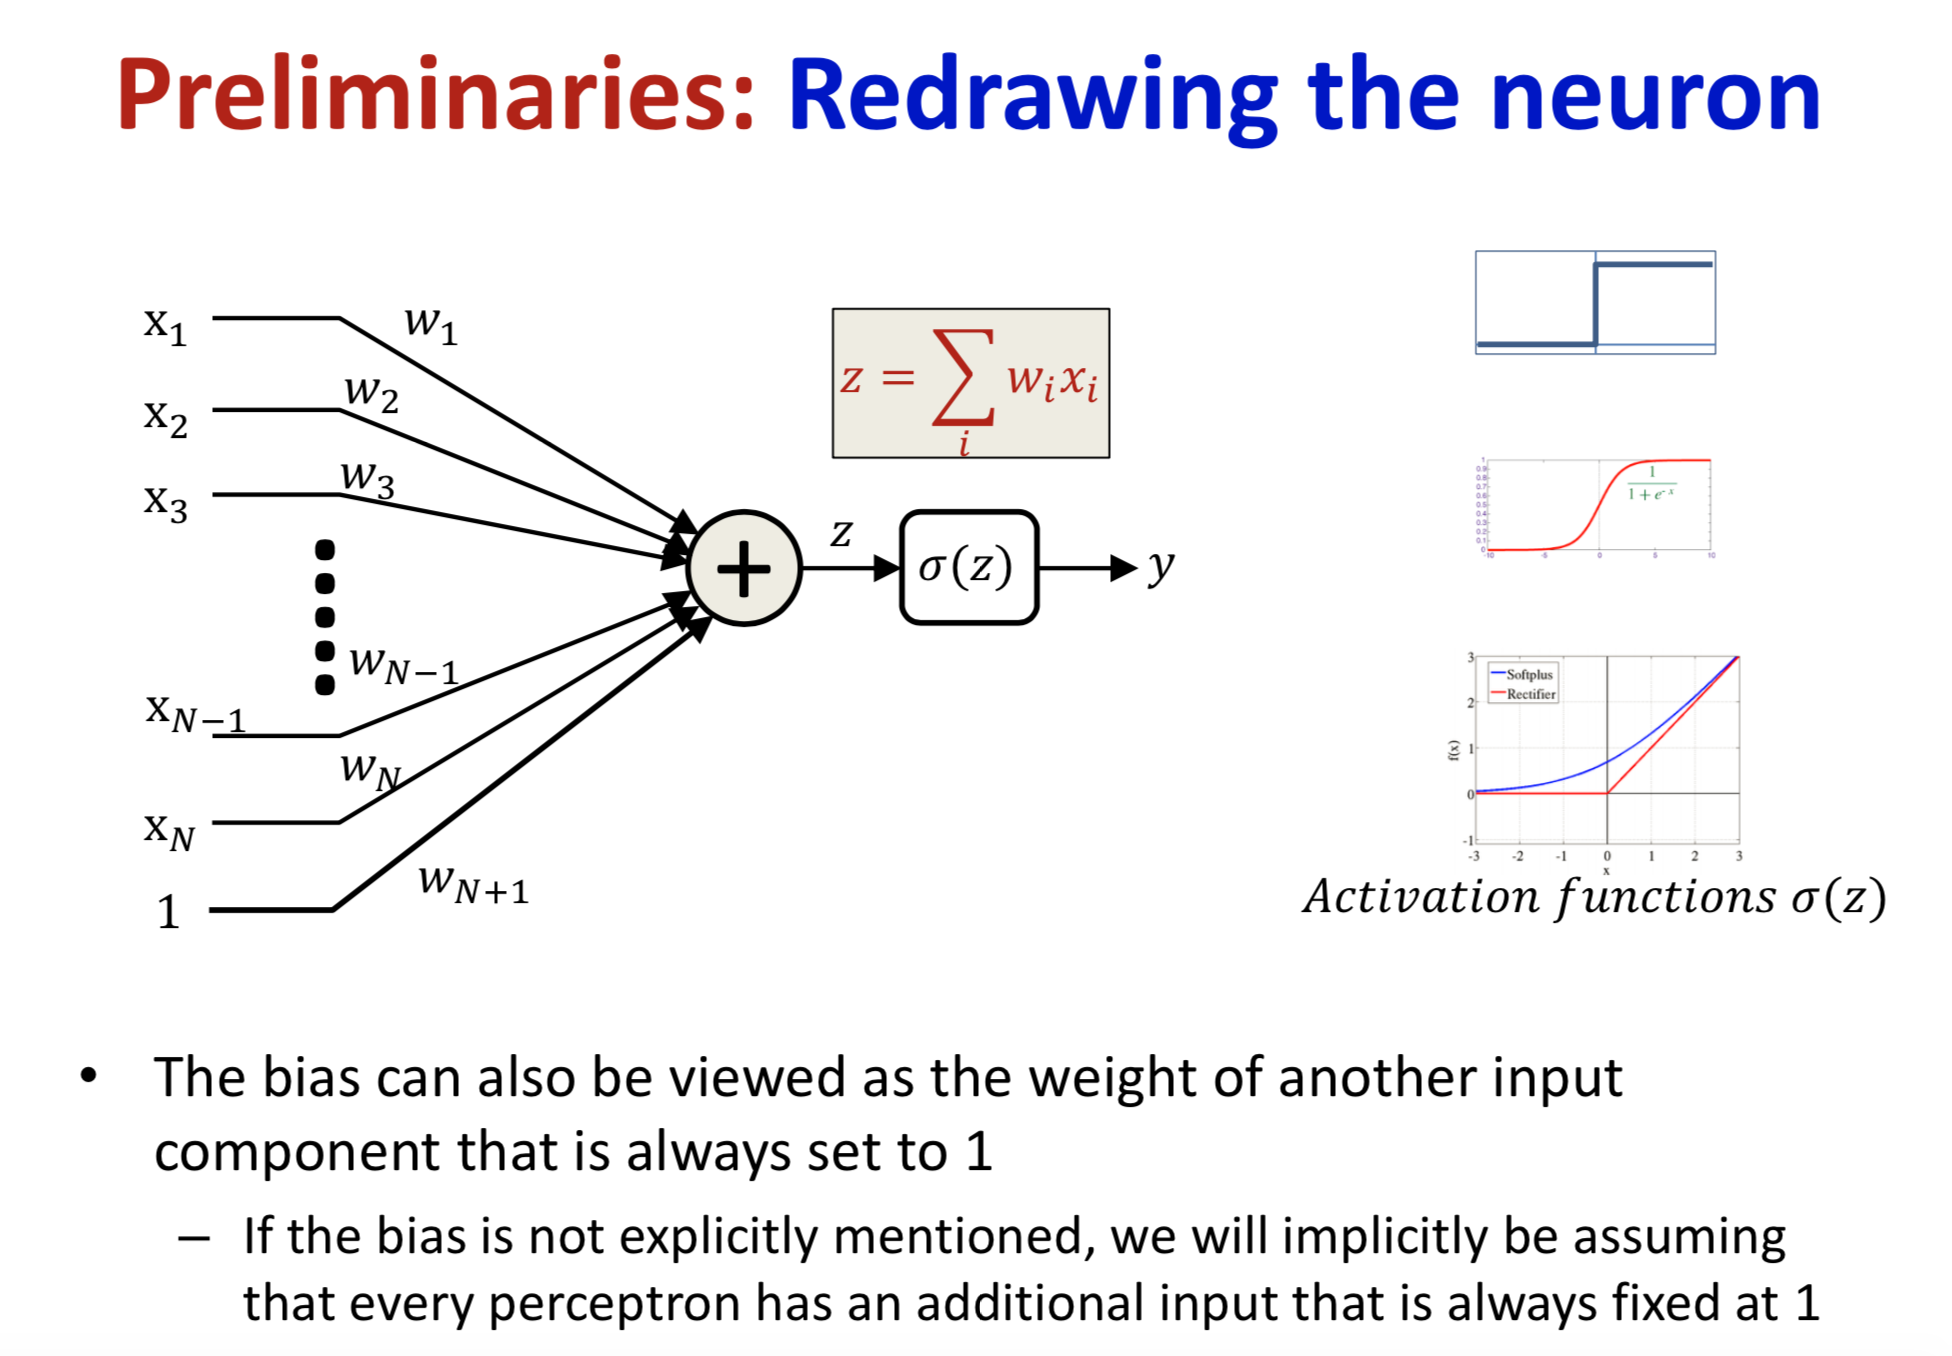
\includegraphics[scale=0.2]{42.png} \\ \\
	
	\textbf{2. Training network: known network structure, fitting function g(X)}
	
	\begin{itemize}
		\item Definition
	\end{itemize}
	
	Assume the network, 
	
	(1) feedforward network (the network is loop-free, the output does not affect the input)
	
	(2) has the ability to fit all functions
	
	Therefore, the training network, that is, under the given network structure, learns the weight parameters of the network.
	
	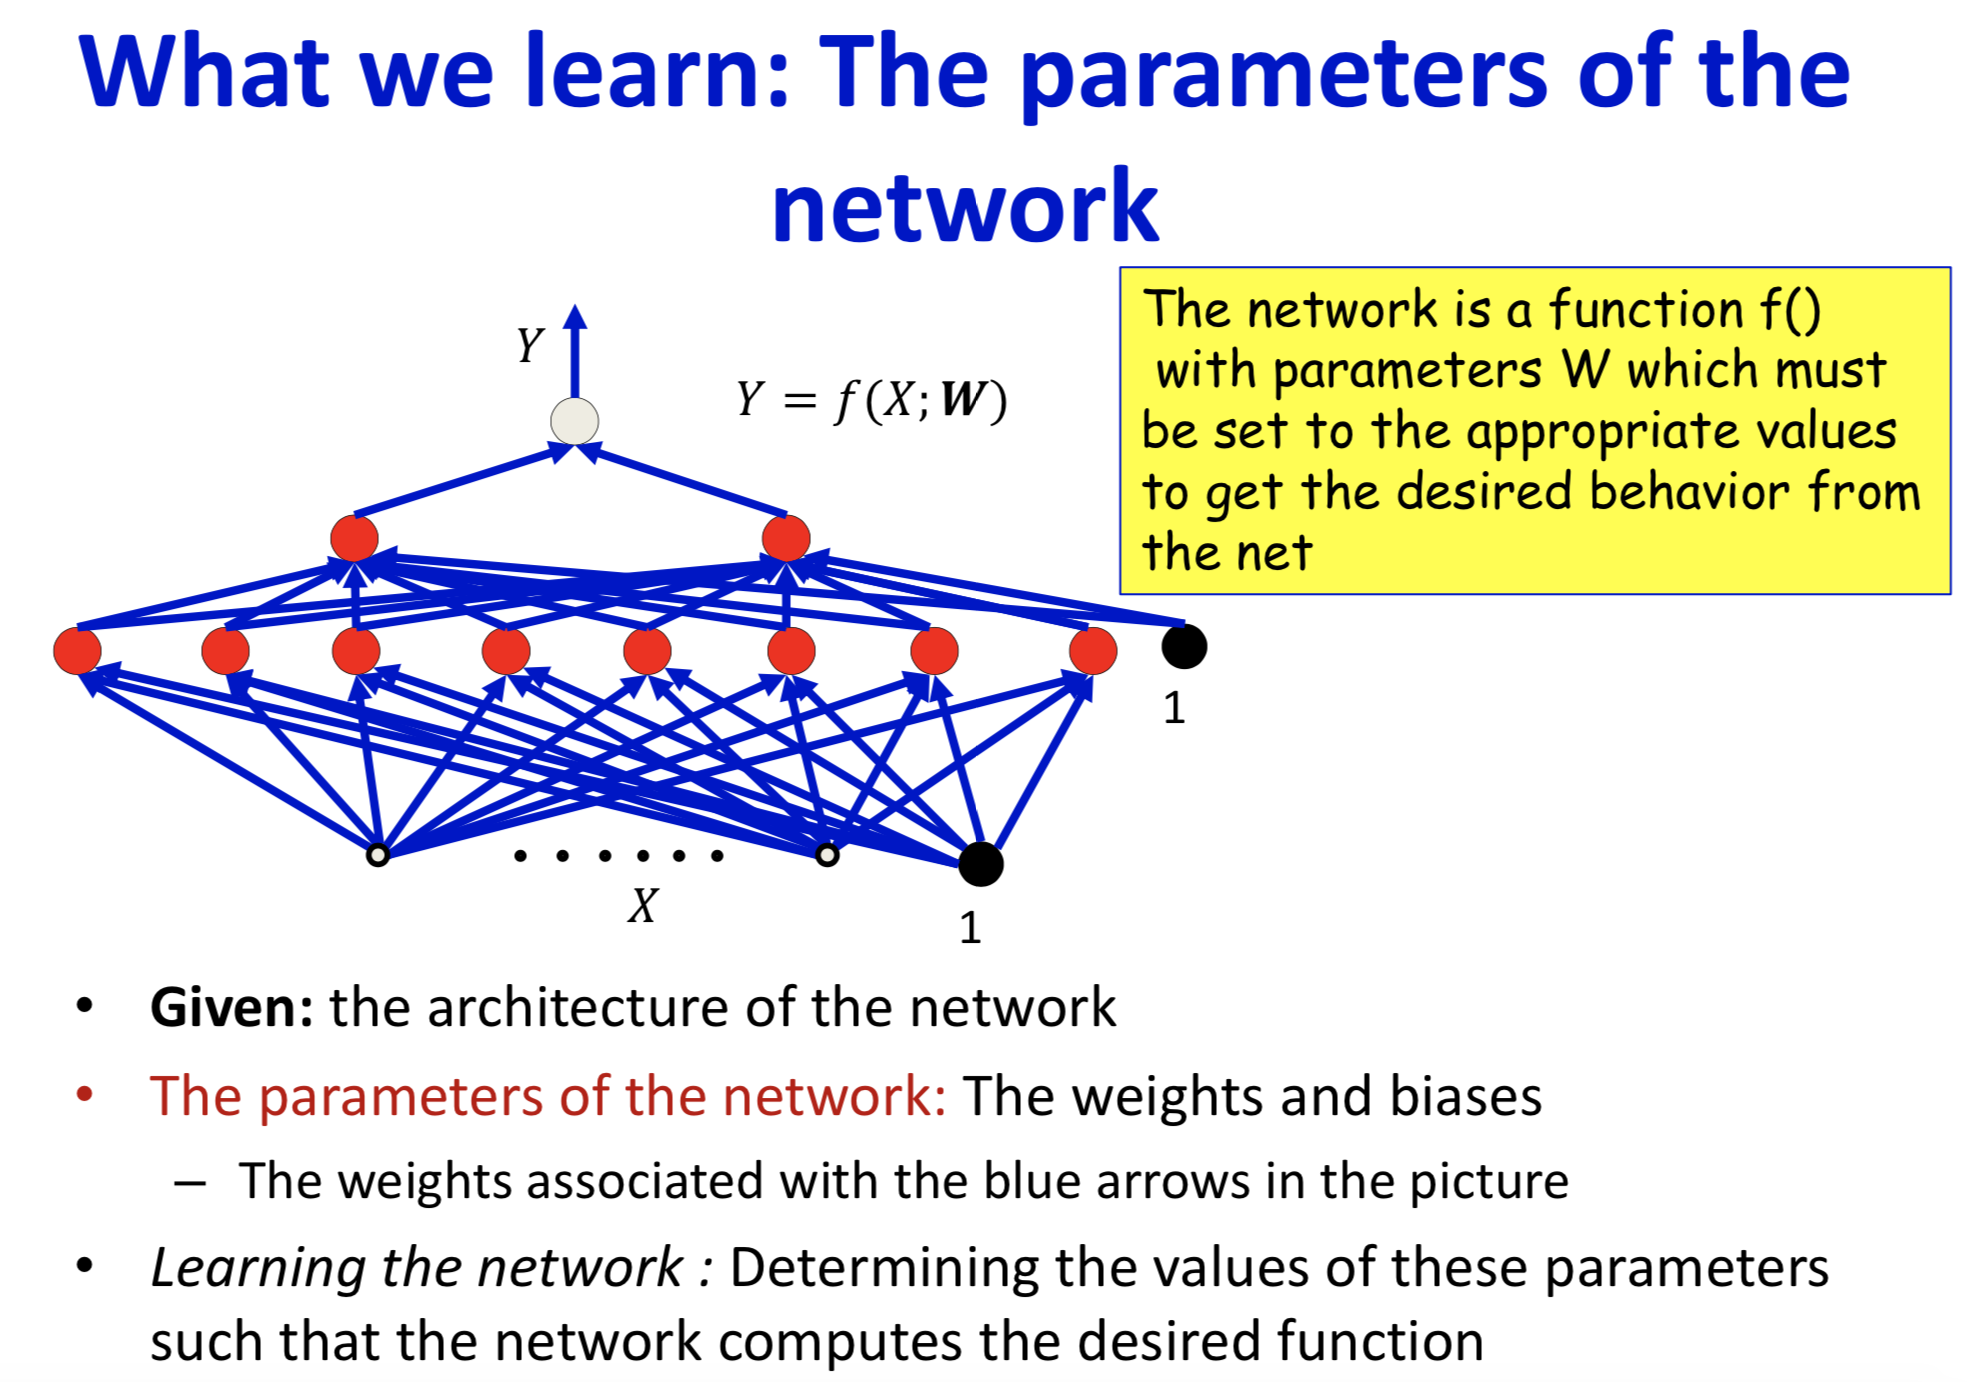
\includegraphics[scale=0.2]{43.png}
	
	Notes: The blue arrow represents the parameter, and the training network determines the value of the parameter to completely fit the function.
	
	
	\begin{itemize}
		\item Objective
	\end{itemize}
	
	Assume that the objective function = $g(X)$, the function of the multi-layer perceptron network training = $f(X;W)$. Therefore, the ultimate goal of training is to minimize the difference between $g(X)$ and $f(X;W)$. In the two-dimensional plane, the training network parameter $W$, the area enclosed by the function curves of $g(X)$ and $f(X;W)$ is minimized. 
	
	The formula is expressed as follows:
	
	$$\hat{W}=\underset{W}{argmin}\int_{x}^{\infty }div(f(X;W),g(X))dx$$
	
	Notes: $div()$ represents the divergence (gap) between functions; the area enclosed by product dispersion.
	
	
	\begin{itemize}
		\item Problem
	\end{itemize}
	
	But in practice, $g(X)$ is unknown. Mathematically, $g(X)$ is estimated by sampling statistics. Therefore, collecting training samples (input->output pairs) is the process of sampling. This is also why the quality of training samples (coverage, uniformity, etc.) will directly affect the accuracy of network training.
	
	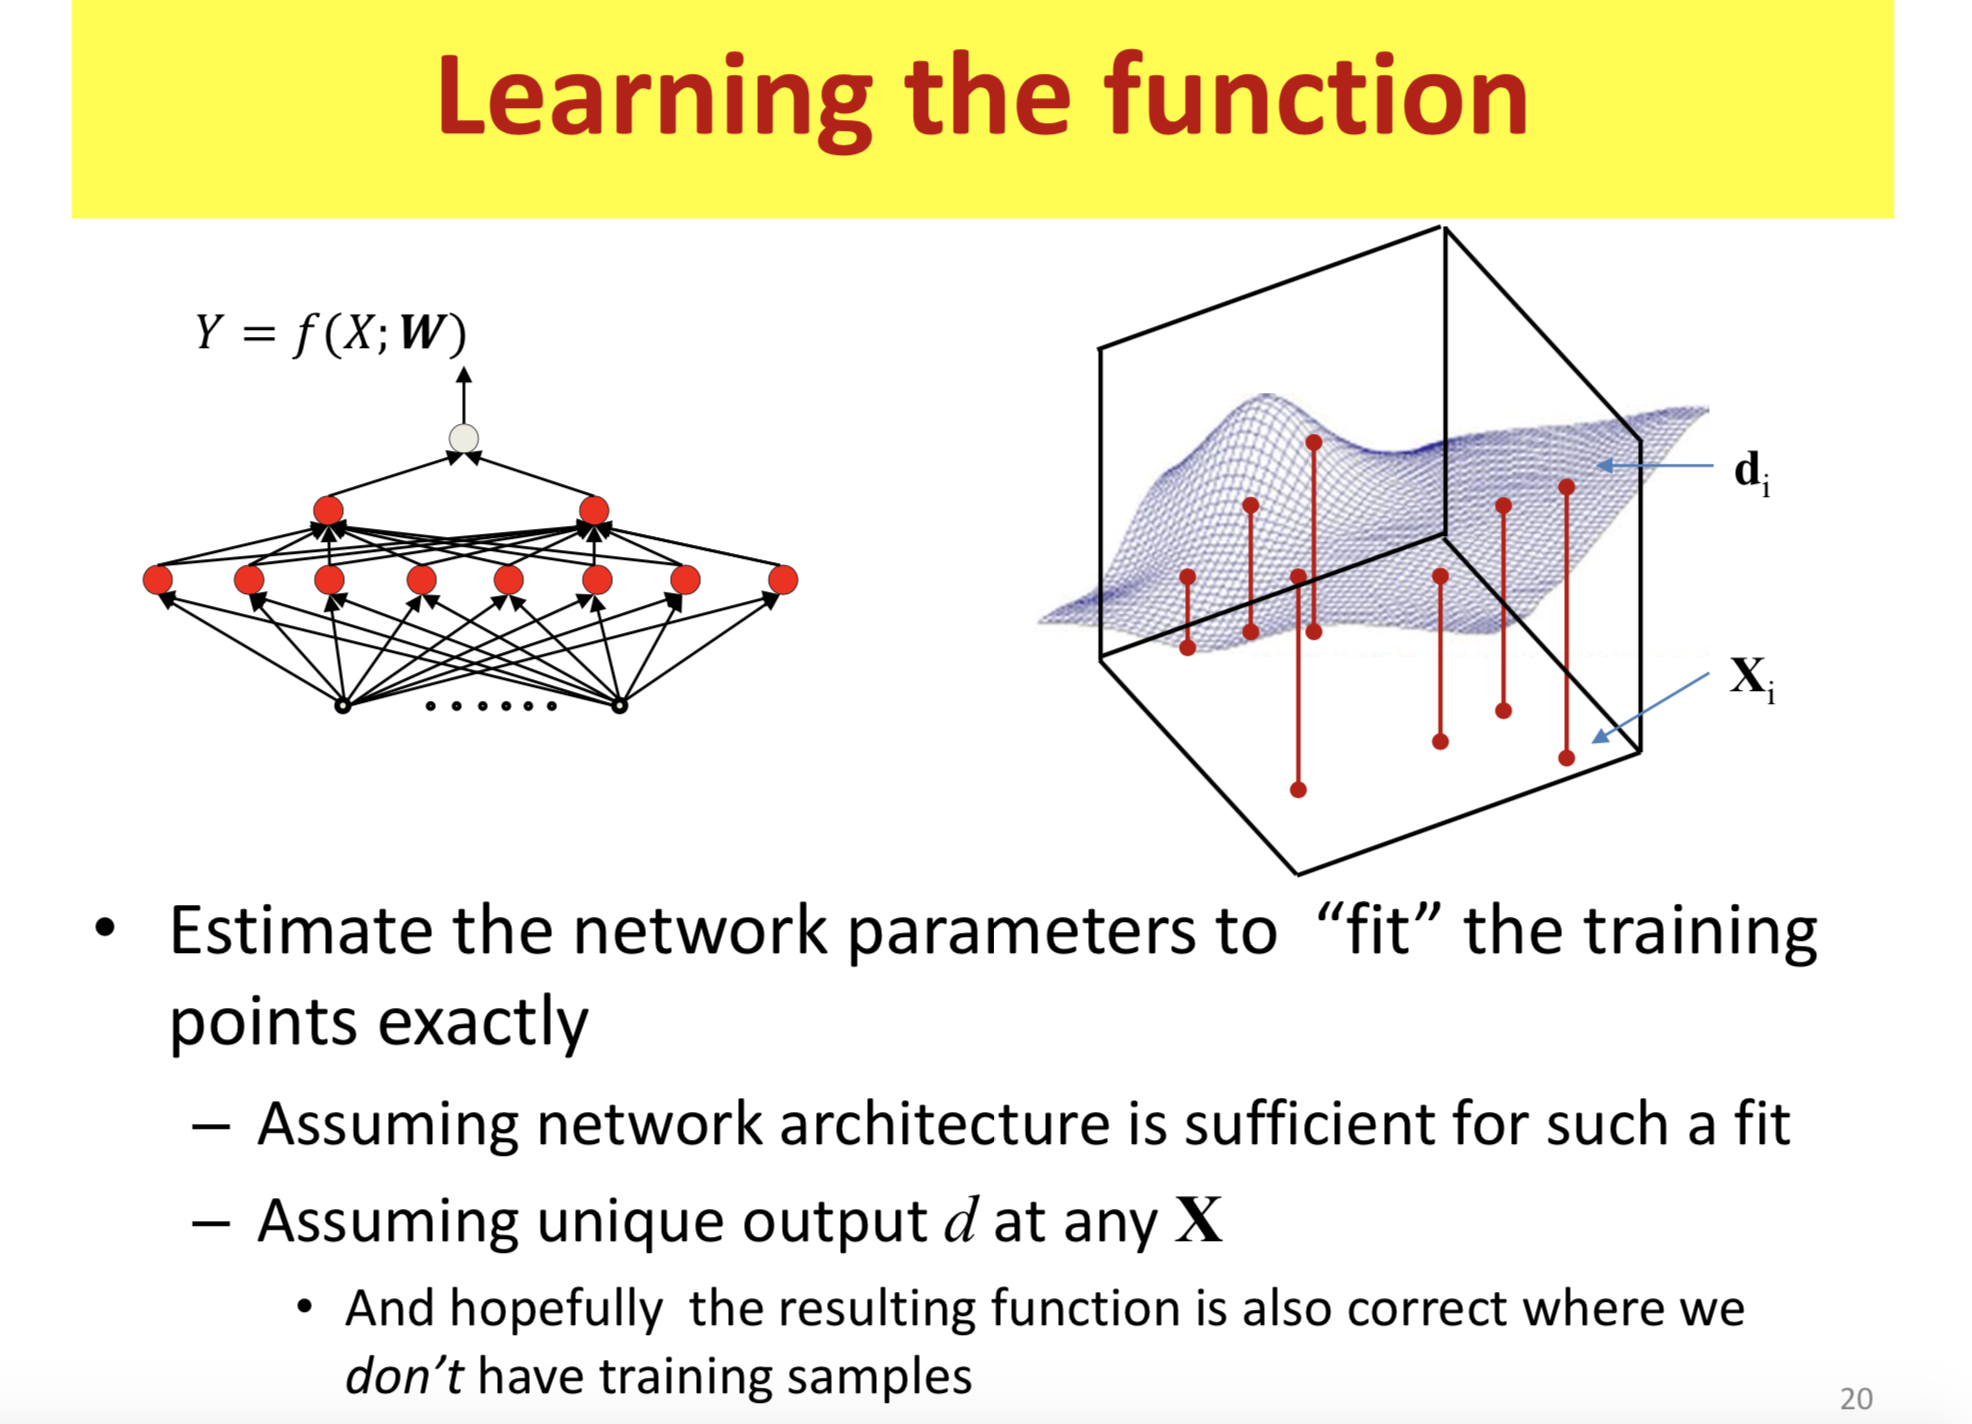
\includegraphics[scale=0.2]{44.png}
	
	Notes: Perceptron network estimates $g(X)$ by accurately fitting the training samples. \\ \\
	
	
	\textbf{3. Start training: taking the two-class problem of a single neuron as an example}
	
	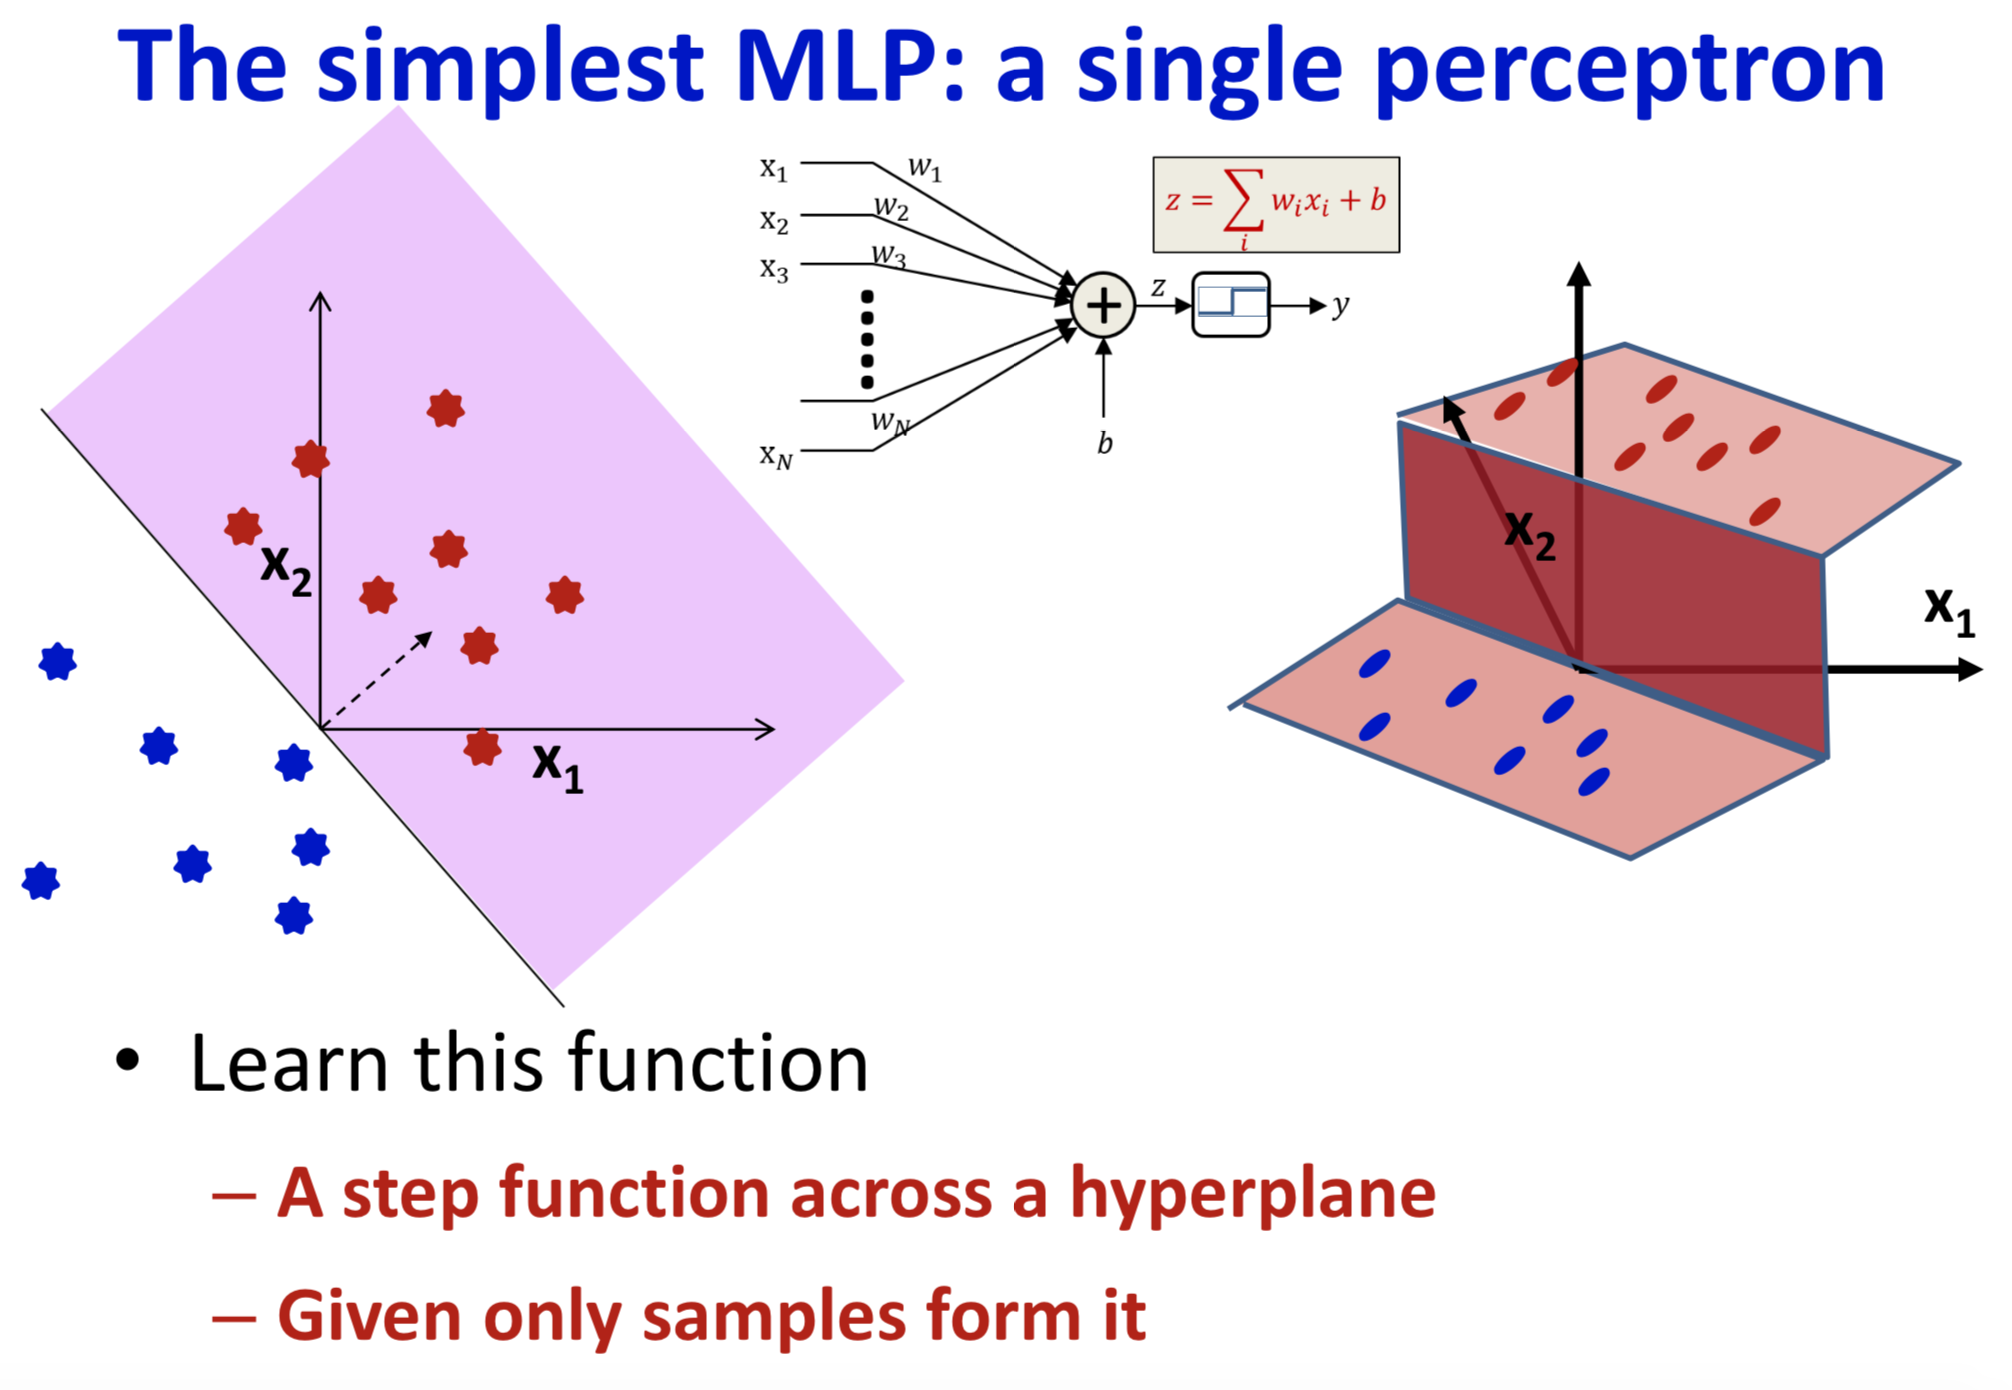
\includegraphics[scale=0.2]{45.png}
	
	
	\begin{itemize}
		\item Algorithm
	\end{itemize}
	
	Find a hyperplane $\sum_{1}^{N+1}{w_i \cdot  X_i}=0$ so that the right and left sides of the hyperplane are separated from the positive and negative classes respectively. From the mathematical expression, it can be regarded as the weight vector $W$ and The inner product between the feature vectors $X$. Therefore, the inner product is 0, that is, the weight vector $W$ and all points on the hyperplane (feature vector $X$) are orthogonal.
	
	\begin{itemize}
		\item Procedure
	\end{itemize}
	
	If the current hyperplane has a wrong class, adjust the hyperplane. The adjustment is done by changing the normal vector $W$ such that if the positive case is misclassified, $W$ is brought closer to the positive case that is misclassified, ie $W'=W+X_i$; if the negative case is misclassified, $W$ is further away from being A negative example of misclassification, ie $W'=W-X_i$.
	
	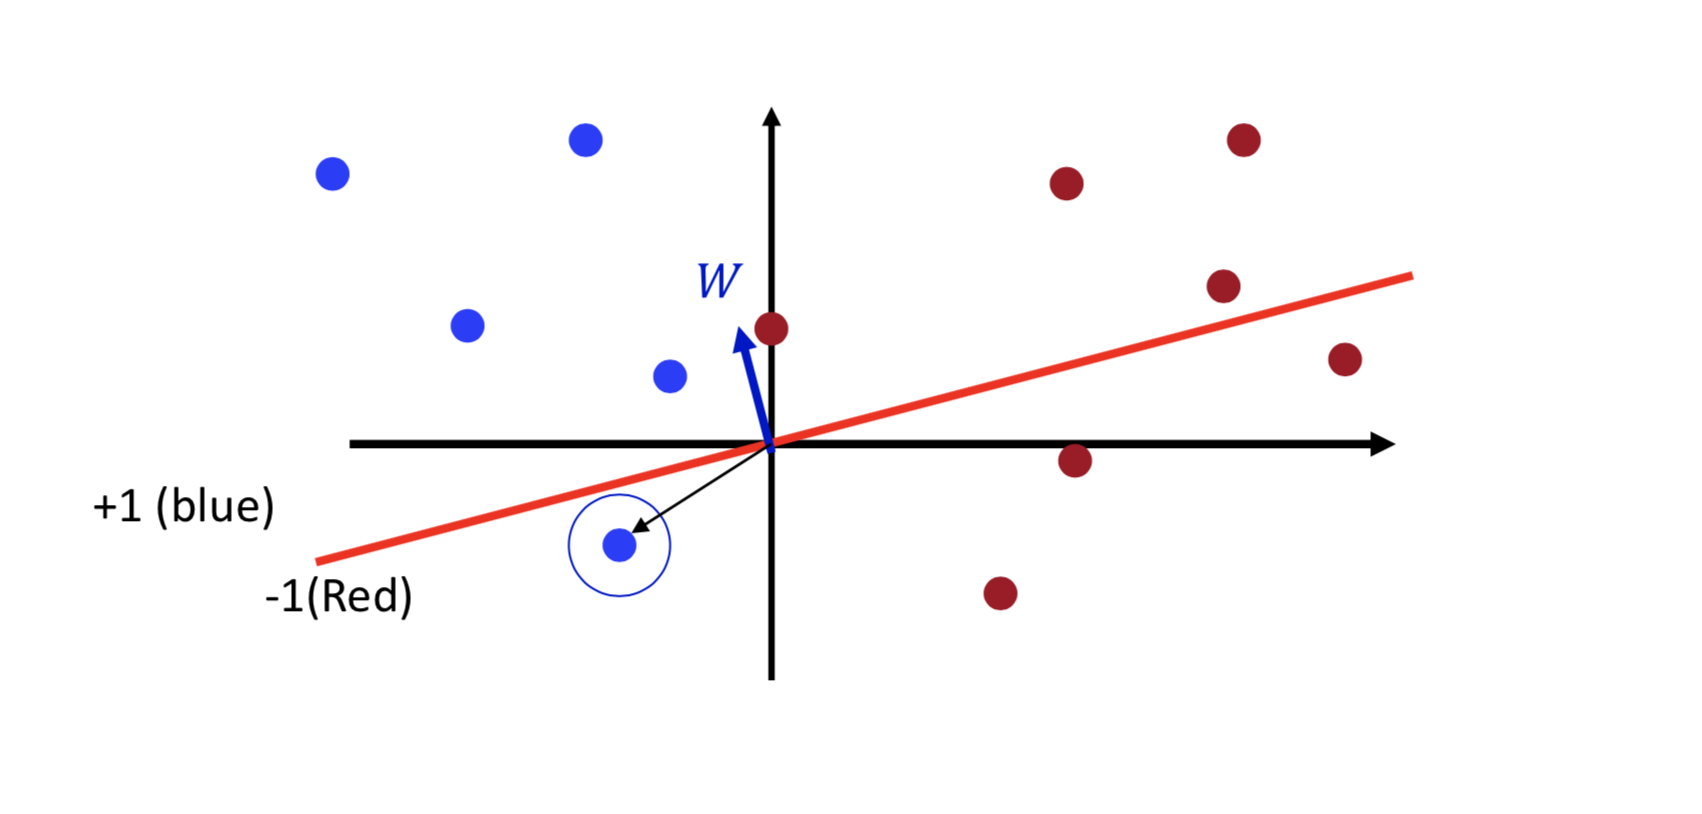
\includegraphics[scale=0.2]{46.png}
	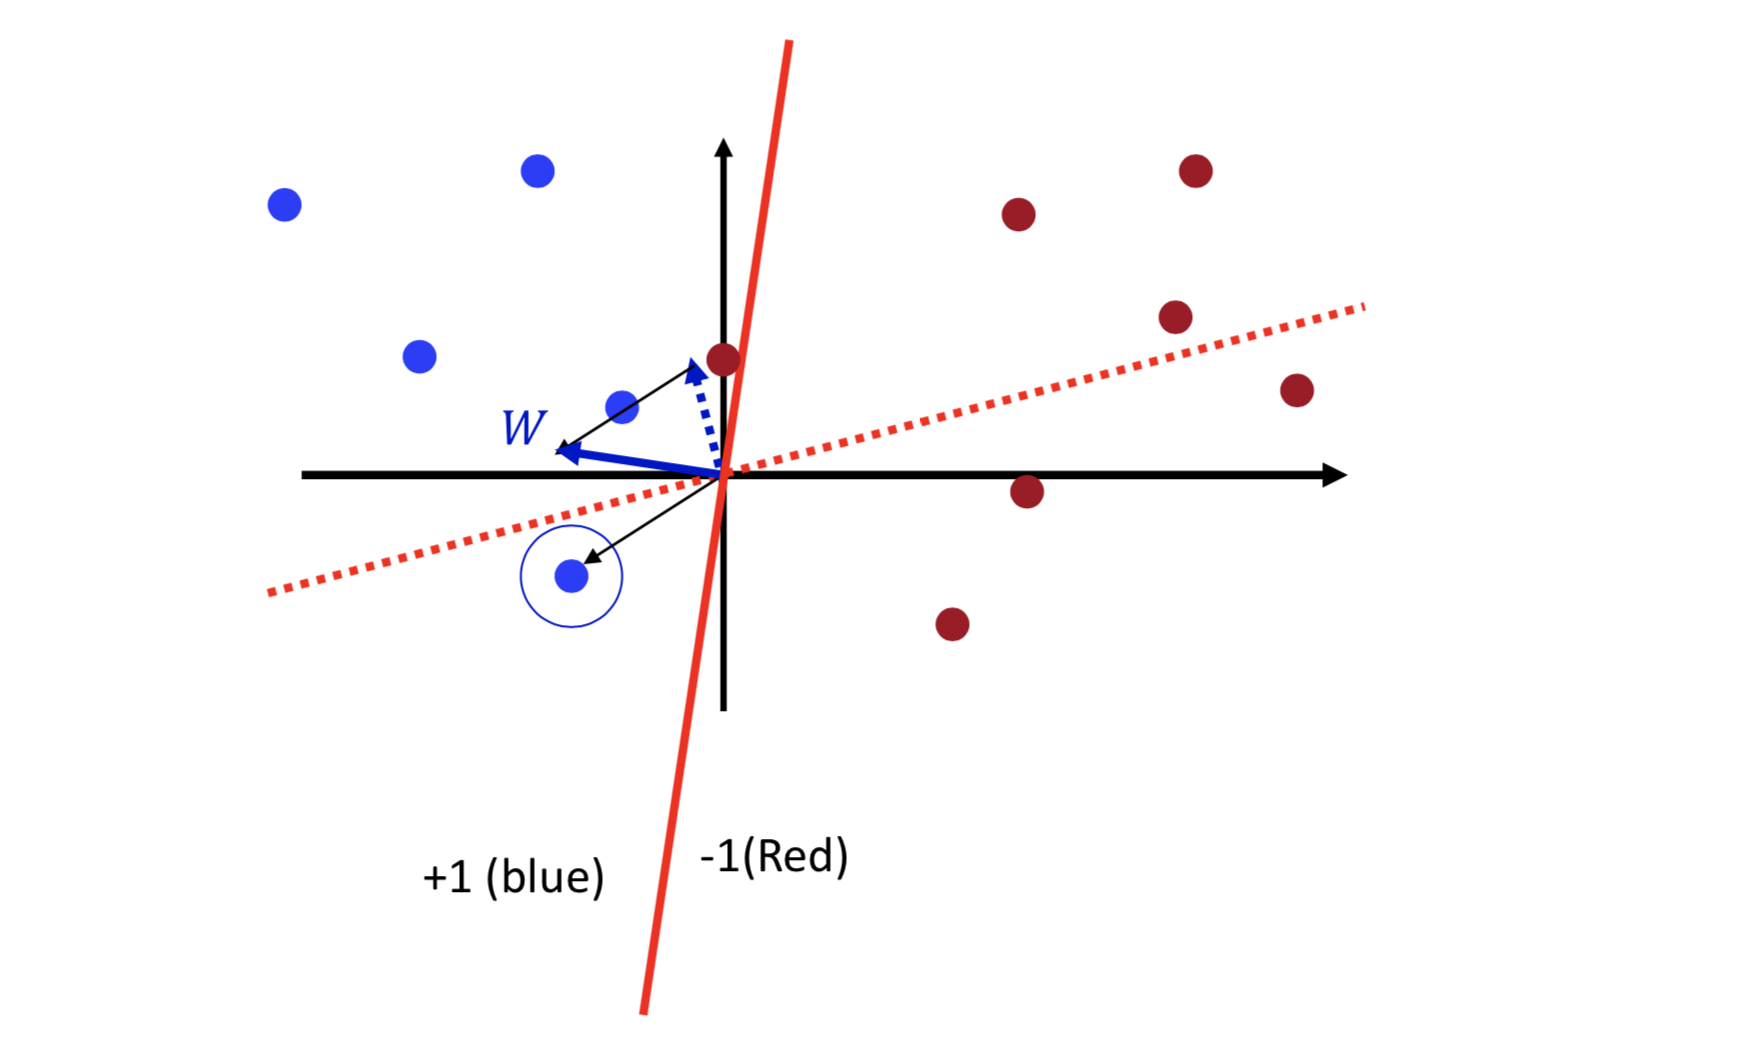
\includegraphics[scale=0.2]{47.png}
	
	Notes: The positive example is misclassified, so that W is close to the positive case of being misclassified.
	
	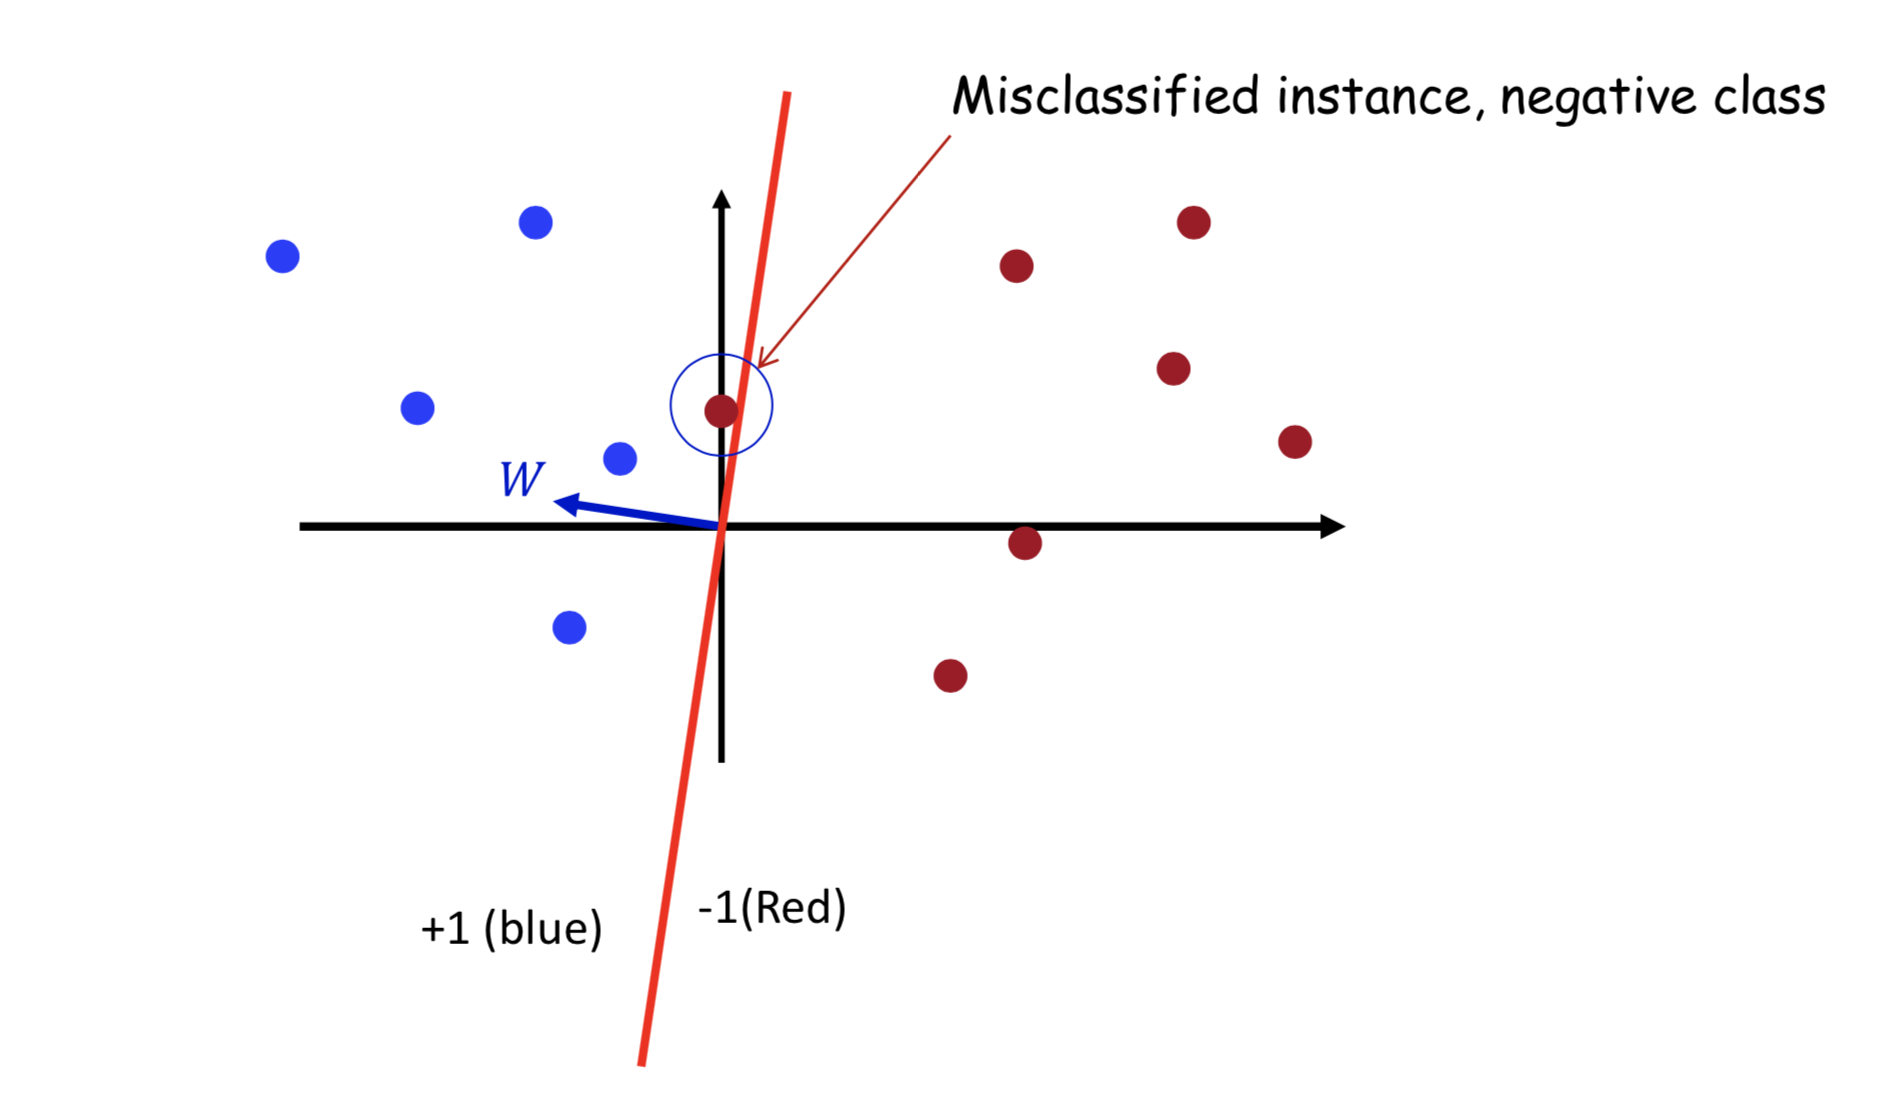
\includegraphics[scale=0.2]{48.png}
	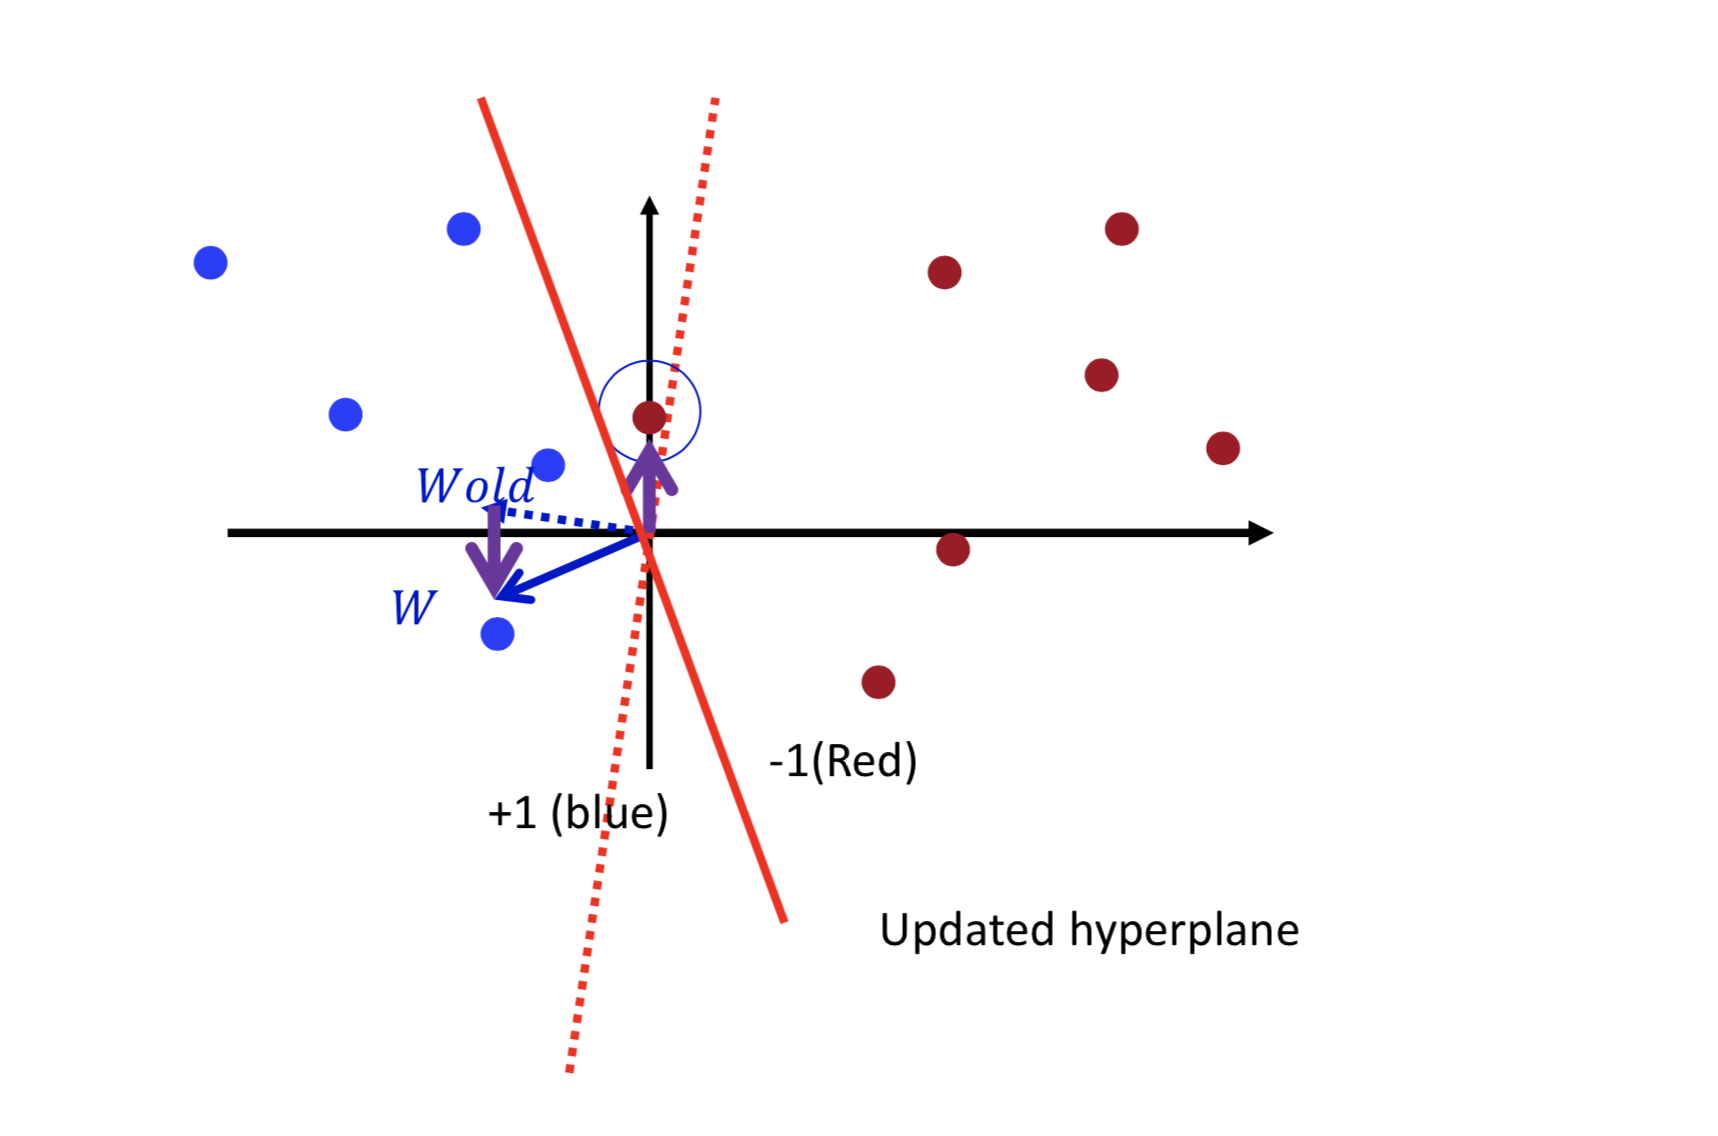
\includegraphics[scale=0.2]{49.png}
	
	Notes: The negative case is misclassified, keeping W away from the negative case of being misclassified.
	
	
	\begin{itemize}
		\item Theory
	\end{itemize}
	
	 What should I do? The theory proves that if the training sample itself is linearly separable, the algorithm must converge, and the number of bad cases does not exceed $(\frac{R}{\gamma})^2$.
	
	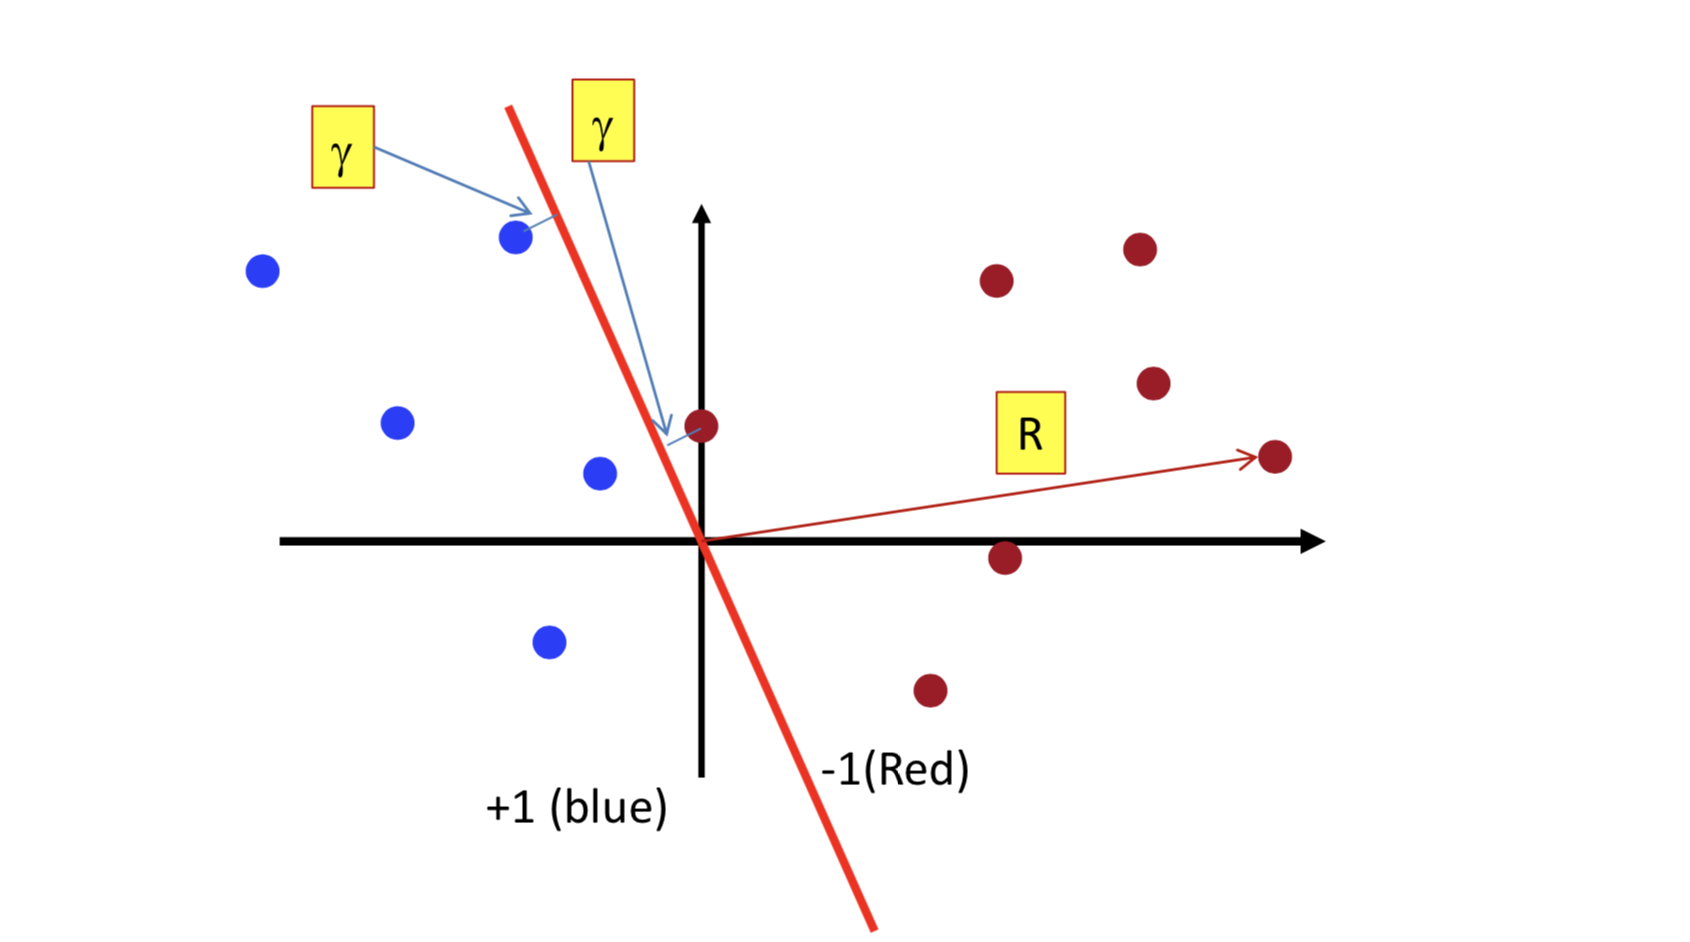
\includegraphics[scale=0.2]{50.png}
	
	Notes: $R$: the length of the farthest sample point. $r$: the closest distance of the correct sample to the classifier. \\ \\
	
	\textbf{4. Advanced training: taking a more complex perceptron network as an example}
	
	\begin{itemize}
		\item Premise
	\end{itemize}
	
	Given training data, perceptron training rules and adequate network structure, how to train a complex network structure, how difficult is the training process? (Training: Get all the parameters in the network)
	
	\includegraphics[scale=0.2]{51.png}
	
	Notes: Positive class: red dot, negative class: blue dot (2 variables, 10 decision lines, 2 pentagons for summation).
	
	\begin{itemize}
		\item Thought
	\end{itemize}
	
	Each decision line is a two-class linear classifier of a single perceptron, but needs to change the label of some samples.
	
	\includegraphics[scale=0.2]{52.png}
	
	Notes: Turn the blue sample on the right side of the decision line into red and start training.
	
	\begin{itemize}
		\item Question
	\end{itemize}
	
	How do I change the label? This also requires training!
	
	In theory, for each decision line, you need to try each method of changing the blue point to red, get different decision faces, and finally choose a correct one. Therefore, in the process of training, it is also necessary to train at the same time, how to modify the rules of the label color for each decision line.
	
	Computationally, this is an exponential search operation, NP problem, it is impossible to obtain the optimal solution on the calculation. But there are 2 greedy algorithms that can try to get suboptimal solutions, namely Adaline and Madaline.
	
	\includegraphics[scale=0.2]{53.png}
	
	Notes: Each neuron must be trained to output all samples, including the output of the modified sample. \\ \\
	
	\textbf{5. Another way of thinking: Why is it so difficult to train the network according to the perceptron rules above?}
	
	\begin{itemize}
		\item Reason
	\end{itemize}
	
	For the threshold function, on any x, non-zero or 1 y, the small change of the weight w will not be immediately fed back to the network, and only if w has changed enough, we know w Whether the change really optimizes the fitting result. That is, the threshold function is a step function, which is the problem!
	
	\includegraphics[scale=0.2]{54.png}
	
	Notes: Step function, unable to act on linearly inseparable training samples.
	
	\begin{itemize}
		\item Optimization
	\end{itemize}
	
	Change the activation function so that the neurons are guided everywhere. That is, any small change in weight w is immediately fed back to the output in a smooth manner.
	
	For linearly inseparable sample points, taking a one-dimensional variable as an example, a suitable threshold function cannot be found to separate the sample points of the lower graph y=0 and y=1. But P(Y=1|X) has a natural probability explanation for this.
	
	\includegraphics[scale=0.2]{55.png}
	
	Notes: Each blue point represents the probability value of y=1 on the corresponding x, ie P(Y=1|X).
	
	For multivariate variables, construct a weighted mean Z between the multivariate variables, and find that P(Y=1|Z) satisfies the probability change of the above graph, which is essentially the expression of logistic regression, the famous sigmoid function.
	
	The chain rule of the derivation is also applicable to the sigmoid function, which makes the whole perceptron network can guide all w of any layer, that is, any w change, the perceptron network output will change.
	
	\textbf{6. Minimize the empirical error: When the objective function cannot be perfectly fitted, make the network as close as possible to it}
	
	\begin{itemize}
		\item Principle
	\end{itemize}
	
	
	When the range of the variable x is limited, it is meaningful to discuss the minimum expected error. When x occurs more frequently in certain intervals, more attention needs to be given to the region. Therefore, more accurately, the training network minimizes the expected error weighted for the probability of occurrence of x.
	
	$$\hat{W}=\underset{W}{argmin}\int_{x}^{\infty }div(f(X;W),g(X))P(X)dx 
	=\underset{W}{argmin}E[div(f(X;W),g(X))]$$
	
	
	\begin{itemize}
		\item Concept
	\end{itemize}
	
	
	The expected error (left of red) is the average error for the entire input space, and the empirical error of the expected error (right of red) is the average error for all training samples.
	
	\includegraphics[scale=0.2]{56.png}
	
	Notes: The empirical error (red to the right) is what is faced in actual training: for training samples.
	
	
	\begin{itemize}
		\item Objective
	\end{itemize}
	
	
	Find a set of ws to minimize empirical error and complete the final training of the entire perceptron network (significantly different from the threshold function-based perceptron training rules). \\ \\ \\
	
	
	\subsection{Gradient Descent Theory and Objective Function}
	
	It mainly introduces the definition of gradient descent theory and neural network objective function as a preliminary knowledge of backward propagation. \\ 
	
	\textbf{1. Gradient descent}
	
	\begin{itemize}
		\item Extreme Value
	\end{itemize}

	Usually at the stagnation point, that is, the derivative is 0. At the same time, if and only if the second derivative of the stagnation point is $>0$, it is a minimum value; when the second derivative is $<0$, it is a maximum value.
	
	\includegraphics[scale=0.2]{57.png}
    
	
	\begin{itemize}
		\item Gradient
	\end{itemize}
	
	If a gradient is defined, it is a row vector consisting of each partial derivative, indicating to what extent $\Delta{\bar{X}}$ affects $\Delta{\bar{Y}}$, with $\Delta{\bar{Y}}=Grade·\Delta{\bar{X}}=|Gradient|·|\Delta{\bar{X}}|·cos\theta$ if and only if $\theta=0$, ie gradient $\Delta{\bar{X}}$ When the direction is the same, $\Delta{\bar{Y}}$ is the largest and $Y$ is the fastest. Similarly, if $\theta=180$, the direction is reversed, $Y$ decreases the fastest.
	
	
	\includegraphics[scale=0.2]{58.png}
	
	Notes: The gradient direction is perpendicular to the contour direction.
	
	
	\begin{itemize}
		\item Optimization
	\end{itemize}
	
	Although the extreme points of the function have analytical solutions, because of the complexity of the calculation, iterative methods are usually used to achieve the goal. The core of the iterative method is the gradient descent, so that X always changes along the opposite direction of the gradient (partial guide vector) until Y is no longer reduced.
	
	So, the question is, given a training set, how to use the empirical error minimization theory, define the objective function f(X), and use the gradient minimization to train the neural network model?
	
	
	\textbf{2. Objective function}
	
	\begin{itemize}
		\item The definition of the premise
	\end{itemize}
	
	Because the gradient is to be used, the objective function must be continuous, and each parameter is measurable everywhere. Therefore, the neural network must use the activation function and redefine the error function instead of the number of misclassifications as the objective function.
	
	\begin{itemize}
		\item Activation function
	\end{itemize}

	In theory, any differentiable function can be used as an activation function. But usually, there are four activation functions as follows:
	
	\includegraphics[scale=0.2]{59.png}
	
	Notes: Sigmoid, Tanh, ReLU, Softplus
	
	
	\begin{itemize}
		\item Typical structure and parameter definitions
	\end{itemize}
	
	
	Input layer: neural network layer 0, input is output, no neuron, $y_i^{0} = x_i$.
	
	Output layer: the Nth layer of the neural network, $y_i=y_i^{N}$. Usually a single real or real vector.
	
	Hidden layer: the middle layer of the neural network, containing $w_{ij}$ and $b_j2$ parameters. Where $w_{ij}^{k}$ = the $i$th neuron of the $k-1$th layer points to the weight of the $j$th neuron of the $k$th layer; $b_j^{k}$ = the $j$th neuron of the $k$th layer Offset.
	
	\includegraphics[scale=0.2]{60.png}
	\includegraphics[scale=0.2]{61.png} \\ \\ \\ \\
	
	\begin{itemize}
		\item The input/output layer represents
	\end{itemize}
	
	
	Input layer: usually a real value vector such as a pixel value, a speech feature or an embedded representation of text.
	
	Output layer:
	
	when the output is real (regression), no special treatment is required.
	
	when the output is a binary representation (classification), first use 0/1 (two classification) or one-hot (multi-class) to indicate yes/no or true label, use sigmoid=P(Y =1|X) or Softmax=$P( Y_i =1|X)$ represents the output probability of the neural network.
	
	\includegraphics[scale=0.2]{62.png}
	\includegraphics[scale=0.2]{63.png}
	
	\begin{itemize}
		\item Objective function definition: (Y = neural network output, d = real label)
	\end{itemize}
	
	
	\includegraphics[scale=0.2]{64.png}
	
	Notes: The core of the objective function is to define Div(Y,d).
	
	Real value output (regression): Euclidean distance
	
	$$Div(Y,d)=\frac{1}{2}||Y-d||^2=\frac{1}{2}\sum _i(y_i-d_i)^2$$
	
	Two classification problem: cross entropy
	
	$$Div(Y,d)=-dlogY-(1-d)log(1-Y)$$
	
	Multi-classification problem: cross entropy
	
	$$Div(Y,d)=-\sum _id_ilogy_i$$
	
	\textbf{3. Training algorithm}
	
	\includegraphics[scale=0.2]{65.png}
	
	
	\section{Neural Networks: Part 2}
	
	\subsection{Backward Propagation Theory And Convergence}
	
	It mainly introduces the two parts of the neural network's "backward propagation theory" and "convergence". \\
	
	\textbf{1. Backward propagation, is it effective? That is, can it help the neural network find the global best?}
	
	In the classification problem, because of the discrete output, the classification error function is not a microscopic function in nature. Therefore, in practice, only one softmax layer can be added to the neural network of the classification problem, and then a new one can be added. A micro-objective function (for example, crossover), as a "proxy function", evaluates the classification problem. However, please note that minimizing this "proxy function" may not be the optimal solution to the classification problem. As shown in the figure below, for a perceptron, in the left picture, the backward propagation can find the global best, but in the right picture, an abnormal deviation point is added, and the backward propagation does not track each point. Therefore, only a small reaction to the new point (red) is obtained, and the global optimal solution (blue) cannot be obtained. This is a feature of backward propagation because its “low variance” may lead to better generalization effects.
	
	\includegraphics[scale=0.2]{66.png}
	\includegraphics[scale=0.2]{67.png}
	
	Even in the data with a few abnormal points, the neural network constructed by the multi-layer perceptron can not find the global optimal solution. This is mainly because the answer to the optimal separation is not the optimal solution that the "agent function" can achieve. There are many authoritative research papers that discuss the neural network error surfaces with a large number of saddle points.
	
	\includegraphics[scale=0.2]{68.png}
	\includegraphics[scale=0.2]{69.png}
	
	
	\textbf{2. Backward propagation, can it converge, and how fast does it converge?}
	
	First, we simplify the problem by using the gradient descent method to solve a univariate quadratic objective function with a global minimum, the starting position of the $w^{(k)}$ iteration:
	
	\includegraphics[scale=0.2]{70.png}
	
	How to choose the learning rate of gradient drop $\eta$ ? The best solution, I hope to achieve the best in one step. Because the objective function is so simple, the $w_{min}$ at the minimum can be obtained directly by Newton's method, so the optimal learning rate $\eta_{opt}$ is also in the limelight.
	
	\includegraphics[scale=0.2]{71.png}
	
	When $\eta$ is not the optimal learning rate, the iteration of the gradient descent is shown in the figure below. 
	
	Note the choice of $\eta$ when converging, oscillating, and diverging.
	
	\includegraphics[scale=0.2]{72.png}
	
	Next, we discuss a more general case, using the gradient descent method to solve a multi-objective quadratic objective function with global minimum: the function value E is a scalar with $E^T=E$, so A must be a symmetric positive definite matrix. All eigenvalues are also positive numbers. Furthermore, assuming that A is a diagonal matrix consisting of eigenvalues, the objective function can be simplified such that the arbitrary variables $w_i$ are decoupled from each other and parallel to the function space axis. At the same time, under the premise of ensuring that other variables are unchanged, arbitrarily select two variables ($w_1$, $w_2$) and function value E to form an elliptical contour, and select one of the variables ($w_1$, $w_2$) and the function value respectively. E, projected to the plane. Therefore, the function expression and optimal learning rate $\eta_{opt}$ in the two cases, as shown in the figure, at this time, $\eta_{opt}<2*min(\eta_{i,opt})$ is the optimal choice.
	
	\includegraphics[scale=0.2]{73.png}
	\includegraphics[scale=0.2]{74.png}
	\includegraphics[scale=0.2]{75.png}
	
	However, in a function, $\eta_{i,opt}$ in different directions is varied and the gap is very large, so the learning rate selected according to the above principle usually converges very slowly. Therefore, scaling the target function axis, normalizing the objective function, making $\eta_{i,opt}$ equal in all directions, will make it easier to find an optimal learning rate.
	
	\includegraphics[scale=0.2]{76.png}
	
	Eventually, along a diagonal matrix, the axis is scaled and the contours are changed from ellipse to circular. According to the previous assumption, the matrix A itself is a diagonal matrix composed of one eigenvalue, and therefore, the new transformation matrix S will be the square root of the matrix A. At this time, the comprehensive optimal learning rate is equal to one.
	
	\includegraphics[scale=0.2]{77.png}
	
	For the more general matrix A, the variable $w_i$ is not completely decoupled. That is, if the matrix A is not a diagonal matrix, the contours will no longer be parallel to the coordinate axes. But after the axis is first "rotated" and then "zoomed", the discussion is still similar.
	
	
	\includegraphics[scale=0.2]{78.png}
	
	But a new problem is that when the second derivative is obtained, a Hessian matrix is added. Therefore, the gradient descent also needs to calculate the inverse matrix of the Hessian matrix.
	
	
	\includegraphics[scale=0.2]{79.png}
	
	Note that this is still not the whole problem. For the ordinary symmetric matrix A, it is very likely to be semi-definite, that is, the eigenvalue may have a negative value and cannot solve its square root. At the same time, even if the matrix A is positive, this is almost impossible to achieve for a neural network with a large number of parameters. Therefore, it is best not to use the Hessian matrix directly. Some optimization algorithms achieve the same goal by approximating the Hessian matrix, such as the BFGS and Levenberg algorithms, but they have recently appeared less because we have better algorithms. It will be introduced in the next lesson.
	
	Finally, the function that the neural network needs to fit is not a convex function. Therefore, a relatively large learning rate may be exactly what it needs, because a large learning rate helps to jump out of the local optimal solution. However, please note that after reaching the search interval of the global optimal solution, the large learning rate will not find the optimal solution. Therefore, in order to balance the relationship between the two, the more common practice is to gradually attenuate the learning rate in the process of training, and there are many ways to achieve it, as shown in the following figure:
	
	\includegraphics[scale=0.2]{80.png}
	\includegraphics[scale=0.2]{81.png} \\ \\ \\
	
	
	\section{Neural Network Training}
	
	It mainly introduces the most important four parts of neural network training: three methods of gradient descent (Batch, Stochastic, mini-Batch), and several methods of optimization algorithm (Momentum, Nestorov, Adagrad, ADAM, RMS Prop, AdaDelta), Generalization strategy (L2 regularization, Dropout) and neural network training techniques (difference evaluation function, Batch Normalization, gradient cutting, data expansion).
	
	
	\subsection{Concept combing}
	
	\begin{itemize}
		\item In traditional data mining tasks, use traditional machine learning
	\end{itemize}
	
	Assuming that the form of the function/model H(x) is given, the purpose of learning is to find several features as the independent variable $x_i$ of H(x), and select different parameters under the criterion of minimizing divergence. The estimation method, while defining the loss function J(x), iteratively updates the parameter $w_i$ of H(x) such that the divergence of J(x) on the training set is minimal. The method of iteratively updating parameters usually uses gradient descent or Newton's method.
	
	Taking logistic regression as an example, it uses the linear weighted + sigmoid function as the given model H(x), and explores the different features $x_i$ in the training data by means of feature engineering, based on the premise of minimizing the evaluation criteria of divergence. The maximum likelihood estimate, as J(x), uses gradient descent to iteratively update the model parameter $w_i$ that is most likely to produce this batch of training data.
	
	Therefore, the most important place in the traditional machine learning method is 3 points. 
	
	(1) Find the adaptive hypothesis function H(x) according to the specific scene;
	
	(2) Feature engineering, find the adaptation function in the training data. The independent variable $x_i$;
	
	(3) selects the implementation of the minimum divergence evaluation criterion, that is, the loss function J(x).
	
	\begin{itemize}
		\item In the face of very large training data sets and extremely complex application scenarios, use deep learning 
	\end{itemize}
	
	Combining specific activation functions, constructing different neural networks (CNN, RNN), and using neural networks to fit the conclusions of arbitrary functions, expecting it to automatically adapt to the hypothesis function H(x) to train the data itself ( End-to-end or feature engineering (other scenarios), etc., define the $x_i$ of the model input. Under the criterion of minimizing the divergence, use the method of minimizing the empirical error to define the L2 divergence or KL divergence as the loss function J. (x), using the gradient descent, iteratively updating the network parameter $w_i$ such that the L2 divergence or KL divergence is minimized.
	
	In the gradient of the neural network, because the network level is too much or too deep, the algorithm framework of backward propagation (ie, a dynamic programming idea) is born to speed up the training; because of the huge training data, the memory The effects of limitation and convergence have resulted in gradient descent methods such as SGD and mini-Batch. In each iterative update of parameters, different numbers of training data are used to achieve time, space and effect trade-offs; The non-convex characteristics, the probability that the neural network converges to local optimum or simply diverges, the optimal methods such as Momentum and ADAM are born, and the optimal convergence effect is obtained as much as possible.
	
	\subsection{Three ways to reduce the gradient}
	
	\textbf{1. Batch gradient descent}
	
	Usually the loss function minimizes the divergence of the predicted and actual values on the entire training sample, so every iteration update of the normal gradient drop requires the use of the entire training set data.
	
	Taking the linear regression of L2 divergence as an example:
	
	\includegraphics[scale=0.4]{82.png}
	
	Take the visual understanding of the image as an example:
	
	
	\includegraphics[scale=0.2]{83.png}
	
	Standard Batch training steps:
	
	\includegraphics[scale=0.2]{84.png}
	
	\textbf{2. Stochastic gradient descent}
	
	The batch gradient is degraded, and in all iterations, all training data is traversed, so this method is not very useful when the amount of data is too large or the memory is limited and cannot be loaded to calculate all the data. Therefore, instead of m=1, each iteration, only one training sample is randomly selected to update the parameters. Although each iteration does not advance toward the overall optimal direction, the end result is always close to the overall optimal. Usually, a round of training data is traversed in its entirety, called an epoch.
	
	Take the linear regression of L2 divergence as an example:
	
	\includegraphics[scale=0.6]{85.png}
	
	Take the visual understanding of the image as an example: (Obviously, the ordinary method of batch is closer to the global optimal solution)
	
	\includegraphics[scale=0.2]{86.png}
	
	Random selection: If each iteration of the updated loop uses the same sample order, SGD is prone to cyckic behavior.
	
	\includegraphics[scale=0.2]{87.png}
	\includegraphics[scale=0.2]{88.png}
	
	Learning rate strategy: Even the global optimal fitting direction may be penalized on a single or small sample. Therefore, SGD needs to gradually reduce the “learning rate” during the iterative process.
	
	Considering the following, the training steps of SGD:
	
	\includegraphics[scale=0.2]{89.png}
	
	\textbf{3. mini-Batch gradient descent}
	
	The stochastic gradient is reduced, and only one sample is used for each iteration. It is not the optimal direction of the loss function itself, and it is easy to fall into the local optimum. As a compromise, let m=b, each iteration, randomly select b samples to calculate the gradient and update the parameters.
	
	Batch-size: m=b In the mini-Batch training scheme, b is an optimizable hyperparameter.
	
	Learning rate strategy: a simple solution, using a fixed learning rate until the error oscillates, and then using a fixed ratio to reduce the learning rate. Advanced program, adaptive learning rate, as part of the training estimate.
	
	Comprehensive consideration, mini-Batch training steps:
	
	\includegraphics[scale=0.2]{90.png}
	
	\textbf{4. Intuitive comparison in K-Means}
	
	Mini-Batch as a compromise between standard Batch and SGD, while taking into account the advantages of both sides, can alleviate the potential shortcomings of the two. Therefore, in practical applications, mini-Batch is usually used as a training scheme.
	
	\includegraphics[scale=0.2]{91.png}
	
	Vertical vertical line of the error curve: indicates the variance of the training error. Intuitively, using a sample update parameter alone will inevitably increase the variance of the error sequence during training.
	
	\includegraphics[scale=0.2]{92.png}
	
	\subsection{Several methods of optimizing the algorithm:}
	
	First of all, it is clear that the non-convex characteristics of the neural network to be fitted to the large probability of the function are converged to local optimum or the probability of divergence is large, so the optimization methods such as Momentum and Nestorov's acceleration gradient are born, and the training error is smoothed. When the variance is used, the convergence speed can be accelerated, and the optimal convergence effect can be obtained as much as possible.
	
	\textbf{1. Momentum}
	
	Momentum believes that for each iteration, the gradient descent no longer uses the gradient of the point itself, but uses the upper point gradient and the weight of the point gradient. When the upper point gradient and the current gradient are in the same direction, the iteration is accelerated, otherwise, the iteration is slowed down. The final iterative gradient is physically similar to the resultant force of the last gradient and the current gradient.
	
	\includegraphics[scale=0.2]{93.png}
	\includegraphics[scale=0.2]{94.png}
	
	\textbf{2. Nestorov’s Accelerated Gradient}
	
	Nestorov's acceleration gradient is the optimization scheme of Momentum. Before each iteration, first use the gradient of the previous point to descend at this point. The position to fall is used as the transit temporary point, and then the gradient of the transit temporary point is calculated. Finally, the gradient of the point is equal to the previous point. The weighted sum of the gradient and the transition temporary point gradient.
	
	\includegraphics[scale=0.2]{95.png}
	\includegraphics[scale=0.2]{96.png}
	
	\textbf{3. Other Optimization Algorithms}
	
	In recent years, some new optimization algorithms have been proposed, their core purpose is to enhance the long-term trend of the gradient to smooth the variance of training errors in the iterative update, mini-Batch gradient, such as RMS Prop, ADAM, Adagrad and AdaDelta et al. You are welcome to say that in practice, they have roughly the same effect, but ADAM is used more.
	
	\subsection{Generalization strategy}
	
	\textbf{1. over-fitting phenomenon}
	
	Consider a scenario: for a neural network, each input is represented by a 100-dimensional binary vector (one-hot), then there may be $2^100=10^30$ possible training data, at least $10^30$ It is obviously unrealistic for the sample to accurately fit the neural network. Therefore, when training a neural network, additional constraints are needed to "fill" the missing areas within the sample space. That is, regularization.
	
	\includegraphics[scale=0.2]{97.png}
	
	\textbf{2. over-fitting reasons}
	
	Taking the simple two classification as an example, in the activation function of the neural network, the larger the modulus $|w|$ of the weight, the more the ability to respond to steep changes. And the more powerful the network is in responding to steep variables, the easier it is to overfit. Therefore, limiting the size of the weight $|w|$ forces the network to adapt to a smoother output response. (Blue line, is the correct objective function, activation function and w, red line, is over-fitting)
	
	\includegraphics[scale=0.2]{98.png}
	
	\textbf{3. Relieve overfitting:}
	
	Adding a regularization term of L1 or L2 to the loss function, penalizing the small error produced by the larger $|w|$, so that the weight $|w|$ is minimized while minimizing the loss function.
	
	\includegraphics[scale=0.2]{99.png}
	
	Given the total number of neurons, the deeper the network, the more training data, the stronger the generalization ability, the more responsive to smooth output. Because each layer of processing is based on the previous layer has been processed, the more generalized smooth boundaries.
	
	\includegraphics[scale=0.2]{100.png}
	
	\textbf{Dropout: The most influential over-fitting solution in deep learning.}
	
	Statistical Interpretation: Similar to Bagging, the strategy of using multiple machine learning models to output the results of voting. A network of N neurons, which contains $2^N$ sub-networks in total, samples different network structures through Dropout, and finally learns an average network that integrates all sampling structures.
	
	\includegraphics[scale=0.2]{101.png}
	
	Implementation strategy: For each iteration of each input, use the Bernoulli sampling method to turn off any neurons (including the input layer) of each layer with a probability of $1-\alpha$. At the same time, during the training process, forward propagation and backward propagation are only performed on the currently visible network, and the closed neurons have an output and a gradient of zero. Therefore, the network results for effective prediction for different inputs are also different.
	
	In practice, Dropout can be implemented in a variety of ways during the training and testing phases, and the details are handled differently.
	
	\subsection{Training skills}
	
	\subsubsection{Divergence Evaluation Function}
	
	The divergence evaluation function in deep learning, that is, the loss function, is preferably a relatively smooth convex function as with traditional machine learning. The convex function is well understood, the only global minimum. But how to understand relatively smooth? A smooth convex function, each time the gradient drops relatively slowly, and is always updated toward the optimal solution. However, the steep convex function has a large gradient and easily breaks down the optimal solution.
	
	\includegraphics[scale=0.2]{102.png}
	
	Therefore, the ideal divergence evaluation function is steep when it is far from the optimal solution, and can be quickly degraded and updated; near the optimal solution, it needs to be very smooth and ensure convergence. In practical applications, the most commonly used divergence evaluation functions are L2 divergence and KL divergence. The former applies to the regression problem of numerical prediction, and the latter applies to the classification problem after softmax.
	
	\includegraphics[scale=0.2]{103.png}
	
	\subsubsection{Batch Normalization}
	
	When the neural network is trained using mini-Batch, it is assumed that each of the selected b samples has the same distribution. But this is not the case. The distribution of b samples in different batches is usually different. Therefore, this may lead to "covariate shift" in the propagation of each layer of the network. After the variance offset is accumulated, the training effect will be greatly impaired.
	
	Therefore, in neural network training, it is necessary to eliminate the covariance offset between different batches, and at the same time adapt the batch distribution to the appropriate distribution. The solution is Batch normalization. The implementation step is to first count the mean and variance of each batch, then normalize the weighted $z_i$ (0 mean and unit variance), and finally transfer $z_i$ to the appropriate position.
	
	\includegraphics[scale=0.2]{104.png}
	\includegraphics[scale=0.2]{105.png}
	
	After the normalization of the neural network, the backward propagation during training and the test without the prediction need to be accurately adapted. The former should accurately calculate the new gradient, and the latter can be replaced by the average of the batch statistics in the training phase.
	
	\includegraphics[scale=0.2]{106.png}
	\includegraphics[scale=0.2]{107.png}
	
	\subsubsection{Other Tips} 
	
	\begin{itemize}
		\item Parameter initialization: random initialization is a good method. 
	\end{itemize}

	\begin{itemize}
		\item Gradient Clipping: When the divergence evaluation function is steep, the gradient is large, which will lead to instability of the training results. Therefore, during training, when the gradient is found to exceed the set threshold, it is immediately truncated.
	\end{itemize}

	
	\includegraphics[scale=0.2]{108.png}
	
	\begin{itemize}
		\item Data Augmentation: In reality, the sample size of deep learning is often insufficient. Therefore, you can try to transform the training samples by various methods to increase the sample size. In the CV field, it is often achieved by means of rotation, stretching, and salting (increasing noise).
	\end{itemize}
	
	
	\includegraphics[scale=0.2]{109.png}
	
	\begin{itemize}
		\item Early stopping: Excessive training time may lead to over-fitting. Therefore, in the training process, it is necessary to track the effect of the verification set in real time, and when it is found that the error of the verification set is soaring, the training is ended.
	\end{itemize}

	\includegraphics[scale=0.2]{110.png}
	
	\section{Convolutional Nerual Networks (CNN)}
	\subsection{Different layers in CNN}
	\subsubsection{Convolution Layer}
	\begin{flushleft}
		Convolution layer: uses filters as parameters, convolve filters with the image by multiplying its values element-wise with the original matrix.
	\end{flushleft}
	\begin{flushleft}
		In forward pass, we take many filters and convolve them on the input, each convolution gives a 2D matrix output, then stack them into a 3D volume. Usually every convolution layer is followed by a relu layer.
	\end{flushleft}
	\begin{flushleft}
		In backward pass, we calculate the derivations of each variables based on the following parameters.
	\end{flushleft}
	This is the formula for computing $dA$.
	\begin{center}
		$dA \mathrel{+}= \sum_{h=0}^{nH} \sum_{w=0}^{nW} W_c * dZ_{hw}$
	\end{center}
	\begin{flushleft}
		Where $W_c$ is a filter and $dZ_{hw}$ is a scalar corresponding to the gradient of the cost with respect to the output of the conv layer Z at the hth row and wth column (corresponding to the dot product taken at the ith stride left and jth stride down).	
	\end{flushleft}
	\begin{flushleft}
		This is the formula for computing $dW_c$ with respect to the loss:
	\end{flushleft}
	\begin{center}
		$dW_c \mathrel{+}= \sum_{h=0}^{nH}\sum_{w=0}^{nW} a_{slice}*dZ_{hw}$ 
	\end{center}
	\begin{flushleft}
		This is the formula for computing $db$ with respect to the cost for a certain filter.
	\end{flushleft}
	\begin{center}
		$db = \sum_h \sum_w dZ_{hw}$
	\end{center}
	\subsubsection{Pooling Layer}
	\begin{flushleft}
		The pooling layer reduces the height and width of input volume/tensor. It helps reduce the computation, as well as helps make feature detectors more irvariant to its position in the input. There are two types of pooling layer: max-pooling and average-pooling.
	\end{flushleft}
	\begin{flushleft}
		The pooling layer's implementation is some what similiar to convolution layer, it uses a filter slicing over the input volume. Usually a pooling layer doestn't contain zero-padding and it doesn't contain parameters. It will need two hyper-parameters: filter size and stride. If filter size is 2 and stride is 2, then after pooling the height and width of volume will be half of before.
	\end{flushleft}
	\subsection{Multi-class learning}
	For multi-class classification, we use Softmax function to output classification.
	\begin{center}
		$\sigma(\bm{z})_j = \frac{e^{z_j}}{\sum_{k=1}^{K}e^{z_k}}$
	\end{center}
	\subsubsection{Derivation}
	\begin{flushleft}
		If we use cross-entropy loss function, such as following:
	\end{flushleft}
	\begin{center}
		$L(\bm{W}) = - \frac{1}{N}\sum_{n=1}^{N}[y_n\log\hat{y}+(1-y_n)\log(1-\hat{y})]$
	\end{center}
	\begin{flushleft}
		Then the derivation should be:
	\end{flushleft}
	\begin{center}
		$\frac{\partial L}{\partial \bm{z}}= \bm{\hat{y}} - \bm{y}$
	\end{center}
	\subsubsection{Notes}
	\begin{flushleft}
		When used in back propagation in practical programs, espicially in mini-batch, don't forget to divide the derivation by the batch size.
	\end{flushleft}
	\begin{center}
		$\frac{\partial L}{\partial \bm{z}}= (\bm{\hat{y}} - \bm{y})/batch-size$
	\end{center}
	\subsection{Computation Improvment}
	\begin{flushleft}
		As it is mentioned before, if we compute convolution and pooling explicitly by single steps, it will be very time-consuming as it will need four nested four-loops to compute a 4D volume/tensor, and this type of computing contains a lot duplicates computation. In pracitical code, using explicit for-loop is usually avoided as it will take a lot time for computation.
	\end{flushleft}
	\begin{flushleft}
		Usually in most deep learning frameworks, unrolling convolution layers are used to speeding up the computation process of convolution and pooling layers. The central idea is an unfolding and duplication of the input and rearrangement of the kernel parameters that produces a CPU/GPU friendly ordering.
	\end{flushleft}
	\begin{flushleft}
		Using this approach each convolutional layer is converted to a matrix product during forward propagation. A nice byproduct of this is that we can simply write down the back-propagation step as another matrix product. 
	\end{flushleft}
	\begin{flushleft}
		Simple unfolding of convolution is a well known technique. It is commonly implemented in signal processing and communications applications. For example, Matlab® has two functions, convmtx and convmtx2 (signal processing toolbox) which create “convolution matrices” in order to transform convolution into a matrix multiplication.
	\end{flushleft}
	\section{CNN Case studies}
	\subsection{Classic Networks}
	\subsubsection{LeNet-5}
	Two Convolution layers followed by avg-pool layers, then two fully-connected layer, use softmax as the output layer. As the network goes deep,
	the height and width of the volume go down, and the number of filters (or the depth of the volumn) go up.
	\subsubsection{AlexNet}
	Same padding is used, $pad = (f - 1)/2$. AlexNet is similar to LeNet, but much bigger. And uses Relu as activate function.
	\subsubsection{VGG-16}
	All convolution layers are 3*3 filters, stride = 1, same pooling.\\
	All max-pooling layers are 2*2 filters, stride = 2.\\
	VGG simplied neural network architectures. The architecture of VGG-16 is uniform. Use max-pooling with 2*2 filters, stride = 2 makes the height and width go half every time.
	\subsection{ResNet}
	\subsubsection{Introduction}
	Use resudual blocks allow to build deep networks. Number of training error goes down with ResNet layer numbers goes up.
	\subsubsection{Intuition}
	\begin{center}
		$a^{[l+2]} = g(z^{[l+2]}+a^{[l]})$ \\
		$a^{[l+2]} = g(w^{[l+2]}*a^{[l+1]}+b^{[l+2]}+a^{[l]})$
	\end{center}
	\begin{flushleft}
		Use same padding convolve to ensure the demisons of the matrix. Or using pooling layers to adjust the demisons.
	\end{flushleft}
	\subsection{1*1 convolution}
	\begin{flushleft}
		Filters are 3D volume, and size is $1*1*N_{c_prev}$.Works as fully connected network with Relu. Network in Network. Useful to shrink the number of channels.
	\end{flushleft}
	\begin{flushleft}
		Inception layer uses 1*1 convolutions, other convolutions and pooling layers, and stack up all the outputs. Using 1*1 convolution reduces the computational cost without harming the performance.
	\end{flushleft}
	\subsection{Inception Network}
	\begin{flushleft}
		Inception module concatenates convolution and maxpooling layers output. Inception network puts inception modules together.\\
		Inception module makes network go deeper.
	\end{flushleft}
	\subsection{Pratical Advices}
	\begin{itemize}
		\item Use Open-Sourece Implementation
		\item Transfer Learning
		\item Data Augmentation
	\end{itemize}
	\subsubsection{Data Augmentation}
	\begin{itemize}
		\item Mirroring
		\item Random Cropping
		\item Rotation
		\item (PCA) Color shifting
	\end{itemize}
	\subsubsection{Deep Learning for Computer Vision}
	\begin{flushleft}
		Two sources of knowledge: Labeled data and hand engineering/network architecture.
	\end{flushleft}
	\begin{flushleft}
		Tips for doing well on benchmarks or competetions:
		\begin{itemize}
			\item Train several networks independently and average their outputs.
			\item Multi-crop at test time and average results.
			\item Use architectures of networks published in the literature.
			\item Use open sourece implementations if possible.
			\item Use pretrained models and fine-tune on your dataset.
		\end{itemize}
	\end{flushleft}
	
	\section{Detection Algorithm}
	\subsection{Object Location}
	\begin{flushleft}
		For an image, the coordinate is set like this: the left up corner is set to $(0,0)$, and the right bottom corner is set to $(1,1)$. The center point of an bounding box is then $(b_x,b_y)$, in the coordinate of image. The bounding box height and width is $(b_h,b_w)$.
	\end{flushleft}
	\subsection{Convolutional Implementation of Sliding Windows}
	\begin{flushleft}
		Running sliding windows explicitly slide over the image contains a lot dublicate computation. Instead, treating the whole computation process of a window sliding as a convolutional layer, and compute the image convolutional, each part of output volume corresponds to a sliding window output.
	\end{flushleft}
	\subsection{YOLO Algorithm}
	\begin{flushleft}
		YOLO Algorithm sets grid on the image, and for each grid cell, it will feed the data into convolutional network, output the predict labels, and then use back propagation to train the convolutional network.
	\end{flushleft}
	\begin{flushleft}
		The center of a bounding box $(b_x, b_y)$ is relative position in a grid cell, so $b_x, b_y$ are between 0 and 1. So the output function of $b_x, b_y$ can be sigmoid function\\
		The heigth and width of a bounding box $(b_h, b_w)$ are relative length in a grid cell, but $b_h, b_w$ can be larger than 1. The output function of $b_h, b_w$ can be exponential function.
	\end{flushleft}
	\subsection{Intersection Over Union}
	\begin{flushleft}
		Intersection Over Union is a way to evaluating object localization. It calculate the intersection part of output and ground truth over the union part of output and ground truth.\\ Usually the output is considerred as "correct", if $IoU \geq 0.5$.\\
		More generally, IoU is a measure of the overlap between two bounding boxes.
	\end{flushleft}
	\subsection{Non-max Suppression}
	\begin{flushleft}
		Non-max Suppression is a way to make sure the algorithm detects the object only once.
	\end{flushleft}
	\begin{flushleft}
		Basically, Non-max Suppression will discard all bounding boxes with $P_c \leq 0.6$.\\
		Then it will do the following steps iteratively:
		\begin{enumerate}
			\item Pick the bounding with highest $P_c$, output that as prediction.
			\item Suppress those bounding boxes that $IoU \geq 0.5$ with previous bounding box.
		\end{enumerate}
	\end{flushleft}
	\subsection{Anchor Boxes}
	\begin{flushleft}
		Anchor boxes are pre-difined to avoid object overlapping.\\
		Each object in the training image is assigned to grid cell that contains objects midpoint and anchor box for the grid cell with the highest IoU.
	\end{flushleft}
	
	\section{Special Applications}
	\subsection{Face Recognition}
	\subsubsection{Face verification}
	\begin{flushleft}
		One shot learning is the challenge. Instead of traing softmax CNN, it learns a similarity function, which indicates the degree of difference between images. Face verification is a single step in face recognition.
	\end{flushleft}
	\subsubsection{Nerual Network For Degree Difference - Siamese Network}
	\begin{flushleft}
		Instead of softmax, output full-connected output result as encodings of input. Parameters are learning so that if inputs are same people, output should be small, else the output should be large.
	\end{flushleft}
	\subsubsection{Triplet Loss}
	\begin{flushleft}
		Looking at three images at a time, anchor, positive, negative images, which means $d(A,P) + \alpha \leq d(A,N)$. The definition is :
	\end{flushleft}
	\begin{center}
		$L(A,P,N) = \max(\left\Vert f(A) - f(P) \right\Vert^2 - \left\Vert f(A) - f(N) \right\Vert^2 + \alpha, 0)$
	\end{center}
	\begin{center}
		$Cost = \sum_{i=1}^M L(A^i, P^i, N^i)$
	\end{center}
	\begin{flushleft}
		Choose triplets that are "hard" to train on. 
	\end{flushleft}
	\subsubsection{Binary Classification}
	\begin{flushleft}
		Use a sigmoid function to output result of element-wise difference encoding of input.
	\end{flushleft}
	\subsection{Neural Style Transfer}
	
	\section{Recurrent Neural Networks (RNN)}
	
	A recurrent neural network (RNN) is a class of artificial neural network where connections between units form a directed cycle. This creates an internal state of the network which allows it to exhibit dynamic temporal behavior. Unlike feedforward neural networks, RNNs can use their internal memory to process arbitrary sequences of inputs. This makes them applicable to tasks such as unsegmented connected handwriting recognition or speech recognition.
	
	\begin{figure}[h]
		\centering
		\includegraphics[width=0.4\textwidth]{Images/recurrent_neural_networks/1.png}
		\caption{RNN}
	\end{figure}
	
	Notice that the same function and the same set of parameters are used at very time step!
	We can not have RNNs of enormous length because we have to store in memory the hidden state of each time step to be able to back-propagate. Normally we will have RNNs of max ~25 length.  To process bigger sequences we will divide the sequence in chunks of ~25 and the last hidden state of a chunk is the initial hidden state of the next chunk.
	
	Let's see some wire examples (fig~\ref{fig:rnn_examples}):
	\begin{figure}[h]
		\centering
		\includegraphics[width=0.8\textwidth]{Images/recurrent_neural_networks/2.png}
		\caption{RNN examples}
		\label{fig:rnn_examples}
	\end{figure}
	\begin{enumerate}
		\item Vanilla Neural Networks
		\item Image Captioning (image to sequence of words)
		\item Sentiment Classification (sequence of words to sentiment)
		\item Machine Translation (seq of words to seq of words)
		\item Video classification on frame level
	\end{enumerate}
	
	We can stack RNNs together to produce deeper RNN. In figure \ref{fig:RNN_toghether} case we have stack 3 RNNs. It still works the same as before but now we have 3 weights.
	\begin{figure}[h]
		\centering
		\includegraphics[width=0.3\textwidth]{Images/recurrent_neural_networks/4.png}
		\caption{Stacked RNNs}
	\end{figure}
	
	\subsection{Practical Example}
	
	Lets create a RNN that given a sequence of characters predicts the next one. The output is always the prob of each letter in the vocabulary to be the next character:
	\begin{itemize}
		\item Vocabulary: [h,l,e,o]
		\item Example training sequence: "hello"
	\end{itemize}
	
	For this example we will use a Vanilla RNN:
	\begin{equation}
	h_t = \tanh(W_{hh}h_{t-1}+W_{xh}x_t)
	\end{equation}
	\begin{equation}
	y_t = W_{hy}h_{t}
	\end{equation}
	\begin{equation}
	h_0 = 0
	\end{equation}
	
	\begin{figure}[h]
		\centering
		\includegraphics[width=0.5\textwidth]{Images/recurrent_neural_networks/10.png}
		\caption{Practical example. You can see this blue boxes being softmax classifier, in other words, at each time step there is a softmax classifier.}
		\label{fig:RNN_toghether}
	\end{figure}
	
	A 100 lines of code implementation of a character recognition in python is implemented here:
	https://gist.github.com/karpathy/d4dee566867f8291f086
	
	\subsection{Image Captioning}
	Example using RNN for image captioning
	\begin{figure}[h]
		\centering
		\includegraphics[width=0.5\textwidth]{Images/recurrent_neural_networks/6.png}
		\caption{"Deep Visual-Semantic Alignments for Generating Image Descriptions", Karpathy and Fei-Fei}
	\end{figure}
	
	\subsection{LSTM}
	Normally we will not use Vanilla RNNs, instead, all papers use LSTM. It is very similar, it stills take into account the input and the last state but now the combination of both is more complex and works better. With RNN we have one vector $h$ at each time step. But with LSTM we have two vectors at each time step $h_t$ and $c_t$. Moreover in RNNs the repeating module only has one layer, \textit{tanh}. Instead, LSTM has four.
	
	\begin{figure}[ht]
		\centering
		\includegraphics[width=0.65\textwidth]{Images/recurrent_neural_networks/18.png}
		\caption{\textbf{Left}: RNN with h(green), \textbf{Right}: LSTM with h(hidden vector, green) and c (cell state vector, yellow) }
	\end{figure}
	
	\subsection*{How do they work?}
	\begin{figure}[h]
		\centering
		\includegraphics[width=0.65\textwidth]{Images/recurrent_neural_networks/9.png}
		\caption{LSTM first equation diagram}
	\end{figure}
	where:
	\begin{itemize}
		\item $c$ cells. Are best though as counters
		\item $h$ hidden states
		\item $h_t^{l-1}$ vector from below of size $n \times 1$ ($x$ in the figure)
		\item $h_{t-1}^{l}$ vector from before of size $n \times 1$ ($h$ in the figure)
		\item $i \in [0,1]$ to chose if we want to add, or not, to a cell
		\item $f \in [0,1]$ forget gate to reset cells to $0$
		\item $o \in [0,1]$ to choose which cells are used to produce
		\item $g \in [-1,1]$ to add $-1$ or $1$ to a cell
	\end{itemize}
	
	The key to LSTMs is the cell state, the horizontal line running through the top of the diagram. The cell state is kind of like a conveyor belt. It runs straight down the entire chain, with only some minor linear interactions. It’s very easy for information to just flow along it unchanged. The LSTM does have the ability to remove or add information to the cell state, carefully regulated by structures called gates.
	
	Think of $i,f,o$ as boolean variables, we want them to have an interpretation like a gate. They a result of a sigmoid to make them differentiable. They allow us to reset and add to counters, as well as to choose what cells should be used to update $h^l_t$. We can do two operations to cells (counters):
	\begin{itemize}
		\item reset them with $f \odot c^l_{t-1}$
		\item add -1 or 1 with $i \odot g$
		\item choose what cells should be used with $o$ to update $h^l_t$: $o \odot \tanh(c^l_t)$
	\end{itemize}
	
	\begin{figure}[h]
		\centering
		\includegraphics[width=0.65\textwidth]{Images/recurrent_neural_networks/24.png}
		\caption{LSTM diagram}
	\end{figure}
	
	\subsubsection*{Step by step}
	\paragraph*{First} Decide what information we’re going to throw away from the cell state. This decision is made by a sigmoid layer called the ``forget gate layer.” It looks at $h_{t-1}$ and $x_t$, and outputs a number between $0$ and $1$ for each number in the cell state $C_{t-1}$. A $1$ represents ``completely keep this” while a $0$ represents ``completely get rid of this.” For example, in a language model trying to predict the next word based on all the previous ones the cell state might include the gender of the present subject, so that the correct pronouns can be used. When we see a new subject, we want to forget the gender of the old subject.
	
	\begin{figure}[h]
		\centering
		\includegraphics[width=0.65\textwidth]{Images/recurrent_neural_networks/20.png}
		\caption{First, decide what information we’re going to throw away from the cell state}
	\end{figure}
	
	\paragraph*{Second} Decide what new information we’re going to store in the cell state. This has two parts. First, a sigmoid layer called the ``input gate layer” decides which values we’ll update. Next, a \textit{tanh} layer creates a vector of new candidate values, $\widetilde{C}_t$, that could be added to the state. In the next step, we’ll combine these two to create an update to the state. For example, in the example of our language model, we’d want to add the gender of the new subject to the cell state, to replace the old one we’re forgetting.
	
	\begin{figure}[h]
		\centering
		\includegraphics[width=0.65\textwidth]{Images/recurrent_neural_networks/21.png}
		\caption{Second, decide what information we’re going to store in the cell state}
	\end{figure}
	
	\paragraph*{Third} Update the old cell state, $C_{t-1}$, into the new cell state CtCt. The previous steps already decided what to do, we just need to actually do it. We multiply the old state by $f_t$, forgetting the things we decided to forget earlier. Then we add $i_t \widetilde{C}_t$. This is the new candidate values, scaled by how much we decided to update each state value. In the case of the language model, this is where we’d actually drop the information about the old subject’s gender and add the new information, as we decided in the previous steps.
	
	\begin{figure}[h]
		\centering
		\includegraphics[width=0.65\textwidth]{Images/recurrent_neural_networks/22.png}
		\caption{Third, update the old cell state}
	\end{figure}
	
	\paragraph*{Fourth} Finally, we decide what we’re going to output. This output will be based on our cell state, but will be a filtered version. First, we run a sigmoid layer which decides what parts of the cell state we’re going to output. Then, we put the cell state through \textit{tanh} (to push the values to be between $-1$ and $1$) and multiply it by the output of the sigmoid gate, so that we only output the parts we decided to. For the language model example, since it just saw a subject, it might want to output information relevant to a verb, in case that’s what is coming next. For example, it might output whether the subject is singular or plural, so that we know what form a verb should be conjugated into if that’s what follows next.
	
	\begin{figure}[h]
		\centering
		\includegraphics[width=0.65\textwidth]{Images/recurrent_neural_networks/23.png}
		\caption{Fourth, decide what we’re going to output}
	\end{figure}
	
	\subsection{Variants on LSTMs}
	But not all LSTMs are the same as the above. In fact, it seems like almost every paper involving LSTMs uses a slightly different version. The differences are minor, but it’s worth mentioning some of them. Greff, et al. (2015) do a nice comparison of popular variants, finding that they’re all about the same.
	
	\begin{figure}[h]
		\centering
		\includegraphics[width=0.65\textwidth]{Images/recurrent_neural_networks/25.png}
		\caption{One popular LSTM variant, introduced by Gers \& Schmidhuber (2000), is adding ``peephole connections.” This means that we let the gate layers look at the cell state. The diagram adds peepholes to all the gates, but many papers will give some peepholes and not others.}
	\end{figure}
	
	\begin{figure}[h]
		\centering
		\includegraphics[width=0.65\textwidth]{Images/recurrent_neural_networks/26.png}
		\caption{Another variation is to use coupled forget and input gates. Instead of separately deciding what to forget and what we should add new information to, we make those decisions together. We only forget when we’re going to input something in its place. We only input new values to the state when we forget something older.}
	\end{figure}
	
	\begin{figure}[h]
		\centering
		\includegraphics[width=0.65\textwidth]{Images/recurrent_neural_networks/27.png}
		\caption{A slightly more dramatic variation on the LSTM is the Gated Recurrent Unit, or GRU, introduced by Cho, et al. (2014). It combines the forget and input gates into a single ``update gate.” It also merges the cell state and hidden state, and makes some other changes. The resulting model is simpler than standard LSTM models, and has been growing increasingly popular.}
	\end{figure}
	
	These are only a few of the most notable LSTM variants. There are lots of others, like Depth Gated RNNs by Yao, et al. (2015). There’s also some completely different approach to tackling long-term dependencies, like Clockwork RNNs by Koutnik, et al. (2014).
	
	\subsection{Difference between RNN and LSTM}
	\begin{figure}[!htb]
		\centering
		\includegraphics[width=0.65\textwidth]{Images/recurrent_neural_networks/19.png}
		\caption{Difference between RNN (\textbf{left}) and LSTM (\textbf{right})}
	\end{figure}
	
	\begin{itemize}
		\item RNN transformative interaction of the state, LSTM additive interaction of the state.
		\item In RNN you are operating and transforming the state vector. So you are changing your hidden state from time step to time step. Instead, LSTM has these cells states flowing through. A subset of cells (or all of them) to compute the hidden state. Then, based on hidden state, we decide how to operate over the cell. We can reset it and/or adding interaction.
		\item RNNs look identical to plain nets, LSTMs to ResNets.
		\item RNNs has vanishing gradients, so you can not learn dependencies between distant time steps.LSTMs do not have the problem of vanishing gradients. In a video in evernote they introduce gradient noise to a layer and show how it evolves. We can see that RNN automatically kills it while LSTM maintains it more time. This means that RNN can not learn long term relationships.
	\end{itemize}
	
	\subsection{Bidirectional RNN}
	A Bidirectional Recurrent Neural Network is a type of Neural Network that contains two RNNs going into different directions. The forward RNN reads the input sequence from start to end, while the backward RNN reads it from end to start. The two RNNs are stacked on top of each others and their states are typically combined by appending the two vectors. Bidirectional RNNs are often used in Natural Language problems, where we want to take the context from both before and after a word into account before making a prediction.
	
	
	\subsection{Summary}
	\begin{itemize}
		\item RNNs allow a lot of flexibility in architecture design
		\item Vanilla RNNs are simple but don’t work very well
		\item Common to use LSTM or GRU: their additive interactions improve gradient flow
		\item Backward flow of gradients in RNN can explode or vanish. Exploding is controlled with gradient clipping. Vanishing is controlled with additive interactions (LSTM)
		\item Better/simpler architectures are a hot topic of current research
		\item Better understanding (both theoretical and empirical) is needed.
	\end{itemize}
	
	
	\section{Attention Models}
	First recall RNN for Captioning. It would be better if it could look the image more than once and focus its attention to specific parts of the image.
	
	\subsection{Soft Attention for Captioning}
	\begin{figure}[h]
		\centering
		\includegraphics[width=0.7\textwidth]{Images/attention_models/1.png}
		\caption{Soft Attention for Captioning - Xu et al, “Show, Attend and Tell: Neural Image Caption Generation with Visual Attention”, ICML 2015}
	\end{figure}
	
	\begin{enumerate}
		\item Compute the features with a CNN. Extract not the last ones but from an early layer. This is way it is a grid of features and not a single vector. In this way we have information of the localization of the input image features
		\item Use this features to initialize the h0 hidden state
		\item Now things get different with respect RNN for captioning. Instead of using h0 to compute distribution over words, we use it to compute a prob distribution over L locations. This would we implemented with a couple of affine layers (= FC) and softmax to give a distribution.
		\item We produce a weighted sum of features using the prob distribution over locations. This can be seen as taking the feature vector and summarizing it to a vector. This gives as a weighted features that is used to decide where to focus.
		\item The next hidden state has as inputs the past hidden state and a word (like CNN) but now we also add the weighted features.
		\item The hidden state is used to produce a prob distribution over words and also a new distribution over locations. These are implemented with a couple of FC layers on top of the hidden state.
		\item Go to 4
	\end{enumerate}
	
	
	\subsection{Soft vs Hard Attention}
	Lets see how this summarization vectors z are produced
	\begin{figure}[h]
		\centering
		\includegraphics[width=0.7\textwidth]{Images/attention_models/2.png}
		\caption{Soft Attention vs Hard Attention}
	\end{figure}
	
	Both soft and hard attention model produce the same output. Notice that the soft attention is more diffuse because it is averaging prob from the image. And Hard attention it is only focusing in one element.
	
	Hard attention is normally faster at test time because is only focusing on an specific thing at every step instead of looking at big regions of the image.
	
	\begin{figure}[h]
		\centering
		\includegraphics[width=0.7\textwidth]{Images/attention_models/3.png}
		\caption{Example Soft Attention vs Hard Attention}
	\end{figure}
	
	Both have the same problem, they are constrained by a grid  over the input image which makes them more blurry. z is not continuous. To work in a continuous way it exists the so called "Spatial Transformed Networks"
	
	
	\subsection{Recap}
	Soft attention:
	\begin{itemize}
		\item Easy to implement: produce distribution over input locations, reweight features and feed as input
		\item Attend to arbitrary input locations using spatial transformer networks
	\end{itemize}
	
	Hard attention:
	\begin{itemize}
		\item Attend to a single input location
		\item Can’t use gradient descent!
		\item Need reinforcement learning (because they are not differentiable)
	\end{itemize}

	\section{Generative Adversarial Nets (GAN)}
	A strategy to generate images with less math than Variational Autoencoders.
	
	The idea is to start with a random noise that is normally drawn from a unit Gaussian (or something similar) and we will pass it through a Generator network. The Generator network looks very much like the decoder on the autoencoder and spits fake images. Then, a discriminator network is responsible for deciding/estimating if the input image is fake or a real.
	
	\begin{figure}[!htb]
		\centering
		\includegraphics[width=0.25\textwidth]{Images/gans/8.png}
		\caption{GAN}
	\end{figure}
	
	\subsection*{How to we train them?}
	\begin{figure}[!htb]
		\centering
		\includegraphics[width=0.5\textwidth]{Images/gans/7.png}
		\caption{GAN}
	\end{figure}
	We train this network all together. The Generator will receive minibatches of random noise, at it will spit fake images. The Discriminator will receive batches partially fake and real; and it will try to decide which ones are real and which ones are fake.
	
	The generator will improve its fake images by trying to trick the discriminator.
	
	
	
	\subsection{Examples}
	Interpolating random noise vectors. In figure \ref{fig:gans1} the images in the left and right extremes are obtained by sampling two random points (vectors) of the $z$ space and passing them through the generative net. Then the interpolation between pairs of extreme images is performed by interpolating the $z$ vectors and passing them through the generative net.
	\begin{figure}[!htb]
		\centering
		\includegraphics[width=0.6\textwidth]{Images/gans/9.png}
		\caption{Interpolating random noise vectors}
		\label{fig:gans1}
	\end{figure}
	
	Another experiment shows that the generator is learning a useful representation of the data. In this experiment they randomly generated multiple images of faces and then manually organized in the classes "smiling woman", "neutral woman", "neutral man". Then, they produce the mean $z$ average representation of each image and perform the arithmetic operation of z\_{smiling woman}-z\_{neutral woman}+z\_{neutral man} produces a smiling man.
	
	\begin{figure}[!htb]
		\centering
		\includegraphics[width=0.6\textwidth]{Images/gans/10.png}
		\caption{Generator learning a useful representation of the data}
	\end{figure}

	\section{Reinforcement Learning Basic Model}
	\begin{figure}[h]
		\includegraphics[scale=0.5]{model.png}
		\centering
		\caption{Basic Model of RL}
	\end{figure}
	The \underline{goal} gere is to select a set of \textbf{actions} $ \left\{ A_1, A_2, A_3 ... A_t \right\} $ to maximize total future reward $R_t$ based on the observations $O_t$. Since actions have long-term consequences and reward may be delayed, we cannot approach this problem greedily.
	
	\paragraph{Definition} \textbf{History} is the sequence of observation, actions and rewards. i.e. 
	\begin{equation*} % * denotes no numbering 
	H_t = A_1, O_1, R_1, A_2, O_2, R_2, ... , A_t, O_t, R_t
	\end{equation*}
	
	\paragraph{Definition} A \textbf{state} contains the information that \underline{determines} what happens next (i.e. $A_{t+1}, O_{t+1}, R_{t+1}$), and is defined as a function of the history.
	\begin{equation*}
	S_t = f(H_t)
	\end{equation*}
	
	\paragraph{Definition} The \textbf{environmental state}, $S^e_t$ , is the information that \underline{determines} the next observation $O_{t+1}$ and reward $R_{t+1}$ produce by the environment. Usually not visible to agent.
	
	\paragraph{Defintition} The \textbf{agent state}, $S^a_t$, is the information that \underline{determines} the next action $A_{t+1}$ produce by the agent, which is often a function of history. i.e. $S^a_t = f(H_t)$
	
	\subsection{Information State}
	\paragraph{Definition} The \textbf{information state} (a.k.a \textbf{Markov state}) contains all useful information from the history. Given the present, the future is independent of the past. The Markove state is a sufficient statistic of the future.  More formally, the state $S_t$ is \textbf{Markov} i.f.f 
	\begin{equation}
	\mathbb{P} [S_{t+1} | S_t] = \mathbb{P} [S_{t+1} | S_1, S_2, S_3, ..., S_{t-1}, S_t]
	\end{equation}
	The environmental state is Markov (by definition). 
	\paragraph{Proposition} The history is also Markov. 
	\subparagraph{Proof}
	\begin{align*}
	\mathbb{P} [H_{t+1} | H_1, ..., H_t]
	=  &\mathbb{P} [H_{t+1} | A_1, O_1, R_1, A_1, O_1, R_1, A_2, O_2, R_2, ... ,\\
	&A_1, O_1, R_1, A_2, O_2, R_2, ..., A_t, O_t, R_t ] \\
	= &\mathbb{P} [H_{t+1} | A_1, O_1, R_1, A_2, O_2, R_2, A_3, O_3, R_3 ..., A_t, O_t, R_t ] \\
	= &\mathbb{P} [H_{t+1} | H_t]
	\end{align*} 
	
	\subsection{Observability}
	
	An environment is \textbf{fully observable} if agent can directly observe the environment state. i.e. $S^a_t = O_t = S^e_t$. Formally known as Markov Decision Process (MDP).\\
	An environment is \textbf{partially observable} agent indirectly observe the environment. $S^a_t \ne S^e_t $. Formally known as Partially Observable Markov Decision Process (POMDP). We can construct the agent state $S^a_t$ by using:
	\begin{itemize}
		\item Complete History: $S^a_t = H_t$
		\item Beliefs on environment state: $S^a_t = (\mathbb{P}[S^e_t = s_1],...,\mathbb{P}[S^e_t = s_n] )$
		\item Recurrent Neural Network $S^a_t = \sigma(S^a_{t-1} W_s + O_t W_o)$
	\end{itemize}
	
	\subsection{Components of RL agent}
	\paragraph{Definition} Policy is the mapping of \textbf{state} to \textbf{action}
	\begin{itemize}
		\item Deterministic Policy: $a = \pi(s)$
		\item Probabilisitc Policy $ \pi(\mathbf{a|s}) = \mathbb{P}[A_t|S_t] $
	\end{itemize}
	\paragraph{Definition} A \textbf{Value Function} is a function \textbf{associate with each policy} used to \underline{evalulate} how good the states are, therefore use to select actions. Formally,
	\begin{equation*}
	v_{\pi}(s) = \mathbb{E}[R_{t+1} + \gamma R_{t+2} + \gamma^2R_{t+3} + ... | S_t = s]
	\end{equation*}
	\paragraph{Definition} A model predicts what the \textbf{environment} will do next.
	\begin{itemize}
		\item Transition Probability. The probaility of going from a state to another.
		\begin{equation*}
		\mathcal{P}^a_{ss'} = \mathbb{P}[S_{t+1} = s' | S_t = s, A_t = a]
		\end{equation*}
		\item Emission Probability. The expected reward obtained from the current state. 
		\begin{equation*}
		\mathcal{R}^a_s = \mathbb{E}[R_t | S_t = s, A_t = a]
		\end{equation*}
	\end{itemize}
	
	\subsection{Learning and Planning}
	If the environment is initially \underline{unknown}, then we need \textbf{learning} by interact with the environment to improve the policy. A.k.a Exploration.\\ 
	Conversely, if the environment is \underline{known}, all wee need is to perform computations (query) the model to improve the policy. This is known as \textbf{planning} (a.k.a exploitation). 
	\begin{enumerate}
		\item Query the emulator.
		\item If action a is taken from state s, what is the score and what is the next state? 
		\item Do tree search to find the optimal policy.
	\end{enumerate}

	
	\section{Markov Decision Process}
	\subsection{Introduction to MDP}
	Recall that a Markvo Decision Process (MDP) is characterized by its fully observable environment. That being said, any RL problems can be transformed into MDP. \\
	The Markov Decision Process inherits from Markov Reward Process (MRP), which extends from the Markov Process (Markov Chain). 
	\paragraph{Definition} Markov Process (MP) is the tuple $ \langle \mathcal{S, P} \rangle $ where 
	\begin{itemize}
		\item $\mathcal{S}$ is the finite set of states
		\item $\mathcal{P}$ is the state transitional probability matrix. where an entry $\mathcal{P}^a_{ss'}$ is defined
		\begin{equation*}
		\mathcal{P}_{ss'} := \mathbb{P}[S_{t+1} = s' | S_t = s] 
		\end{equation*}
	\end{itemize}
	
	\paragraph{Definition} Markov Reward Process (MRP) is the tuple $ \langle \mathcal{S, P, R, \gamma} \rangle$ where 
	\begin{itemize}
		\item $\mathcal{R}$ is the reward function 
		\begin{equation*}
		\mathcal{R}_s = \mathbb{E}[R_t | S_t = s]
		\end{equation*}
		\item $\gamma$ is the discount factor, $\gamma \in [0,1]$
	\end{itemize}
	
	\paragraph{Definition} The return $G_t$ (not to be confused with reward $R_t$) is the total discounted reward from step t
	\begin{equation*}
	G_t = R_t + \gamma R_{t+1} + \gamma^2 R_{t+2} + ... = \sum^\infty_{i=0} \gamma^i R_{t+i}
	\end{equation*}
	
	\paragraph{Definition} The state value function $v(s)$ of an MRP gives the expected return.
	\begin{align*}
	v(s) &= \mathbb{E}[G_t | S_t = s] \\
	&= \mathbb{E}[R_{t+1} + \gamma R_{t+2} + \gamma^2 R_{t+3} + ... | S_t = s] \\
	&= \mathbb{E}[R_{t+1} + \gamma v(S_{t+1}) | S_t = s] \\
	&= \mathcal{R}_s + \gamma\sum_{s' \in \mathcal{S}}\mathcal{P}_{ss'}v(s')
	\end{align*}
	
	Notice the equation for the value function casted in matrix form is known as \textbf{Bellman Equation}. Concretely,
	\begin{align*}
	v &= \mathcal{R + \gamma P}v \\
	(\mathrm{I}- \gamma\mathcal{P})v &= \mathcal{R} \\
	v &= (\mathrm{I}- \gamma\mathcal{P})^{-1}\mathcal{R}
	\end{align*} 
	\begin{figure}[h]
		\centering
		\includegraphics[scale=0.5]{ch2fig1.png}
		\caption{Value function of a Markov Reward Process}
	\end{figure}
	
	
	\subsection{Markov Decision Process}
	Finally, let's dig into the topic of today - the Markov Decision Process (MDP). MDP is an MRP with decisions, and states are Markov.
	\paragraph{Definition} The Markov Decision Process (MDP) is the tuple $\langle \mathcal{S, P, R, \gamma, A} \rangle$ where 
	\begin{itemize}
		\item $\mathcal{S}$ is the finite set of states
		\item $\mathcal{A}$ is the set of finite actions 
		\item $\mathcal{P}$ is the state transitional probability matrix. where an entry $\mathcal{P}^a_{ss'}$ is defined
		\begin{equation*}
		\mathcal{P}^a_{ss'} := \mathbb{P}[S_{t+1} = s' | S_t = s, A_t = a] 
		\end{equation*}
		\item $\mathcal{R}$ is the reward function 
		\begin{equation*}
		\mathcal{R}^a_s = \mathbb{E}[R_t | S_t = s, A_t = a]
		\end{equation*}
		\item $\gamma$ is the discount factor, $\gamma \in [0,1]$
	\end{itemize}
	
	\begin{figure}[h]
		\centering
		\includegraphics[scale=0.5]{ch2fig2.png}
		\caption{A Markov Decision Process}
	\end{figure}
	
	\paragraph{Definition} A policy (probabilistic) given by
	\begin{equation*}
	\pi(\mathbf{a|s}) = \mathbb{P}[A_t|S_t] 
	\end{equation*}
	defines the behavior of the agent, is stationary and dependent of the \underline{current state} (not history). 
	
	Note that the MDP $\langle \mathcal{S, P, R, \gamma, A} \rangle$ can be reduced to the MRP $ \langle \mathcal{S, P, R, \gamma} \rangle$ where
	\begin{itemize}
		\centering
		\item $\mathcal{P}^{\pi}_{ss'} = \sum_{a \in \mathcal{A}} \pi(\mathbf(a|s))\mathcal{P}^a_{ss'}$
		\item $\mathcal{R}^{\pi}_s = \sum_{a \in \mathcal{A}} \pi(\mathbf(a|s))\mathcal{R}^a_{ss'}$
	\end{itemize}
	
	
	\paragraph{Definition} The \textit{state-value} function is the expected return from state s following policy $\pi$
	\begin{equation*}
	v_\pi(s) = \mathbb{E}[G_t|S_t = s]
	\end{equation*}
	
	\paragraph{Definition} The \textit{action-value} function is the expected return from state s, \underline{taking action a}, and following policy $\pi$
	\begin{equation*}
	q_\pi(s,a) = \mathbb{E}[G_t|S_t = s, A_t = a]
	\end{equation*}
	
	The inter-dependent relationship of The action-value and state-value functions are captured by the following equation.
	\begin{align*}
	v_\pi(s) &= \sum_{a \in \mathcal{A}}  \pi(\mathbf{a|s)}q_\pi(s,a) \\
	q_\pi(s,a) &= \mathcal{R}^a_s + \gamma \sum_{s' \in \mathcal{S}} P^a_{ss'}v(s') 
	\end{align*}
	
	\begin{figure}[h]
		\centering
		\includegraphics[scale=0.5]{ch2fig3.png}
		\caption{Recursive relation of value functions}
	\end{figure}
	
	Expressing the equations above in a recursive manner, we have the \textbf{Bellman Expectation Equation} 
	\begin{align*}
	v_\pi(s) &= \sum_{a \in \mathcal{A}}  \pi(\mathbf{a|s)} (\mathcal{R}^a_s + \gamma \sum_{s' \in \mathcal{S}} P^a_{ss'}v(s'))\\
	q_\pi(s,a) &= \mathcal{R}^a_s + \gamma \sum_{s' \in \mathcal{S}} P^a_{ss'}(\sum_{a' \in \mathcal{A}}  \pi(\mathbf{a'|s')}q_\pi(s',a')) 
	\end{align*}
	
	\begin{figure}[h]
		\centering
		\includegraphics[scale=0.5]{ch2fig4.png}
		\caption{Computing state-value function using the Bellman Expectation Equation}
	\end{figure}
	
	\paragraph{Definition} The \textbf{ state-value function} $v_*(s)$ is said to be \textbf{optimal} if 
	\begin{equation*}
	v_*(s) = \max_\pi v_\pi (s)
	\end{equation*}
	Similarly, The \textbf{ action-value function} $q_*(s,a)$ is said to be \textbf{optimal} if 
	\begin{equation*}
	q_*(s,a) = \max_\pi q_\pi (s,a)
	\end{equation*}
	
	
	\begin{figure}[h]
		\centering
		\includegraphics[scale=0.5]{ch2fig5.png}
		\caption{Computing optimal action-value function using the Bellman Optimality Equation}
	\end{figure}
	
	\paragraph*{Theorem}
	Define $\pi \ge \pi'$ iff $v_\pi(s) \ge v_{\pi}|(s)$, for any Markov Process,
	\begin{itemize}
		\item $\exists \, \pi_*$ such that $\pi_* \ge \pi$
		\item All optimal policies achieve the same optimal value function $v_{\pi_*}(s) = v_*(s)$
		\item All optimal policies achieve the same optimal action-value function $q_{\pi_*}(s,a) = q_*(s,a)$
	\end{itemize}
	
	\paragraph{Theorem}
	An optimal policy can be found by maximizing over $q_*(s,a)$ 
	\begin{equation*}
	\pi_*(\mathbf{a|s}) = \begin{cases}
	1, if a = \mathrm{argmax}_{a \in A} q_*(s,a)\\
	0, otherwise
	\end{cases}
	\end{equation*}
	
	\begin{figure}[h]
		\centering
		\includegraphics[scale=0.5]{ch2fig6.png}
		\caption{Finding the Optimal Policy}
	\end{figure}
	
	Finally, we summarize this chapter by introducing the \textbf{Bellman optimality Equation}
	\paragraph{Definition} The recursive definition of the optimal value function is given as the following:
	\begin{equation*}
	v_*(s) = \max_a q_*(s,a) = \max_a (\mathcal{R}^a_s + \gamma \sum_{s' \in \mathcal{S}}\mathcal{P}^a_{ss'}v_*(s'))
	\end{equation*}
	\begin{equation*}
	q_*(s,a) = \mathcal{R}^a_s + \gamma \sum_{s' \in \mathcal{S}} \mathcal{P}^a_{ss'} \max_{a'} q_*(s',a')
	\end{equation*}
	
	\begin{figure}[h]
		\centering
		\includegraphics[scale=0.5]{ch2fig7.png}
		\caption{Finding Optimal value function $v_*(s)$}
	\end{figure}
	
	\subsection{Infinite MDPs}
	
	The 3 cases of infinite MDPS are listed as follows.
	\begin{enumerate}
		\item Countable infinite
	\end{enumerate}
	% \begin{align*}
	% \mathbf{y} &= \mathbf{Ax} \\
	% \begin{bmatrix} 3 \\ 3  \end{bmatrix} &= \begin{bmatrix} 1 & 1 \\ 1 & 1 \end{bmatrix} \begin{bmatrix} 2 & 2\\ 2 & 2 \end{bmatrix}
	% \end{align*}
	
	
	
		
	\end{document}
